%AMRITA UNIVERSITY PH.D latex template...Created by Chungath, CYS-CBE%
% S7 final report, release v2. Compile: pdflatex -> bibtex -> pdflatex -> pdflatex (or upload the folder to Overleaf).

\documentclass[a4paper, 12pt]{report}
\usepackage[T1]{fontenc}             % encodings first: csquotes must load after inputenc
\usepackage[utf8]{inputenc}
\usepackage[margin=0.8in]{geometry}
\usepackage{algorithm}
\usepackage{algpseudocode}

\usepackage{bold-extra}
\usepackage{amsmath}
\usepackage{amsfonts}
\usepackage{amssymb}
\usepackage{graphicx}
\usepackage [english]{babel}
\usepackage [autostyle, english = american]{csquotes}
\MakeOuterQuote{"}
\usepackage{setspace}
\onehalfspacing
\graphicspath{{images/}}
\usepackage{amsthm}
\usepackage{array}
\usepackage{cite}
\usepackage{longtable}
\usepackage{fancyhdr}
\usepackage{titletoc}
% added for this report
\usepackage{booktabs}
\usepackage{tabularx}
\usepackage{multirow}
\usepackage{xcolor}
\usepackage{listings}
\usepackage{caption}
\usepackage{url}
\captionsetup{font=small, labelfont=bf}
\usepackage[maxfloats=64]{morefloats}        % chapter 4 has ~50 floats
\usepackage[section]{placeins}               % keep floats inside their section
\renewcommand{\topfraction}{0.9}
\renewcommand{\bottomfraction}{0.8}
\renewcommand{\textfraction}{0.07}
\renewcommand{\floatpagefraction}{0.75}
\setcounter{topnumber}{3}
\setcounter{totalnumber}{5}
\newcolumntype{Y}{>{\raggedright\arraybackslash}X}
\newcommand{\kap}{$\kappa$}
\newcommand{\yes}{\checkmark}
\newcommand{\no}{$\times$}
\lstset{basicstyle=\ttfamily\footnotesize, breaklines=true, frame=single, columns=fullflexible,
        keywordstyle=\bfseries, language=Python, showstringspaces=false}
\theoremstyle{definition}
\newtheorem{Definition}{Definition}[section]

%-------------------------------------------------------------
% title page
\begin{document}
	\pagenumbering{gobble}
	\thispagestyle{empty}
	\begin{large}
		\begin{center}
			{\Large\bfseries{VERIFIED ON-DEVICE SLEEP REPORTING: KNOWLEDGE-DISTILLED SLEEP STAGING, EVIDENCE PACKETS, A FINE-TUNED SMALL LANGUAGE MODEL AND AN AGENTIC EDGE PIPELINE}}\\
			\vspace{1.3cm}
			A PROJECT REPORT \\
			\vspace{.1cm}
			Submitted in partial fulfillment for the Degree of\\
			\vspace{.1cm}
			Bachelor of Technology under the\\
			\vspace{.1cm}
			School of Computing\\
			\vspace{1cm}

			\normalsize Submitted by \\
\begin{table}[h]
\centering
\begin{tabular}{lr}\hline \\
Register No & Names of Students \\ \\ \hline
\\
\texttt{<}Roll no here\texttt{>} & \texttt{<}Name here\texttt{>} \\
\texttt{<}Roll no here\texttt{>} & \texttt{<}Name here\texttt{>} \\
\texttt{<}Roll no here\texttt{>} & \texttt{<}Name here\texttt{>} \\ \\ \hline
\end{tabular}
\end{table}

\vfill
			
\includegraphics[scale=0.7]{univA.jpg}\\
			DEPARTMENT OF COMPUTER SCIENCE AND ENGINEERING\\
			\Large{\textbf{AMRITA VISHWA VIDYAPEETHAM}}\\
			{\large Amritapuri Campus (INDIA)}\\
			\vspace*{.3cm}
			November 2026
		\end{center}
	\end{large}
	%------------------------------------------------------------------------------------
	% bonafide certificate
	\newpage
	\begin{center}
		{\large Department of Computer Science and Engineering}\\
		\Large{ \textbf{AMRITA VISHWA VIDYAPEETHAM}}\\
			{\large AMRITAPURI CAMPUS}\\
		\vspace*{2.2cm}
		
\includegraphics[scale=0.5]{univA.jpg}\\
		\vspace*{1.5cm}
		{\Large \textbf{BONAFIDE CERTIFICATE}}
	\end{center}
	\vspace*{.8cm}
	This is to certify that this is a bonafide record of the project presented by the students whose names are given below during Project Phase I (22AIE498) in partial fulfilment of the requirements of the degree of Bachelor of Technology in Computer Science and Engineering (Artificial Intelligence).\\[1.0cm]

\begin{table}[h]
\centering
\begin{tabular}{lr}
Roll No & Names of Students \\ \\ \hline
\\
\texttt{<}Roll no here\texttt{>} & \texttt{<}Name here\texttt{>} \\
\texttt{<}Roll no here\texttt{>} & \texttt{<}Name here\texttt{>} \\
\texttt{<}Roll no here\texttt{>} & \texttt{<}Name here\texttt{>} \\
\texttt{<}Roll no here\texttt{>} & \texttt{<}Name here\texttt{>} \\
\end{tabular}
\end{table}

% Bottom of the page
\begin{flushleft}
  \texttt{<} Guide's Name\texttt{>}\\
(Project Guide)\\  [1cm]

 \texttt{<}Coordinator name here\texttt{>}\\
(Project Coordinator)\\
Designation\\
\end{flushleft}
\begin{flushright}
\texttt{<}Reviewer's Name\texttt{>}\\
(Reviewer)\\
Designation
\end{flushright}

\newpage
	%-----------------------------------------------------------------------------
	\clearpage
	\pagenumbering{roman}
	\tableofcontents

	\chapter*{Acknowledgements}
	\addcontentsline{toc}{chapter}{Acknowledgements}
	Write your acknowledgments in this page.\\
	\vspace{1cm}
	\begin{flushright}
		(your name in CAPS)
	\end{flushright}
	\listoffigures
	\addcontentsline{toc}{chapter}{List of figures}
	\listoftables
	\addcontentsline{toc}{chapter}{List of tables}
	\newpage
\chapter*{Abbreviations}
\addcontentsline{toc}{chapter}{Abbreviations}
\begin{tabular}{@{}ll@{}}
AASM & American Academy of Sleep Medicine \\
CI & Confidence interval \\
CV & Cross-validation \\
ECE & Expected calibration error \\
EDF & European Data Format (recording file) \\
EEG / EOG / EMG & Electroencephalogram / electrooculogram / electromyogram \\
EMA & Exponential moving average (of model weights) \\
GBNF & GGML BNF, the grammar format of llama.cpp \\
GGUF & GGML model file format (quantised weights) \\
KD & Knowledge distillation \\
$\kappa$ & Cohen's kappa (chance-corrected agreement) \\
LLM / SLM & Large / small language model \\
LoRA & Low-rank adaptation \\
MF1 & Macro-averaged F1 score \\
N1, N2, N3, REM, W & Sleep stages (light, intermediate, deep, rapid-eye-movement) and wake \\
PSG & Polysomnography \\
QC & Quality control \\
Q4\_K\_M & 4-bit k-quant of llama.cpp (medium) \\
SC / ST & Sleep Cassette / Sleep Telemetry cohorts of Sleep-EDFx \\
TF & Time-frequency \\
TST, WASO, SOL & Total sleep time, wake after sleep onset, sleep-onset latency \\
\end{tabular}


\chapter*{Abstract}
\addcontentsline{toc}{chapter}{Abstract}
Overnight sleep staging is the basis of every sleep report, yet the two halves of automated reporting are
rarely built together: compact staging models stop at a hypnogram, and language-model reporting systems check
their output, if at all, only after it has been written. This project builds and evaluates the full chain,
offline, in six stages: knowledge distillation, a compact staging student, a structured evidence packet, a
fine-tuned small language model (SLM), an agentic workflow and an edge-device simulation.

\textbf{Knowledge distillation.} Auditing the inherited 649,229-parameter model showed that its reported Cohen's
$\kappa$ of 0.6663 came from a recording-level split that leaked subjects; on an unseen subject it scored 0.5066
and never identified N3. Under subject-level splits, distillation from single teachers \emph{hurt} the student,
which exposed the mechanism: a teacher must exceed the student's own undistilled performance before its soft
targets help. Widening the encoder's receptive field from 0.25\,s to 8.75\,s and distilling from a three-model
ensemble (412,311 parameters) fixed both problems. A label-alignment bug affecting 5--7\% of Sleep-EDF epochs was
then found and corrected.

\textbf{Student model.} The released student (release v2) is a 175,599-parameter EEG + EOG network distilled
from that ensemble, with gated EOG and time-frequency branches that start closed. On 15 held-out subjects it
reaches 81.96\% accuracy, $\kappa$ 0.756 and macro-F1 0.782, above the EEG-only v1 student on identical labels
($\kappa$ 0.718; $\Delta\kappa$ 95\% CI +0.019 to +0.057) and above its own teacher with 43\% of its parameters.
On the standard Sleep-EDF-78 protocol (10-fold subject-wise CV, trained from scratch) it reaches $\kappa$
0.769--0.775, competitive with published models 5--74$\times$ larger.

\textbf{Evidence packet.} Each night becomes a versioned JSON packet (schema 1.3) carrying calibrated
probabilities, per-stage reliability, 24 derived metrics each classed as robust, fragile or unreliable from their
measured error, a night-confidence tier that predicts agreement with the expert without ground truth (test
Pearson $r=-0.64$), and 19 citable evidence items.

\textbf{SLM.} Llama-3.2-3B-Instruct, LoRA-tuned on 123 verifier-passing reference reports and run locally under a
GBNF grammar at temperature 0, writes claims that must cite packet fields. A frozen deterministic verifier with
30 rules gates release. On the locked 29-night test set the v2 system released \textbf{28/29 verified reports and
0 flawed reports}; the one flawed generation (an invented REM-latency value) was blocked and replaced by a
fallback summary. The untrained base model passed 2/31 and, without the gate, released 31/31 flawed reports.

\textbf{Agentic workflow and edge simulation.} A deterministic, hash-pinned state machine turns a raw EDF into
exactly one delivered page, with signal-quality checks, automatic night detection, retries, fallbacks and
crash-safe resume. It passed 14/14 fault scenarios with all eight safety invariants holding, reproduced 31/31
reports byte for byte, and staged real recordings end to end at mean $\kappa$ 0.701. In an offline Docker container
limited like a Raspberry Pi 5 (4 CPUs, 16\,GB, no network) on a second PC, the network was verifiably off, no secrets
were visible, staging matched the reference PC on 31/31 nights (maximum probability difference $1.8\times10^{-5}$),
and the report model produced 31/31 verified reports identical to the reference text, at a median of 151\,s and a peak
of 5.2\,GB each. Staging under ARM64 emulation gave identical hypnograms on 8 nights (maximum difference
$7.7\times10^{-7}$). The Pi 5 itself is budgeted analytically at about 6--9 minutes and 6--8\,GB per night; timing, heat
and power on the device are future work.

\vspace{0.3cm}
\noindent\textbf{Keywords:} sleep staging, knowledge distillation, EEG, EOG, evidence packet, small language model,
constrained decoding, deterministic verification, agentic workflow, edge AI, Sleep-EDF.


\clearpage
\pagenumbering{arabic}
\setcounter{page}{1}
\chapter{Introduction}
\section{Background}

Polysomnography (PSG) records EEG, EOG, EMG and other signals overnight. A trained technician divides the night
into 30-second epochs and labels each as Wake, N1, N2, N3 or REM following the AASM manual~\cite{aasm}. The
resulting hypnogram drives clinical quantities such as total sleep time (TST), sleep efficiency, wake after sleep
onset (WASO) and REM latency, which a clinician then summarises in a written report.

Manual scoring takes one to two hours per night, and two expert scorers agree on only about 80\% of epochs; on N1
they agree on as few as 25--45\%. Deep networks now stage single-channel EEG at inter-scorer level (Cohen's
$\kappa \approx 0.75$--$0.79$ on Sleep-EDF~\cite{supratak2017deepsleepnet,supratak2020tinysleepnet,phan2022sleeptransformer}),
and recent work uses large language models to interpret sleep data~\cite{sleepvlm,sleeplm,chatgptpsg}. Three trends
shape this project:

\begin{itemize}
  \item \textbf{Model compression.} Staging networks range from 21\,M parameters (DeepSleepNet) down to under
  0.2\,M (SeqSleepNet, LightSleepX). \emph{Knowledge distillation} (KD)~\cite{hinton2015distilling} trains a small
  \emph{student} to imitate the softened outputs of a larger \emph{teacher}.
  \item \textbf{Language models for clinical text.} LLMs write fluent reports but can state numbers that are not in
  the data (\emph{hallucination}). Small open models ($\le$3\,B parameters) can run locally, which matters for
  privacy.
  \item \textbf{Edge deployment.} A home device that records a night and produces a report the next morning without
  sending data to the cloud must fit a few gigabytes of memory and a CPU-only power budget.
\end{itemize}

\section{Problem Addressed}

No existing system goes from a raw overnight recording to a written sleep report that is (a) produced on a local
device, (b) built on a staging model whose accuracy is honestly measured on unseen people, and (c) guaranteed to
contain only statements supported by the measured data. The specific gaps met in this project were:

\begin{enumerate}
  \item The inherited staging model's reported accuracy was inflated by subject leakage, and its labels were
  misaligned on 5--7\% of epochs.
  \item The model was too large for comfortable free-tier training and edge inference, and naive distillation made
  it worse rather than better.
  \item A bare hypnogram says nothing about how far each derived value can be trusted.
  \item Untrained small language models cannot write a compliant report (2/31 nights for the best candidate), and
  existing LLM reporting systems check output only after release.
  \item Nothing orchestrated these parts robustly enough for unattended overnight use on a small device.
\end{enumerate}

\section{Motivation}

\textbf{Main objective.} Build an offline pipeline that turns one night of EEG + EOG into a sleep report in which
every number comes from the measured data and every claim has passed a deterministic check before anyone reads it.

\textbf{Specific objectives (milestones, in the order the work was done):}
\begin{enumerate}
  \item \emph{Knowledge distillation:} establish a leak-free evaluation and find a distillation recipe that
  actually transfers useful information.
  \item \emph{Student model:} deliver a staging model under 200\,K parameters that is at least as accurate as its
  teacher on unseen subjects.
  \item \emph{Evidence packet:} define a versioned contract that carries calibrated confidence and the measured
  reliability of every derived value.
  \item \emph{SLM:} fine-tune a locally runnable language model to write evidence-cited claims, gated by a frozen
  verifier.
  \item \emph{Agentic workflow:} run the whole chain from a raw EDF with quality control, fallbacks, crash recovery
  and an audit trail, delivering exactly one page per night.
  \item \emph{Edge simulation:} design and budget deployment on a Raspberry Pi 5, and validate it step by step in
  emulation (container limits, ARM64) before hardware --- done for the container levels, pending for the device.
\end{enumerate}

\section{Scope of the Study/Project}

\textbf{Included.} Sleep-EDF Expanded (Sleep-EDFx, PhysioNet)~\cite{kemp2000sleepedf,goldberger2000physionet}: 197
recordings from 100 subjects across the Sleep Cassette (SC, healthy ageing) and Sleep Telemetry (ST, mild
sleep-onset difficulty) cohorts; EEG Fpz-Cz and horizontal EOG; five-class AASM staging; report generation for
sleep architecture and derived metrics; a plain-language summary layer for non-experts; an agent that runs on x86;
a local web console; an analytical budget and a container simulation for a Raspberry Pi 5 (16\,GB).

\textbf{Excluded.} Respiratory events, arousals and limb movements (scored by cleared clinical products); diagnosis
of any disorder; an external cohort (MESA, CFS and DOD need separate access); a clinician rating of report quality;
measurements on physical edge hardware. The system is a wellness and reporting prototype, not a diagnostic device.

\textbf{Release v2.} Two releases of the system exist. Release v1 (EEG-only staging) is historical; release v2
(EEG + EOG staging and a report model retrained on its packets) is the system this report presents. Where a v1
number is shown it is labelled, and v1 staging numbers measured on the original \emph{stored} labels are never
placed next to v2's, which use corrected labels.

\textbf{Organisation of the report.} Chapter~2 reviews staging models, LLM-based reporting and existing tools, and
identifies the gap. Chapter~3 describes the proposed system and its architecture stage by stage: distillation, the
student, the evidence packet, the SLM and verifier, the agent and the edge plan. Chapter~4 presents the experiments
and results in the same order, followed by a comparative analysis against published models, tools and LLM
reporting systems. Chapter~5 concludes and lists further work. Appendix~A gives the code layout, core code and
reproduction commands.

\chapter{Literature Review/ Existing System}
\label{chap.2}

\section{Existing System Study}
\subsection{Review of existing Research work}

\textbf{Deep sleep staging.} DeepSleepNet~\cite{supratak2017deepsleepnet} introduced a two-scale CNN (fine and
coarse filters) followed by a recurrent layer for epoch context. Later work replaced the recurrence with attention
(AttnSleep~\cite{eldele2021attnsleep}, SleepTransformer~\cite{phan2022sleeptransformer}), with fully convolutional
U-shaped networks (U-Time~\cite{perslev2019utime}), or with compact sequence models
(SeqSleepNet~\cite{phan2019seqsleepnet}, TinySleepNet~\cite{supratak2020tinysleepnet}). Multi-channel models that add
EOG or a second EEG lead (SalientSleepNet~\cite{salientsleepnet}, LMCSleepNet~\cite{lmcsleepnet},
MultiChannelSleepNet~\cite{multichannelsleepnet}, LightSleepX~\cite{lightsleepx}) improve N1 and REM, the stages
where eye movements are informative. Table~\ref{tab:published} lists published results on the common Sleep-EDF-78
protocol.

\begin{table}[htbp]
\centering\small
\caption{Published sleep-staging models on Sleep-EDF-78 (SC, 153 nights, 78 subjects), as published.}
\label{tab:published}
\begin{tabular}{lllrrrr}
\toprule
Model & Inputs & Params & Acc \% & MF1 & $\kappa$ & N1 F1 \\
\midrule
DeepSleepNet~\cite{supratak2017deepsleepnet} & EEG & 21\,M & 78.5 & 75.3 & 0.73 & 47.0 \\
SleepEEGNet~\cite{sleepeegnet} & EEG & 2.1\,M & 82.8 & 77.0 & 0.73 & 44.6 \\
SleepTransformer~\cite{phan2022sleeptransformer} & EEG & 3.7\,M & 81.4 & 74.3 & 0.74 & -- \\
AttnSleep~\cite{eldele2021attnsleep} & EEG & 0.5--5.2\,M & 81.3 & 75.1 & 0.74 & 42.0 \\
U-Time~\cite{perslev2019utime} & EEG & 1.1\,M & 81.3 & 76.3 & 0.75 & 51.0 \\
SeqSleepNet~\cite{phan2019seqsleepnet} & EEG & 0.16\,M & 82.6 & 76.3 & 0.76 & 46.0 \\
TinySleepNet~\cite{supratak2020tinysleepnet} & EEG & 1.3\,M & 83.1 & 78.1 & 0.77 & 51.0 \\
LightSleepX~\cite{lightsleepx} & EEG + EOG & 0.049\,M & 82.6 & 78.7 & 0.77 & 63.0$^{*}$ \\
LMCSleepNet~\cite{lmcsleepnet} & 2 EEG + EOG & 1.49\,M & 84.1 & 77.7 & 0.77 & 48.5 \\
SalientSleepNet~\cite{salientsleepnet} & 2 EEG + EOG & 0.9\,M & 84.1 & 79.5 & -- & 54.2 \\
SleepSatelightFTC~\cite{sleepsatelightftc} & EEG & 0.47\,M & 84.8 & -- & 0.787 & -- \\
MultiChannelSleepNet~\cite{multichannelsleepnet} & 2 EEG + EOG & 13\,M & 85.0 & 79.6 & 0.79 & 53.0 \\
\bottomrule
\multicolumn{7}{l}{\footnotesize $^{*}$ Far above every other model; treated as anomalous. Several rows were taken from secondary comparison tables.}
\end{tabular}
\end{table}

\textbf{Knowledge distillation.} Hinton et al.~\cite{hinton2015distilling} train a student on the teacher's softmax
at temperature $T$, mixed with the hard-label loss and scaled by $T^2$. Distillation is widely used to compress
sleep models (e.g.\ SleepKD and Micro SleepNet~\cite{sleepkd,microsleepnet}), but published work rarely tests
whether the teacher is actually better than an undistilled student of the same size, which turns out to decide
whether distillation helps at all (Section~\ref{sec:res-kd}).

\textbf{Calibration and confidence.} Modern networks are over-confident; temperature scaling~\cite{guo2017calibration}
fits one scalar on validation data to fix this without changing decisions. Expected calibration error (ECE)
measures the gap between confidence and accuracy.

\textbf{Explainability.} Integrated Gradients~\cite{sundararajan2017axiomatic} attributes a prediction to its inputs
and satisfies a completeness axiom, which makes it checkable.

\textbf{LLM-based sleep and EEG reporting.} Table~\ref{tab:llm} summarises the closest systems. All of them evaluate
or check their output after it is generated, by humans or by another LLM.

\begin{table}[htbp]
\centering\small
\caption{LLM-based sleep and EEG reporting systems.}
\label{tab:llm}
\begin{tabularx}{\textwidth}{lYYY}
\toprule
System & What it does & How output is checked & Reported result \\
\midrule
ChatGPT-4o on PSG (2025)~\cite{chatgptpsg} & Interprets PSG reports & Compared with physicians afterwards & Diagnosis 7/10; therapy 22/50 \\
Local LLMs on OSA~\cite{seifen2025} & Gemma2, Llama3, Mistral-Nemo on 30 cases & Compared with physicians afterwards & "Needs significant improvement" \\
SleepVLM (2026)~\cite{sleepvlm} & Vision-language model: stage and rationale per epoch & AASM-feature audit and experts & $\kappa$ 0.767 MASS-SS1, 0.743 external \\
SleepLM (2026)~\cite{sleeplm} & Sleep-language foundation model, 10,000+ people & No claim-level check described & Task breadth \\
Wearable guidance SLMs (2026)~\cite{wearableslm} & LLM reasoning distilled into small models & Human evaluation & Human ratings \\
Hybrid EEG report system~\cite{hybrideeg} & 512 EEG reports & Majority vote of three LLMs & LLM-checked \\
NeuraDock (2026, not sleep)~\cite{neuradock} & Deterministic EEG engine, LLM with a context pack & Grounded input, deterministic runs & No per-claim verifier \\
\bottomrule
\end{tabularx}
\end{table}

\subsection{Review of Existing Tools/Products}

\begin{itemize}
  \item \textbf{YASA}~\cite{vallat2021yasa} (open source, offline) stages EEG with a pretrained gradient-boosting
  model. It is the closest offline baseline and is compared on identical nights in Section~\ref{sec:comparative}.
  \item \textbf{U-Sleep} is an online service; it was excluded because this project is offline by design.
  \item \textbf{Cleared clinical products} --- Philips Somnolyzer/Sleepware G3 ($\kappa$ 0.78 against manual scoring
  in children~\cite{somnolyzer}), Cerebra Sleep System ($\kappa$ 0.72, 138 studies~\cite{cerebra}), EnsoSleep and the
  Dreem 3S headband~\cite{dreem} --- have regulatory clearance and score respiratory events, arousals and leg
  movements, which this project does not. Their figures come from different datasets and populations and are
  context only.
  \item \textbf{The inherited system} at the start of the project: a 649,229-parameter checkpoint whose model class
  existed only inside a notebook, an 80/20 recording-level split with no test set, confusion matrices computed on
  train + validation, and a headline $\kappa$ of 0.6663.
\end{itemize}

\section{Research Gap/ Scope for improvement and innovation}

\textbf{Gaps found in existing work and the inherited system:}
\begin{enumerate}
  \item Staging results are reported without checking for subject leakage, and labels are rebuilt with
  preprocessing whose alignment is never audited.
  \item Distillation is applied without testing whether the teacher carries information the student lacks.
  \item Staging models output a hypnogram, not a statement of how far each derived quantity can be trusted.
  \item LLM-based reporting checks output after generation; none blocks a report deterministically before release,
  and none runs offline under a fixed grammar at temperature 0 with byte-identical reruns.
  \item No end-to-end pipeline handles bad signals, missing channels, model crashes or power loss for unattended
  overnight use.
\end{enumerate}

\begin{enumerate}
  \item \textbf{Gaps addressed in Phase I:} gaps 1--5 on Sleep-EDFx on x86 hardware --- leak-free evaluation and
  the label audit, a working distillation recipe, the evidence packet, the verified SLM, the agentic workflow with
  fault testing, the edge design with its analytical budget, and the container-level edge simulation (no
  network, no secrets, staging and report parity on Linux, ARM64 staging parity under emulation).
  \item \textbf{Gaps planned for Phase II:} an external cohort (MESA, CFS), a blinded clinician rating of reports, a
  re-run of the standard benchmark with an inner early-stopping split, ARM64 report-model and Telemetry-night
  parity, overnight replay and measurements on a Raspberry Pi 5, and a reader study for the plain-language summary.
\end{enumerate}

\section{Problem Statement and Contributions}\label{sec:problem}

\begin{enumerate}
  \item \textbf{Problem statement.} Given one night of raw EEG + EOG, produce on a local device a written sleep
  report whose staging is accurate on unseen people, whose every number is traceable to measured data with its
  reliability stated, and which is released only after a deterministic check --- and handle every failure by
  delivering a truthful alternative instead of a wrong report.
  \item \textbf{Research contributions.}
  \begin{enumerate}
    \item \emph{A distillation recipe that works, and the reason it first did not.} Under leak-free evaluation,
    single-teacher KD made the student worse; we show that the teacher must exceed the student's own undistilled
    performance, and that an ensemble of comparable but diverse students satisfies this. The resulting
    175,599-parameter EEG + EOG student reaches $\kappa$ 0.756 on held-out subjects and $\kappa$ 0.769--0.775 on the
    standard Sleep-EDF-78 protocol, competitive with models 5--74$\times$ larger.
    \item \emph{Measured, not assumed, trust in every derived value.} The evidence packet classes each of 24 derived
    metrics by its measured error, and its night-confidence tier predicts agreement with the expert without ground
    truth.
    \item \emph{Verification before release.} A locally run, fine-tuned 3\,B model under a grammar writes
    evidence-cited claims; a frozen 30-rule verifier blocks any report that disagrees with the packet. On the
    locked test set the v2 system released 28/29 verified reports and 0 flawed reports.
    \item \emph{A deterministic, fault-tolerant agent designed for the edge.} A hash-pinned state machine delivers
    exactly one page per night, passed 14/14 fault scenarios with eight invariants holding, reproduced reports byte
    for byte, and ran unchanged in an offline container limited like a Raspberry Pi 5.
  \end{enumerate}
  A further finding of independent value: a common drop-then-trim preprocessing pattern misaligns 5--7\% of
  Sleep-EDF labels, worth about 3 accuracy points.
\end{enumerate}

\section{Novelty of the Proposed Work}

The building blocks are established; the novelty lies in how they are joined and in what is guaranteed before a
report reaches a reader. The assessment comes from targeted literature searches (October 2026), not a systematic
review, so each claim is made "to our knowledge" (Table~\ref{tab:novelty}). Table~\ref{tab:features} compares
features with related papers and tools.

\begin{table}[htbp]
\centering\small
\caption{Established techniques versus what is new in this work.}
\label{tab:novelty}
\begin{tabularx}{\textwidth}{p{0.27\textwidth}Y}
\toprule
Established (not claimed as new) & New in this work, to our knowledge \\
\midrule
Lightweight CNN + Transformer staging & \textbf{N1 --- A release gate on generated sleep text.} Every claim must cite an evidence-packet field and pass a frozen, deterministic 30-rule verifier \emph{before} release, with exact numeric matching. Other LLM sleep/EEG systems check output after generation. \\
Multi-modal EEG + EOG fusion & \textbf{N2 --- Uncertainty carried end to end into the wording.} Calibration, per-stage reliability, night confidence and measured metric reliability go into the packet, and the verifier \emph{enforces} that unreliable values are hedged. \\
Knowledge distillation & \textbf{N3 --- A mechanism for when distillation helps.} A teacher must exceed the student's own undistilled performance; an ensemble of comparable, diverse students provides one. \\
Multi-scale CNN front end & \textbf{N4 --- Gated fusion that starts at the distilled function.} EOG and time-frequency branches join through gates initialised closed, so the model degrades gracefully without EOG ($\kappa$ 0.744, still above v1). \\
Grammar-constrained decoding & \textbf{N5 --- A deterministic, offline, auditable agent for the whole chain}, with eight checked invariants, fault-injection tests and byte-identical reruns, designed for a single-board computer. \\
Running LLMs locally & \textbf{N6 --- A data-quality finding.} A drop-then-trim preprocessing pattern misaligns 5--7\% of Sleep-EDF labels. \\
\bottomrule
\end{tabularx}
\end{table}

\begin{table}[htbp]
\centering
\caption{Feature comparison with related papers and tools (\yes\ reported; \no\ not part of the work; -- not described in the sources read).}
\label{tab:features}
\resizebox{\textwidth}{!}{%
\begin{tabular}{lrcccccccc}
\toprule
Work & Params & EEG+EOG & KD & Calibrated uncertainty & Written report & Claims cite evidence & Check \emph{before} release & Offline & Fault-tolerant agent \\
\midrule
DeepSleepNet & 21\,M & \no & \no & \no & \no & \no & \no & \yes & \no \\
TinySleepNet & 1.3\,M & \no & \no & \no & \no & \no & \no & \yes & \no \\
SleepTransformer & 3.7\,M & \no & \no & \yes\ entropy & \no & \no & \no & \yes & \no \\
LightSleepX & 0.049\,M & \yes & -- & -- & \no & \no & \no & \yes & \no \\
MultiChannelSleepNet & 13\,M & \yes & \no & -- & \no & \no & \no & \yes & \no \\
SleepKD / Micro SleepNet & 0.048\,M & -- & \yes & -- & \no & \no & \no & \yes & \no \\
YASA & GBM & \yes\ optional & \no & \yes\ per epoch & \no & \no & \no & \yes & \no \\
SleepFM~\cite{sleepfm} & foundation & \yes & \no & -- & \no & \no & \no & -- & \no \\
SleepVLM & VLM & \yes & \no & -- & \yes & \yes\ AASM features & \no\ audit in evaluation & -- & \no \\
SleepLM & foundation & \yes & \no & -- & \yes & -- & \no & -- & \no \\
ChatGPT-4o on PSG & -- & \no & \no & \no & \yes & \no & \no\ physicians after & \no\ cloud & \no \\
Local LLMs on OSA & -- & \no & \no & \no & \yes & \no & \no\ physicians after & \yes & \no \\
Wearable guidance SLMs & -- & \no & \yes\ LLM$\rightarrow$SLM & \no & \yes & -- & \no\ human eval. & \yes & \no \\
Hybrid EEG reports & -- & \no & \no & \no & \yes & -- & \no\ 3-LLM vote & -- & \no \\
NeuraDock (not sleep) & -- & \no & \no & -- & \yes & \yes\ context pack & \no & \yes & \yes \\
Cleared products & proprietary & \yes & -- & -- & \yes & -- & \no\ technologist & -- & -- \\
\textbf{Ours (release v2)} & \textbf{0.176\,M} & \yes & \yes\ ensemble & \yes\ enforced & \yes & \yes\ every claim & \yes\ 30 rules & \yes & \yes\ 14/14 \\
\bottomrule
\end{tabular}}
\end{table}

No single work combines a compact distilled staging model, measured uncertainty, an evidence-cited written report
and a deterministic pre-release check in one offline pipeline. The closest designs are SleepVLM (explains each
epoch, but checks during evaluation rather than before release, and is a large model) and NeuraDock (deterministic
grounding, but no per-claim verifier, and not sleep). Where this work is \emph{behind} --- external validation,
clinician evaluation, clinical scope, measured edge hardware --- is shown in Table~\ref{tab:scorecard}.

\chapter{Proposed Work}
\label{chap.3}
\section{Proposed Work}

The proposed system is an offline pipeline of five stages wrapped by an agent (Figure~\ref{fig:overview}):

\begin{enumerate}
  \item \textbf{Staging.} A compact student network, built by knowledge distillation, labels every 30-s epoch from
  EEG + EOG.
  \item \textbf{Evidence packet.} Calibrated probabilities, reliability tiers, derived metrics and a
  night-confidence tier become one versioned JSON document.
  \item \textbf{Report.} A fine-tuned small language model, run locally under a grammar, writes claims; each claim
  must cite a packet field.
  \item \textbf{Release gate.} A frozen deterministic verifier checks every claim against the packet. Only a passing
  report is rendered.
  \item \textbf{Delivery.} Exactly one page per night: a verified report, a fallback summary, a review notice or a
  rejection.
\end{enumerate}

The \textbf{agent} around them decides \emph{what to do} (quality control, finding the night, routing, retries,
resume, audit), never \emph{what is true}: stages come from the staging model, numbers from the packet, and every
sentence must pass the verifier. This restates the problem of Section~\ref{sec:problem} as a design rule: the language model is
never trusted, it is checked.

\textbf{Novelty.} The work joins compact staging and LLM reporting through an explicit contract and moves the safety
check from after release to before it. It also shows, with a mechanism, when distillation helps.

\begin{figure}[htbp]
\centering
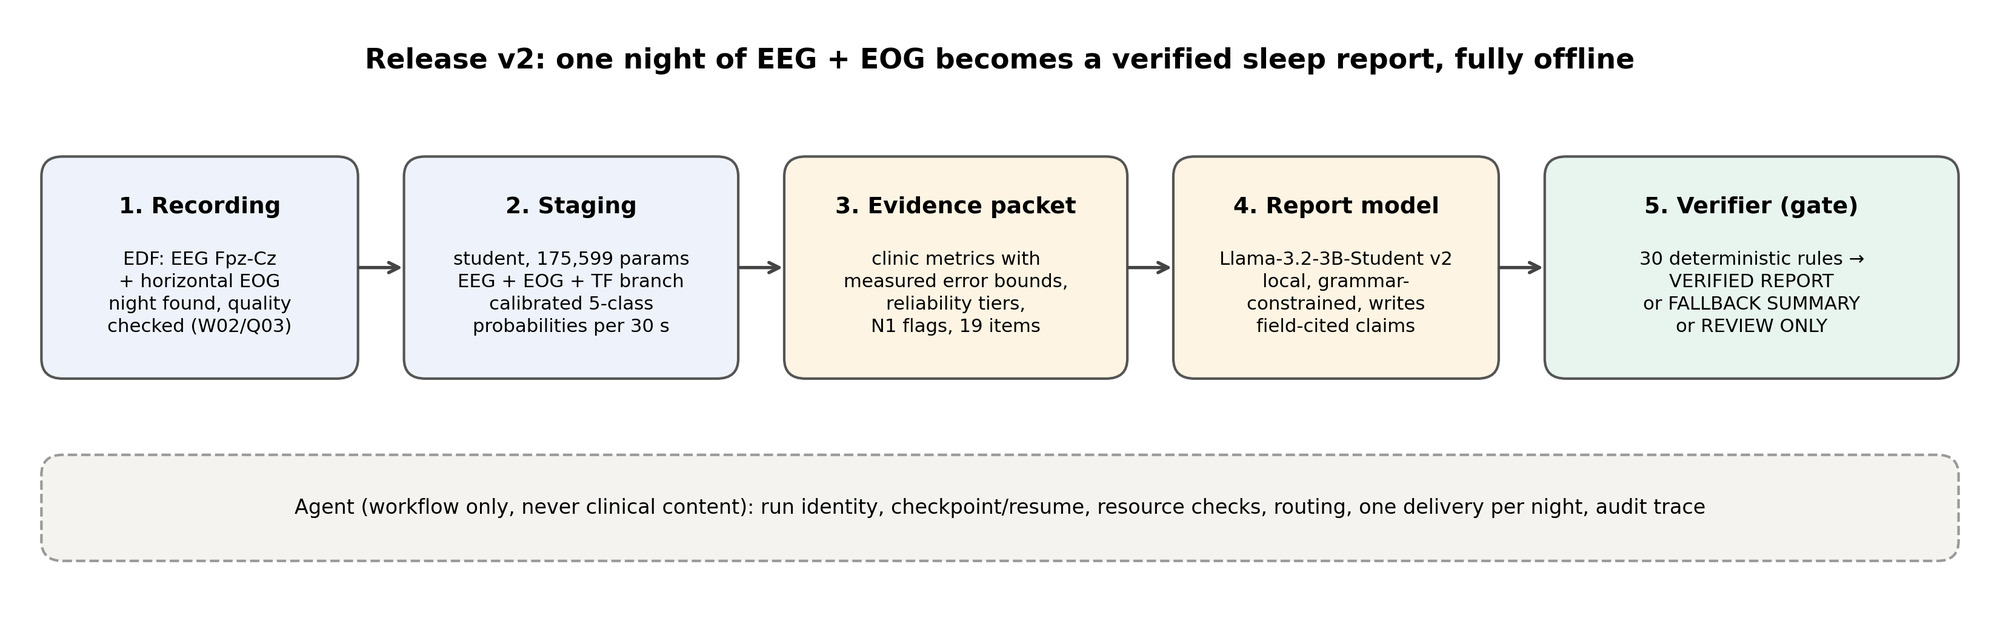
\includegraphics[width=\textwidth]{F33_system_overview.jpg}
\caption{System overview: one night of EEG + EOG becomes a verified sleep report, fully offline (release v2).}
\label{fig:overview}
\end{figure}

\subsection{ Objectives of the Proposed Work}

\begin{table}[htbp]
\centering\small
\caption{Measurable objectives.}
\label{tab:objectives}
\begin{tabularx}{\textwidth}{lYYl}
\toprule
\# & Objective & Measure & Target \\
\midrule
O1 & Leak-free staging evaluation & Subject-disjoint splits, checked in code & No subject in two splits \\
O2 & Compact, accurate student & Parameters; held-out $\kappa$ & $<$200\,K; $\ge$ teacher's $\kappa$ \\
O3 & Verified reports & Flawed reports released on the locked test set & 0 \\
O4 & Report completeness & Dev nights at 5/5 mandatory items & $\ge$25/31 (pre-registered) \\
O5 & Robust agent & Fault scenarios reaching the expected outcome & All \\
O6 & Edge readiness & Offline container: network off, no secrets, staging and report parity, ARM64 staging parity (emulated) & All met (container level) \\
\bottomrule
\end{tabularx}
\end{table}

\textbf{Secondary objectives:} calibrated confidence; measured reliability of each derived metric; byte-identical
reruns; graceful behaviour without the EOG channel; an edge budget within a Raspberry Pi 5's 16\,GB; a
plain-language summary for non-experts that only uses values the packet rates as reliable.

\section{ Methodology}

\subsection{Overview of the Approach:}

The work proceeded in six stages, each gated by a measured result before the next began (Figure~\ref{fig:pipeline}):

\begin{enumerate}
  \item \textbf{Knowledge distillation.} Audit the inherited model, rebuild subject-level splits, retrain the
  teacher, diagnose why naive KD failed, then fix the encoder and distil from an ensemble.
  \item \textbf{Student model.} Add an EOG branch, a time-frequency branch and local epoch context through gates
  that start closed; correct the labels; distil from the ensemble teacher (release v2).
  \item \textbf{Evidence packet.} Calibrate, decode the hypnogram, measure the error of every derived metric, fit
  the night-confidence tiers and the N1 flag on validation, and assemble the packet.
  \item \textbf{SLM.} Establish that the 30-rule contract is satisfiable with a large reference model, generate
  training targets, LoRA-tune small models, select on dev, evaluate once on test.
  \item \textbf{Agentic workflow.} Wrap the frozen pipeline in a deterministic state machine with quality checks,
  fallbacks and crash recovery; evaluate it with fault scenarios and invariants.
  \item \textbf{Edge simulation.} Budget time and memory analytically for a Raspberry Pi 5, then climb a simulation
  ladder (container limits, ARM64 emulation, fault replay, hardware) against pre-registered acceptance bars.
\end{enumerate}

\begin{figure}[htbp]
\centering
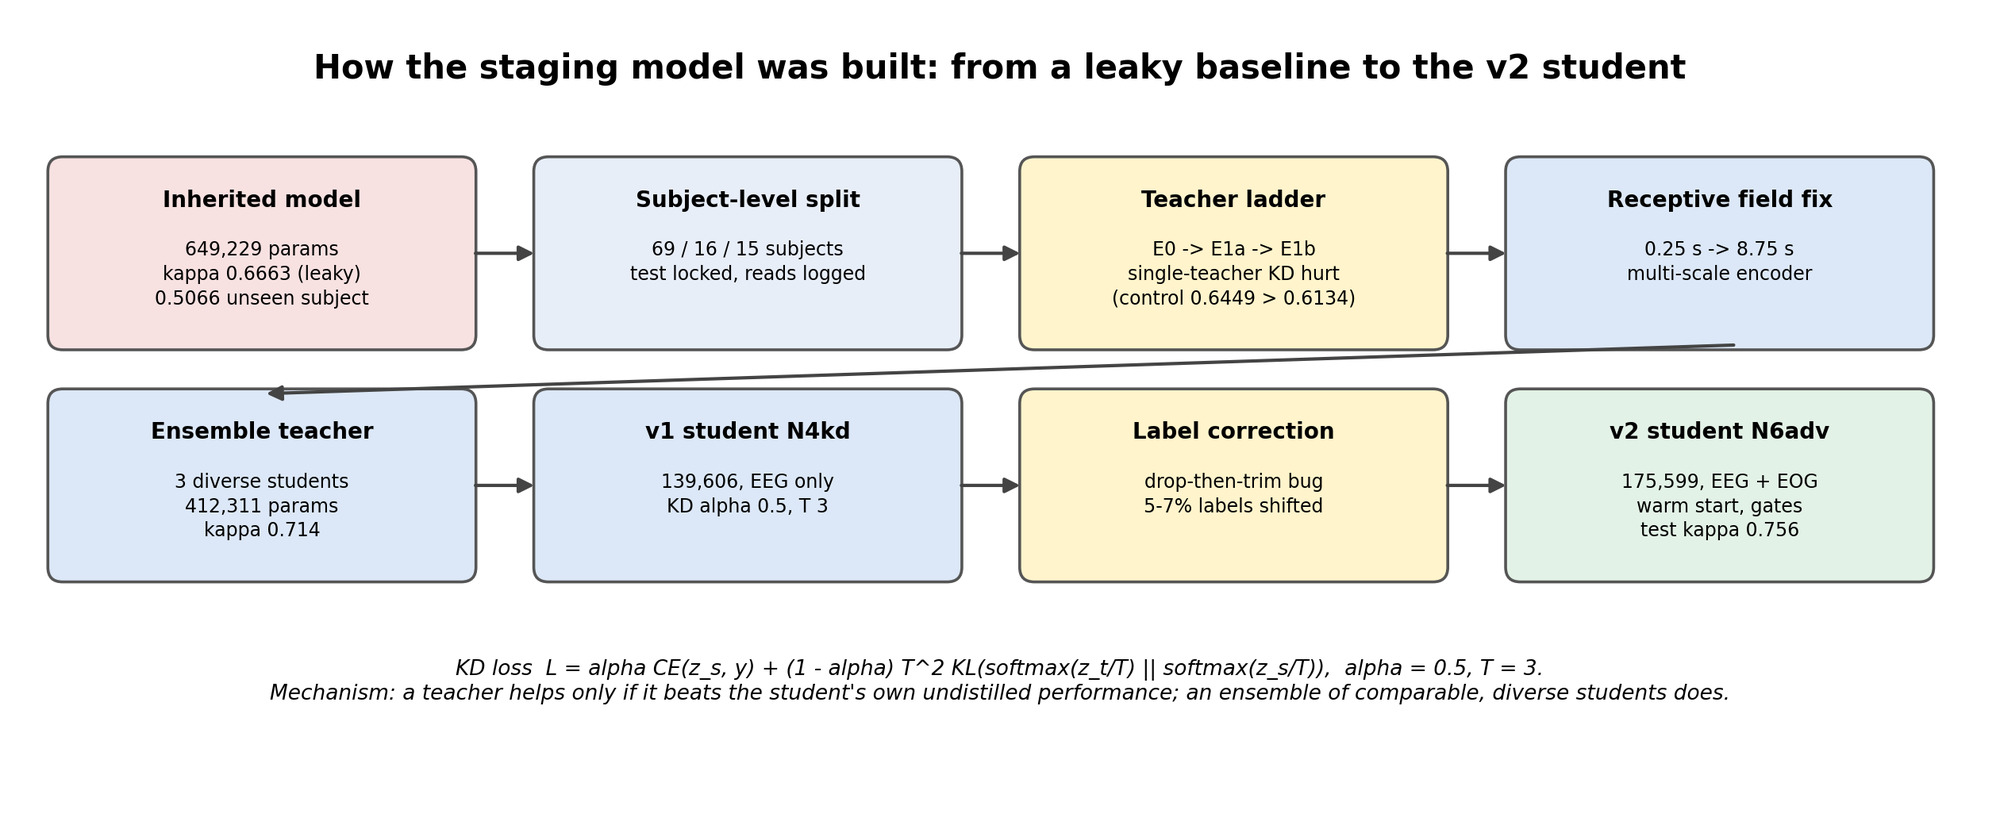
\includegraphics[width=\textwidth]{A5_training_pipeline.jpg}
\caption{How the staging model was built, from the leaky inherited baseline to the v2 student.}
\label{fig:pipeline}
\end{figure}

\subsection{Dataset Selection:}\label{sec:dataset}

\textbf{Sleep-EDFx} (PhysioNet)~\cite{kemp2000sleepedf,goldberger2000physionet}: 197 recordings (153 SC + 44 ST)
from 100 subjects; 237,950 scored epochs. Each epoch has 3,000 EEG samples (Fpz-Cz, 100\,Hz) and 34 spectral
features: for each of the six db4 wavelet sub-bands (5 levels) its energy, log-energy, entropy and variance (24), plus
STFT relative band powers (delta, theta, alpha, beta, gamma), spectral entropy, 95\% spectral edge frequency and three
band ratios (10). Release v2 adds the horizontal EOG and 8 EOG features per epoch: four band log-powers (0.3--8\,Hz),
log-variance, saccade rate, mean absolute derivative and the EOG--EEG correlation. Class shares: N2 37.4\%, W 29.5\%, REM 14.4\%, N1 10.6\%, N3 8.2\%.

Almost every subject was recorded on two consecutive nights, so a recording-level split puts the same person in
training and test. All splits are made \textbf{by subject} (first five characters of the recording ID), stratified
by cohort, and checked in code (Table~\ref{tab:splits}, Figure~\ref{fig:split}).

\begin{table}[htbp]
\centering\small
\caption{Dataset and split summary.}
\label{tab:splits}
\begin{tabularx}{\textwidth}{lrrrrY}
\toprule
Split & Subjects & Recordings & SC subj. & ST subj. & Role \\
\midrule
Train & 69 & 137 & 54 & 15 & Staging and SLM training (123 + 14 nights for the SLM) \\
Validation (dev) & 16 & 31 & 12 & 4 & Calibration, tier fitting, model selection \\
\textbf{Test (locked)} & \textbf{15} & \textbf{29} & 12 & 3 & One logged evaluation per model \\
5-fold CV & 85 & 168 & -- & -- & Architecture ablation (non-test subjects) \\
B1 benchmark & 78 & 153 & 78 & -- & Standard 10-fold subject-wise protocol \\
\bottomrule
\end{tabularx}
\end{table}

\begin{figure}[htbp]
\centering
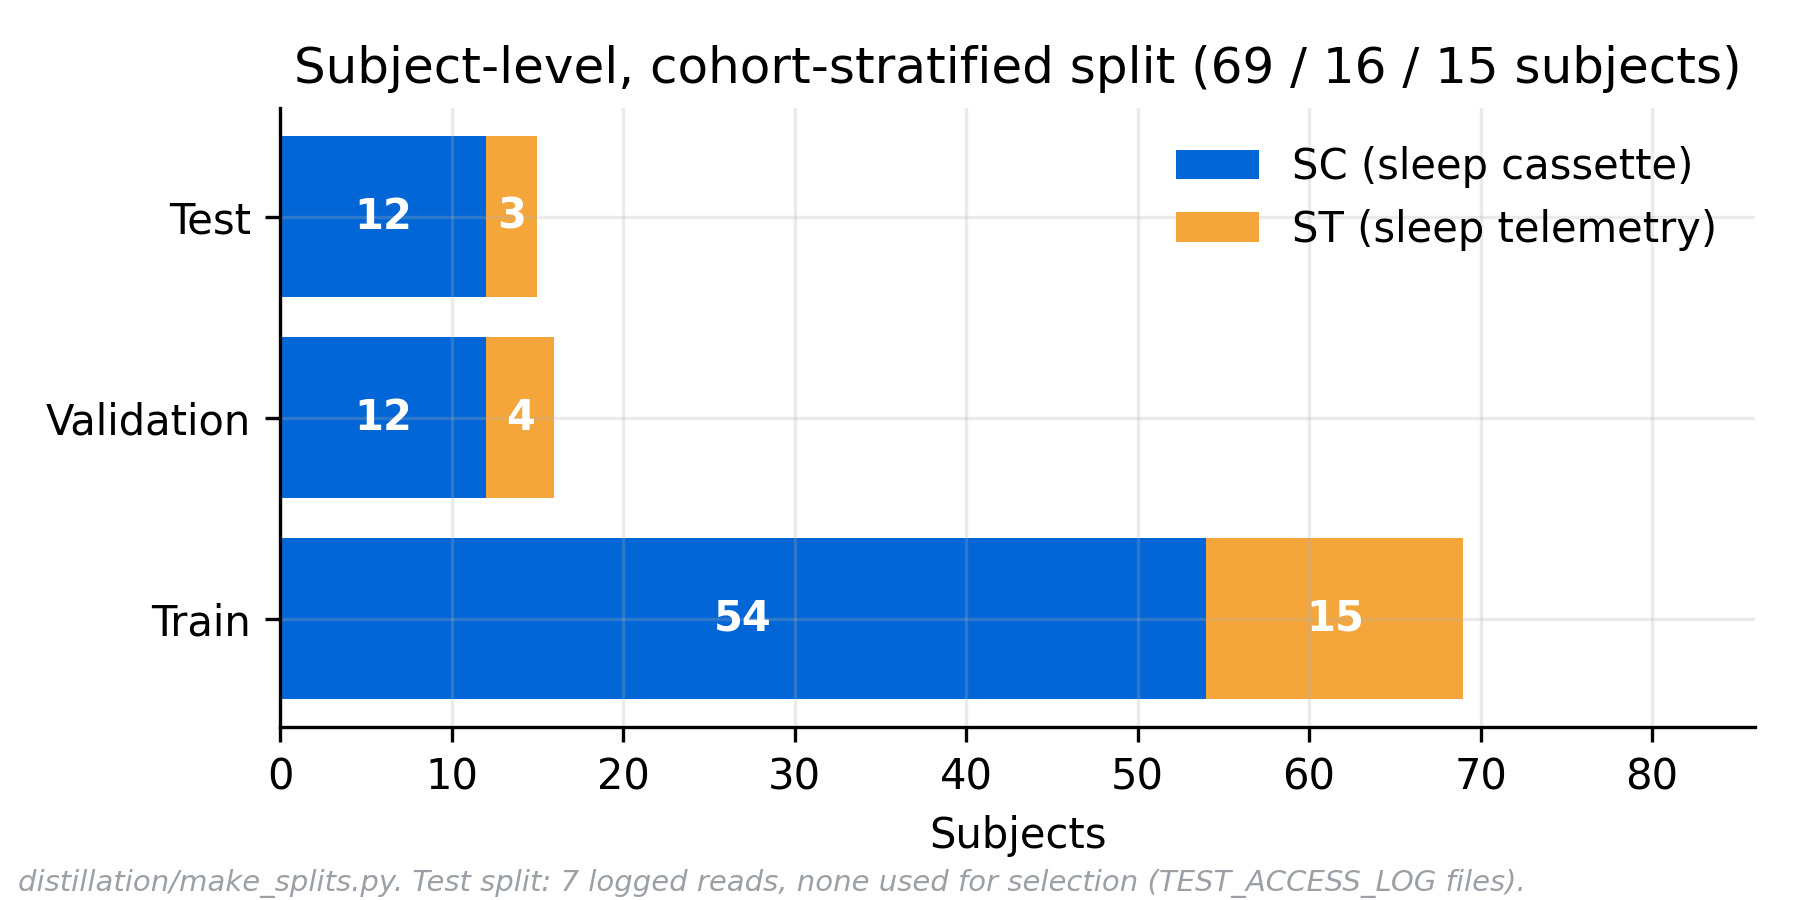
\includegraphics[width=0.85\textwidth]{F1_subject_split.jpg}
\caption{Subject-level split. Every read of the test labels is logged; none was used for selection.}
\label{fig:split}
\end{figure}

\textbf{Label correction.} The original preprocessing removed unscored epochs from the label sequence \emph{before}
computing trim points, then cut the full signal with those points, so each dropped epoch shifted every later label
by one epoch. Rebuilt from the raw hypnograms, the corrected labels change 5.65\% of training labels, 7.10\% of
validation and 5.17\% of test. \textbf{All release v2 numbers use corrected labels.} v1-era numbers in
Section~\ref{sec:res-kd} use the original \emph{stored} labels and are not comparable with v2's.

\textbf{Plain-language reference data.} For the non-expert summary, age-specific reference ranges were taken from
the National Sleep Foundation consensus~\cite{ohayon2017nsf}, Watson et al.~\cite{watson2015} and Ohayon et
al.~\cite{ohayon2004meta}, together with each subject's age, sex and cohort from the Sleep-EDF metadata.

\subsection{Algorithm/Model Design:}

\textbf{System architecture.} Figure~\ref{fig:arch} shows the three layers of the system. \emph{Offline}, run once on
a Kaggle T4 GPU, the data are split and corrected, the staging model is distilled, the packet tables are fitted on
validation and the report model is fine-tuned. Their products become the \emph{release}: a YAML file
(\texttt{agentic/config/releases/v2.yaml}) that names every file the system runs and pins it by sha256 (execution
manifest \texttt{4973f498\ldots}). At \emph{runtime}, on the device, the agent walks a raw EDF through ingest and
quality control, preprocessing, two-pass staging, packet building, report generation, the verifier and delivery,
loading each pinned file at the step that uses it. Swapping a model means writing a new release file, not new agent
code.

\begin{figure}[htbp]
\centering
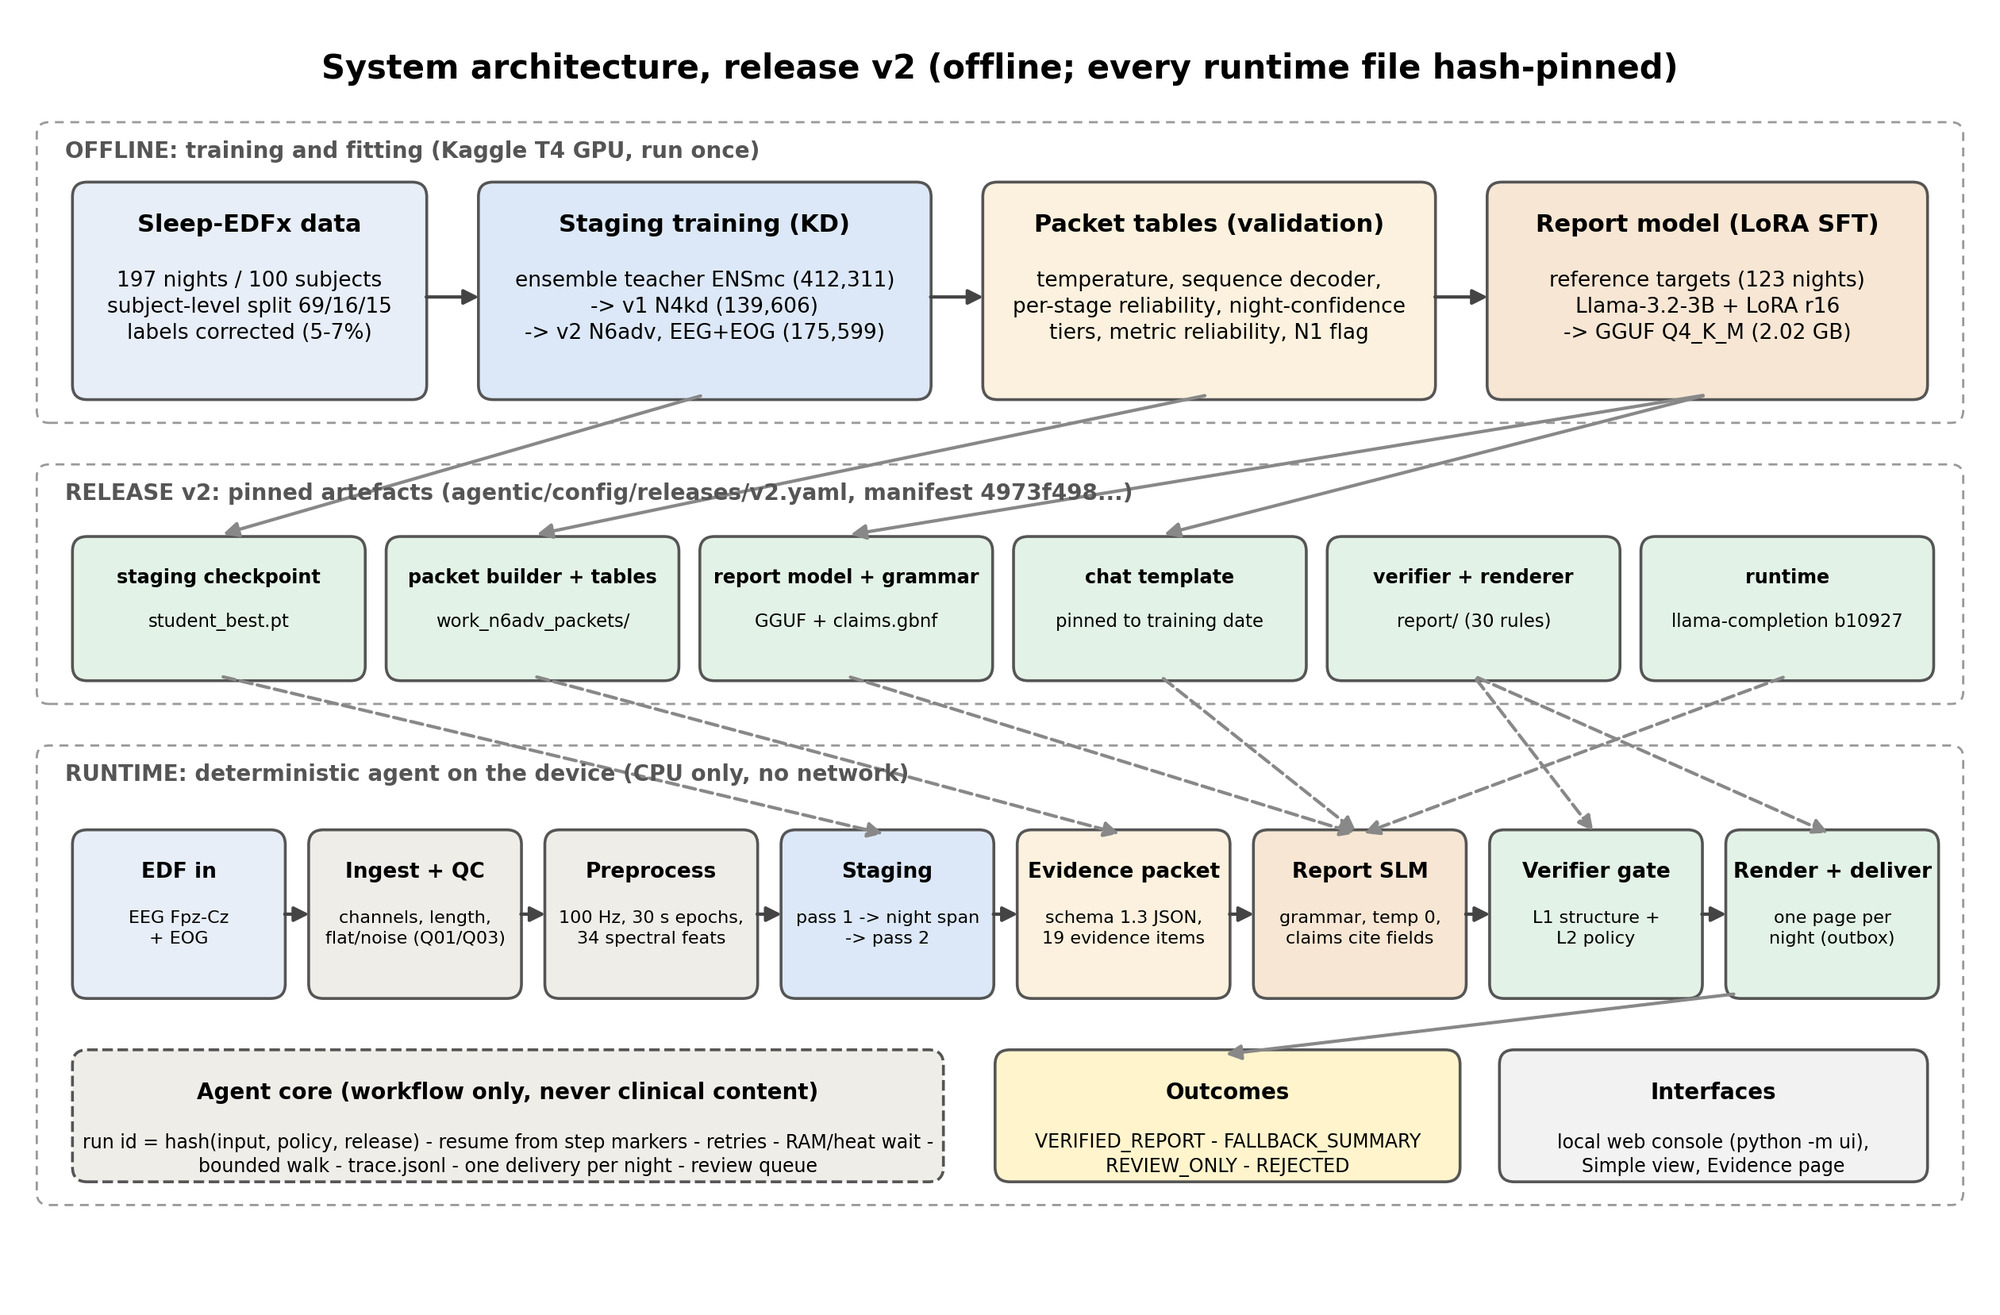
\includegraphics[width=\textwidth]{A1_system_architecture.jpg}
\caption{System architecture of release v2: offline training, the hash-pinned release, and the runtime agent pipeline.}
\label{fig:arch}
\end{figure}

\textbf{Block-wise view.} Figure~\ref{fig:blockwise} opens the same system block by block, from the input tensors to
the delivered page: (1) inputs and the 34 + 8 per-epoch features; (2) the gated multi-branch encoder with its
parameter budget against the teacher's; (3) the Transformer sequence model; (4) the distillation objective and its
result; (5) the evidence packet, the only thing downstream modules may read; (6) the report model and the two-layer
verifier; (7) the agent, delivery and the edge target. Each block also carries its measured headline result.

\begin{figure}[p]
\centering
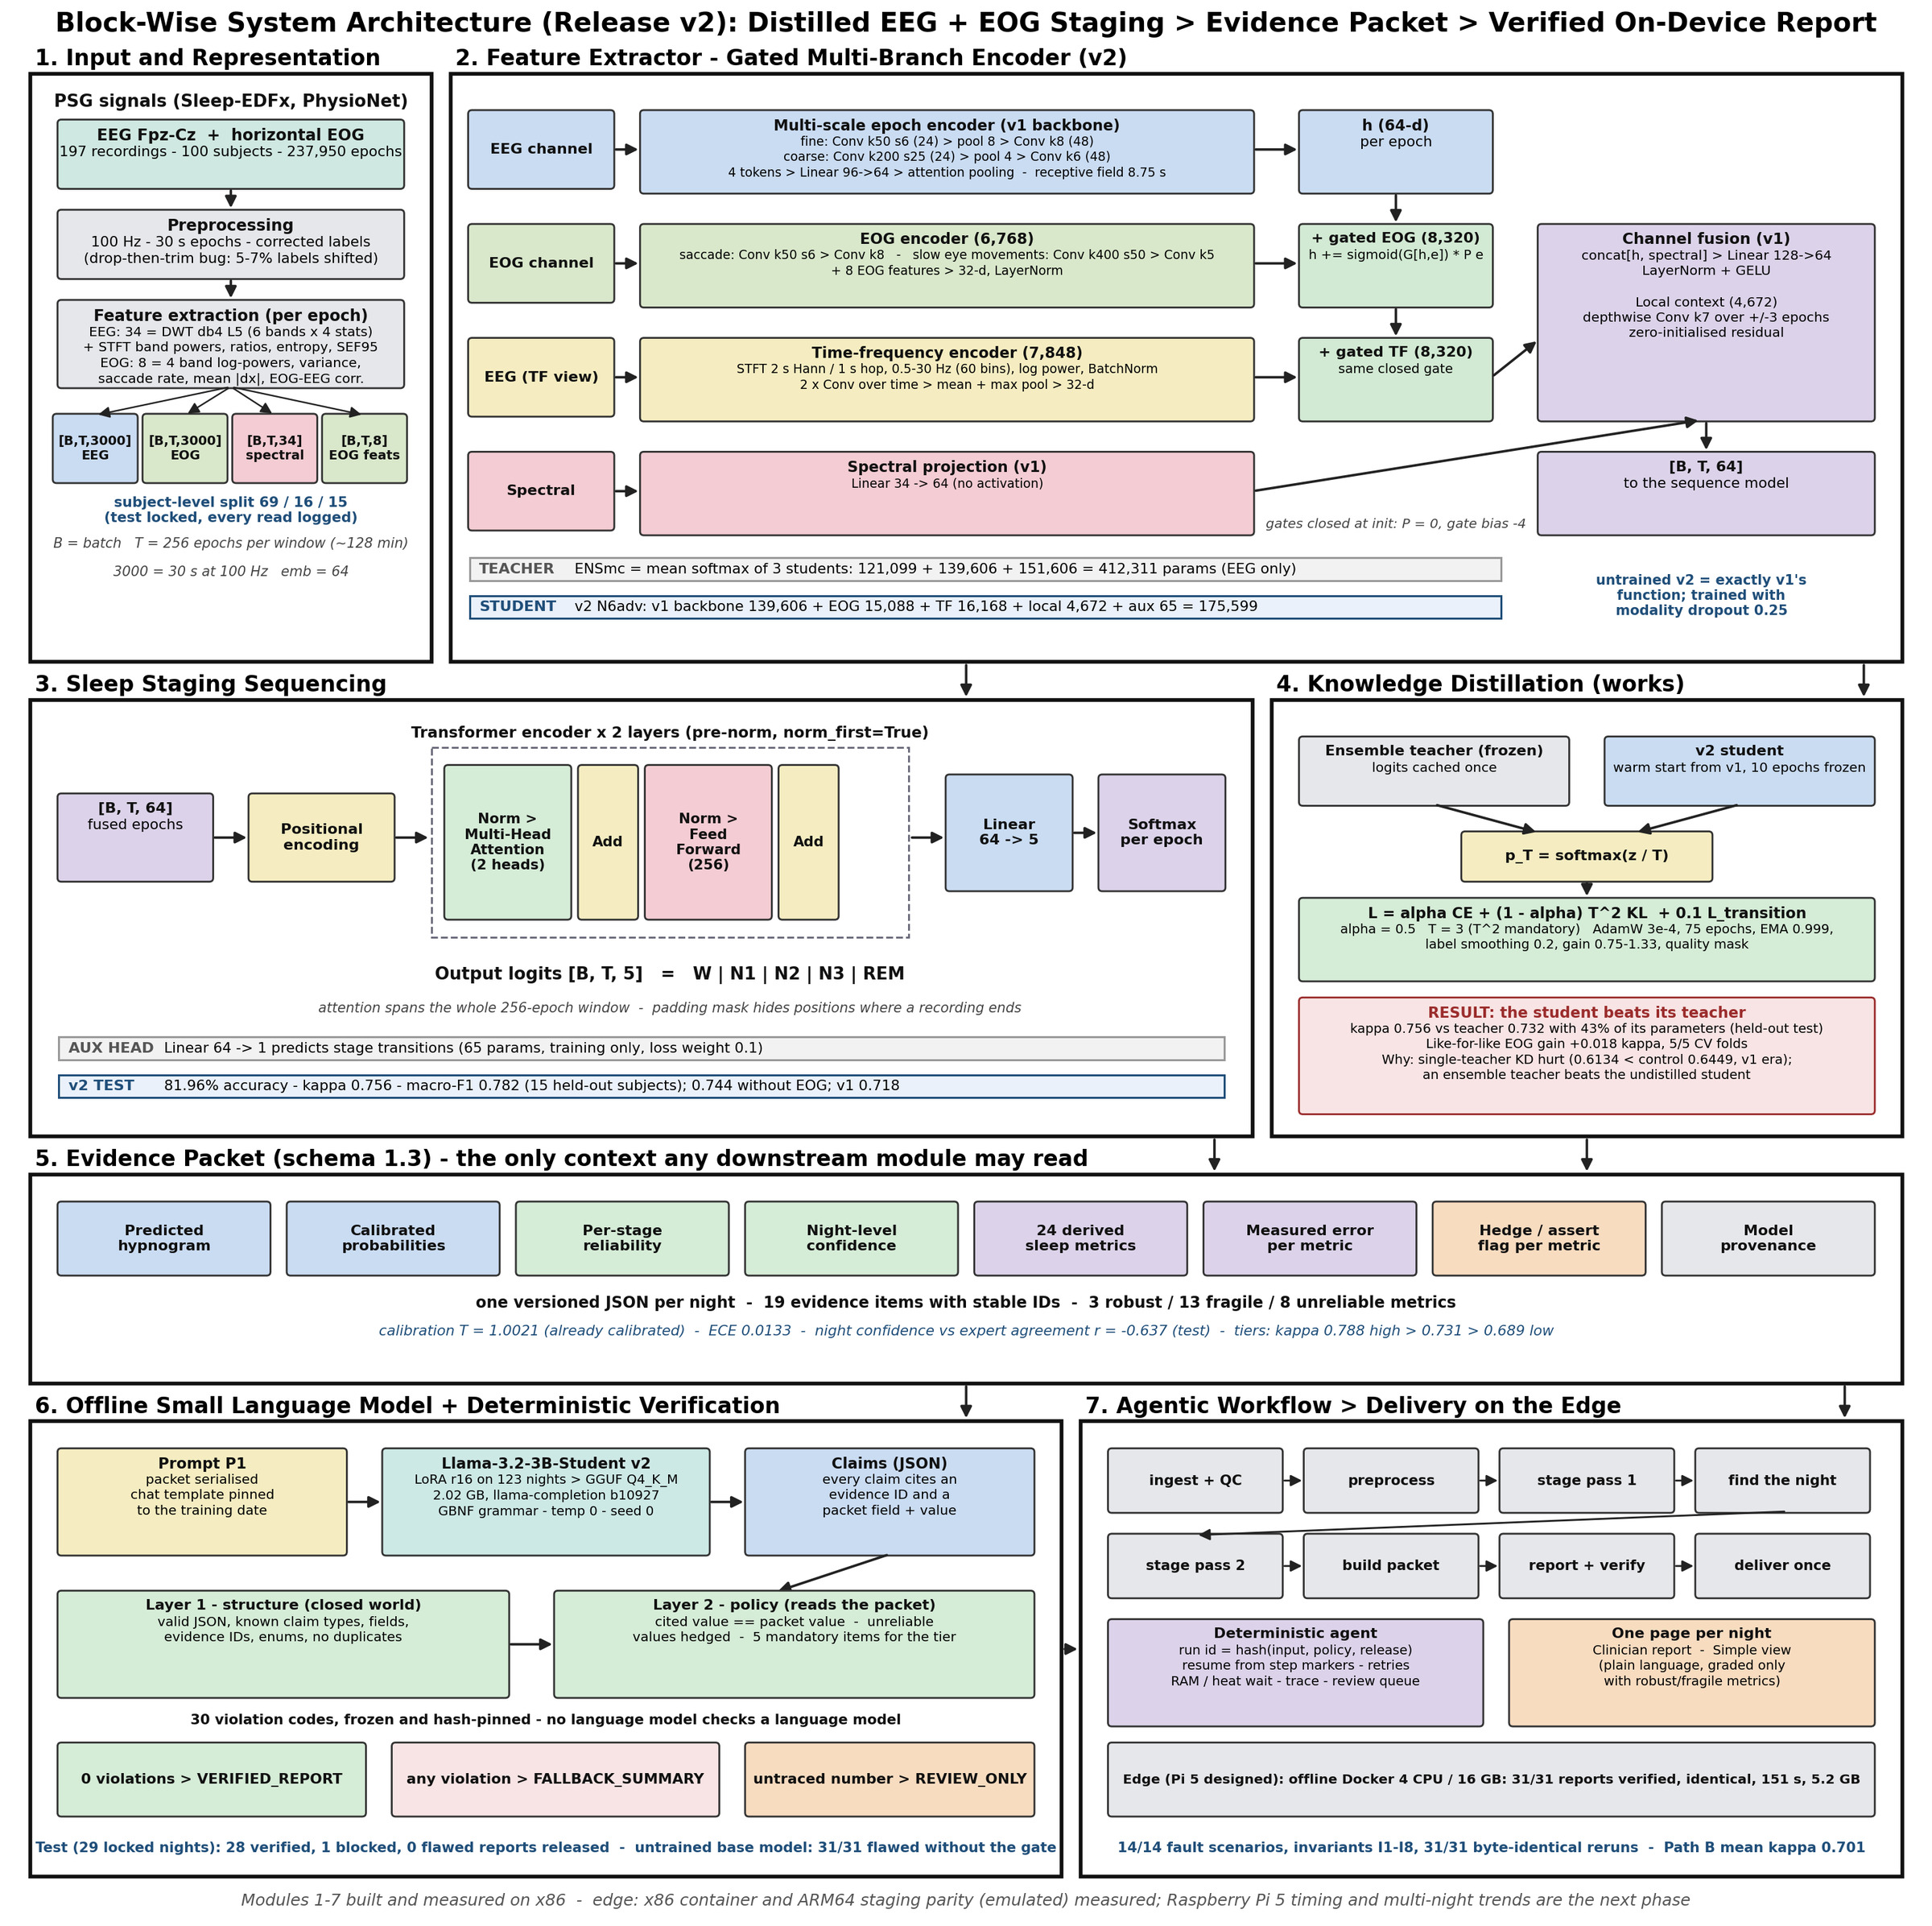
\includegraphics[width=\textwidth]{A0_blockwise_architecture_v2.jpg}
\caption{Block-wise architecture of release v2, with each block's measured result.}
\label{fig:blockwise}
\end{figure}

\textbf{Teacher.} The ensemble teacher ENSmc averages the softmax of three students of the same family
(121,099 + 139,606 + 151,606 = \textbf{412,311} parameters). It replaced a single 649,229-parameter teacher after
the experiments in Section~\ref{sec:res-kd}.

\textbf{Student, release v1 (N4kd, 139,606 parameters, historical).} One EEG channel plus 34 spectral features, read
as sequences of 256 epochs (about 2\,h). A multi-scale epoch encoder has a fine branch (Conv k50 s6, 24 channels
$\rightarrow$ max-pool 8 $\rightarrow$ Conv k8, 48) and a coarse branch (Conv k200 s25, 24 $\rightarrow$ max-pool 4
$\rightarrow$ Conv k6, 48); both are pooled to 4 tokens, projected 96$\rightarrow$64 and attention-pooled into a
64-d epoch vector. The spectral features are projected 34$\rightarrow$64, fused (Linear, LayerNorm, GELU), given
sinusoidal positions and passed through a 2-layer pre-norm Transformer encoder (d 64, 2 heads, FF 256) with a
5-class head. The encoder's measured receptive field is \textbf{8.75\,s}, wide enough to contain a spindle,
K-complex or slow wave; the original encoder's was 25 samples (0.25\,s) (Figure~\ref{fig:rf}).

\begin{figure}[htbp]
\centering
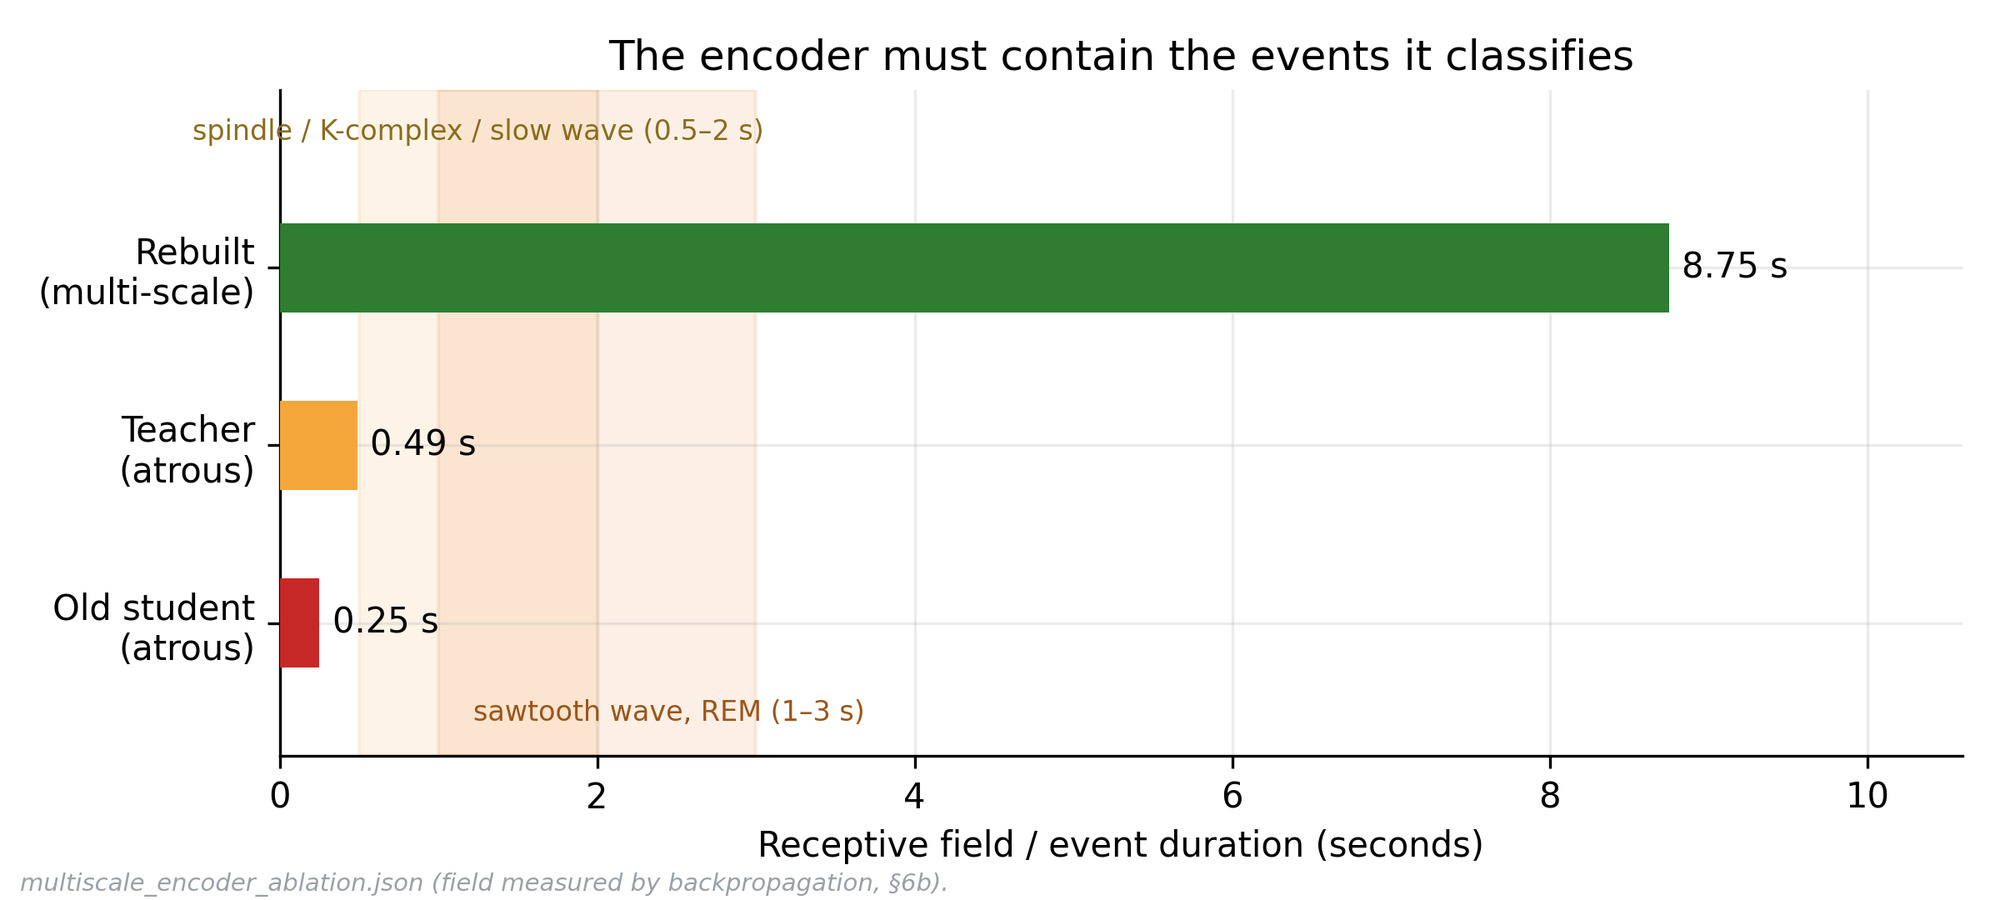
\includegraphics[width=0.8\textwidth]{v1_F5_receptive_field.jpg}
\caption{Measured receptive field of the original (0.25\,s) and multi-scale (8.75\,s) encoders.}
\label{fig:rf}
\end{figure}

\textbf{Student, release v2 (N6adv ``full'', 175,599 parameters, current).} The v1 backbone is kept unchanged and
three parts are added, each joining through a \textbf{gate that starts closed}: the projection is zero-initialised
and the gate bias is $-4$, so at initialisation the model computes exactly v1's function and moves away only where
that helps (Figure~\ref{fig:student}, Table~\ref{tab:params}). For an epoch representation $h$ and a branch output
$e$, each gated branch adds
\begin{equation}
h \leftarrow h + \sigma\!\left(W_g [h; e] + b_g\right) \odot P e, \qquad P = 0,\; b_g = -4 \text{ at initialisation.}
\end{equation}
The gated EOG and time-frequency residuals are added to $h$ in turn, then $h$ is fused with the spectral
projection, refined by a zero-initialised local-context convolution over $\pm3$ neighbouring epochs, and passed to
the Transformer.

\begin{figure}[htbp]
\centering
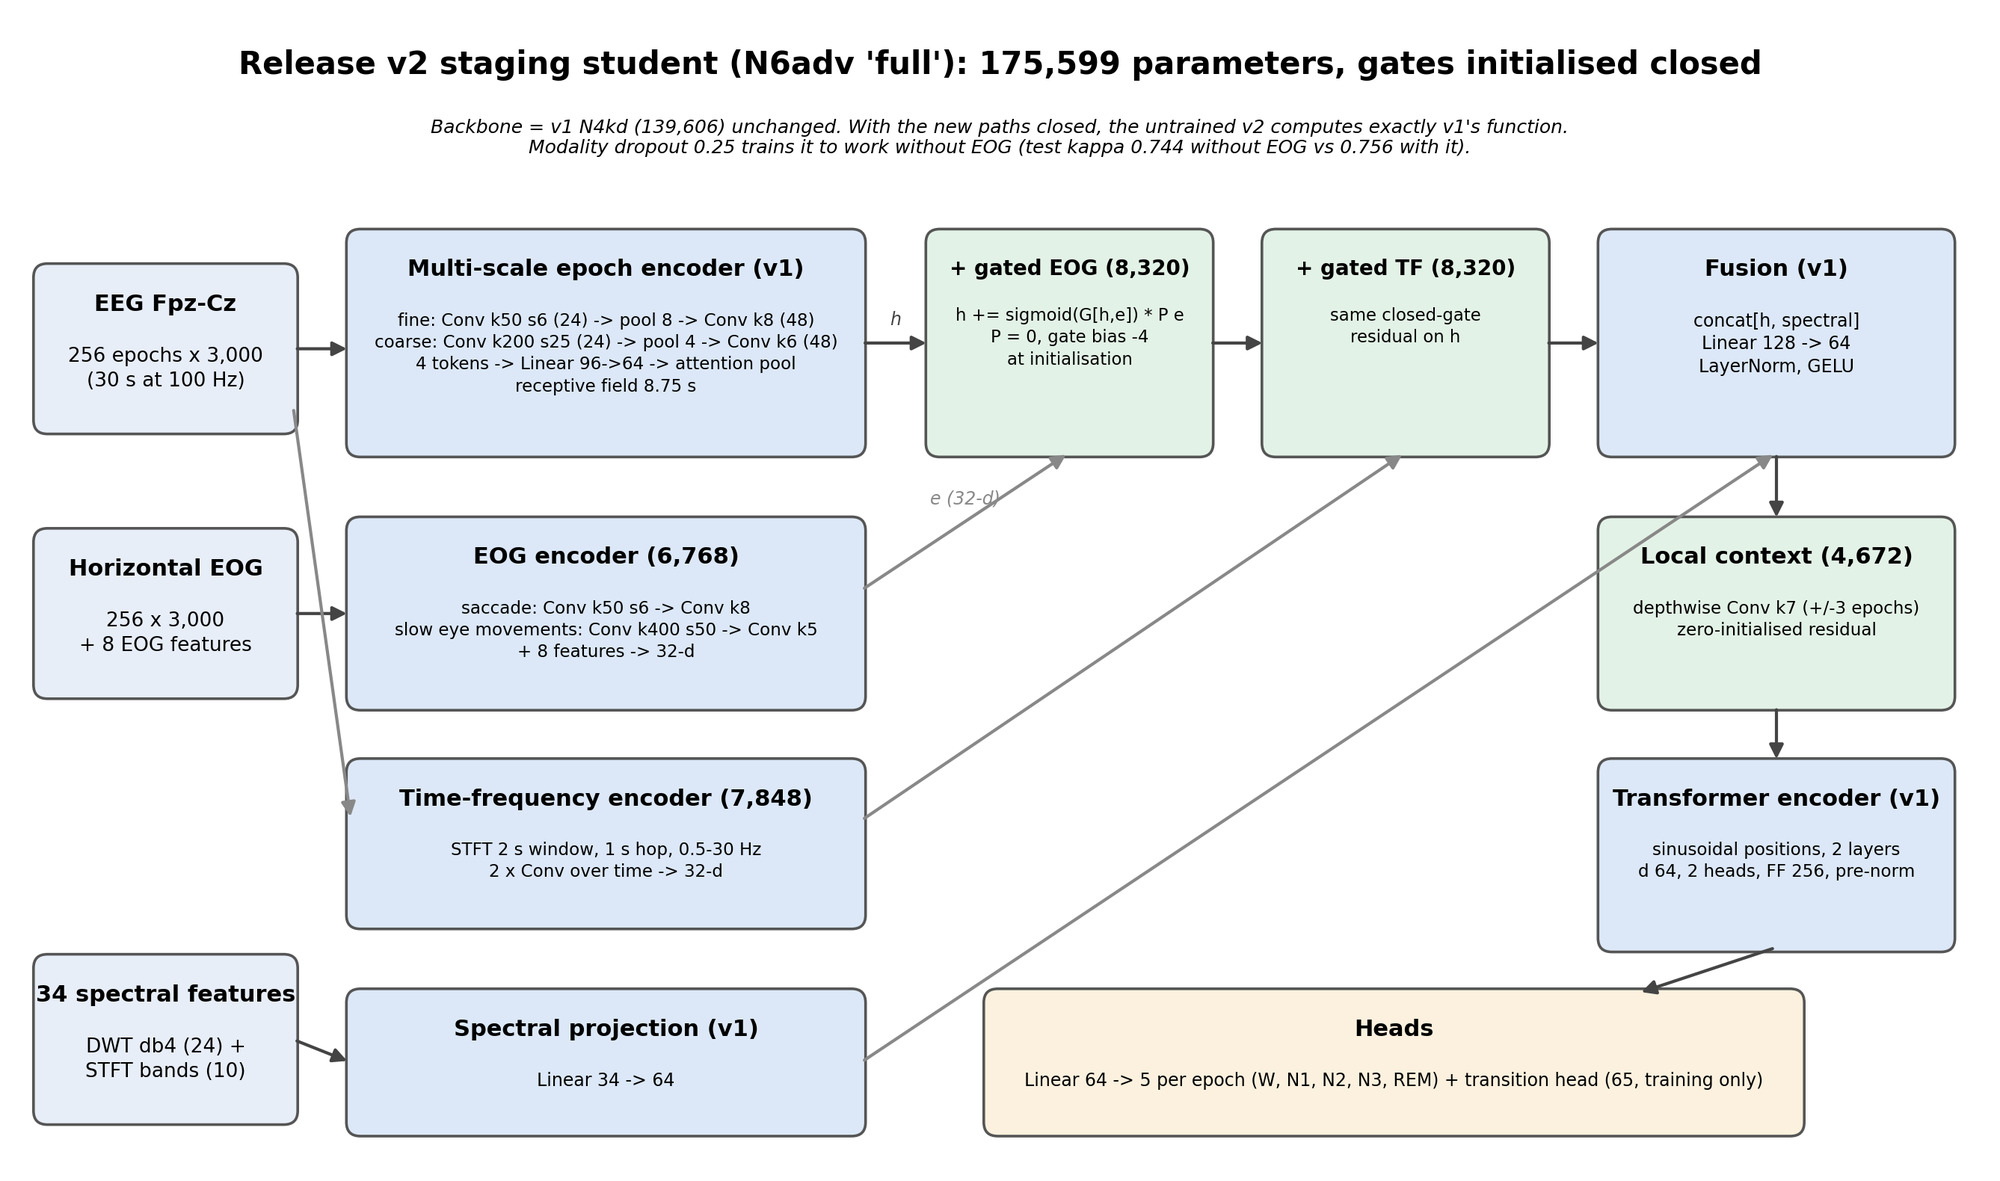
\includegraphics[width=\textwidth]{A2_staging_model_v2.jpg}
\caption{Architecture of the release v2 staging student (from \texttt{AdvancedStudent} in the training code).}
\label{fig:student}
\end{figure}

\begin{table}[htbp]
\centering\small
\caption{Release v2 staging student: parameter budget.}
\label{tab:params}
\begin{tabularx}{\textwidth}{lYr}
\toprule
Part & What it does & Params \\
\midrule
v1 backbone & Multi-scale encoder, spectral projection, fusion, Transformer, head (unchanged) & 139,606 \\
EOG encoder & Saccade branch (Conv k50 s6) + slow-eye-movement branch (Conv k400 s50) + 8 hand-made EOG features $\rightarrow$ 32-d & 6,768 \\
EOG projection + gate & 32 $\rightarrow$ 64, sigmoid gate on $[h, e]$ & 8,320 \\
Time-frequency encoder & STFT (2\,s window, 1\,s hop), 0.5--30\,Hz in 0.5\,Hz bins, 2 convolutions $\rightarrow$ 32-d & 7,848 \\
TF projection + gate & 32 $\rightarrow$ 64, sigmoid gate & 8,320 \\
Local context & Depthwise conv k7 over $\pm$3 epochs, zero-initialised & 4,672 \\
Auxiliary transition head & Predicts stage changes (training only) & 65 \\
\midrule
\textbf{Total} & & \textbf{175,599} \\
\bottomrule
\end{tabularx}
\end{table}

\textbf{Evidence packet.} A deterministic builder turns per-epoch probabilities into a versioned JSON packet
(Table~\ref{tab:packet}). Fields that are not yet populated are present and \texttt{null}, so adding them later
does not break consumers.

\begin{table}[htbp]
\centering\small
\caption{Evidence packet schema 1.3 (top-level fields).}
\label{tab:packet}
\begin{tabularx}{\textwidth}{lY}
\toprule
Field & Content \\
\midrule
\texttt{schema\_version} & "1.3"; consumers refuse a mismatch \\
\texttt{recording\_id}, \texttt{subject\_id}, \texttt{cohort} & Identity \\
\texttt{provenance} & Model, checkpoint sha256, git commit, calibration temperature, decoder, generator \\
\texttt{hypnogram}, \texttt{decoding} & Predicted stages, stage runs, how the hypnogram was decoded \\
\texttt{probabilities} & Calibrated per-epoch probabilities, 5 classes \\
\texttt{per\_stage} & Counts, mean confidence, model reliability tier per stage \\
\texttt{derived\_metrics} & 24 metrics (TST, efficiency, WASO, REM latency, \ldots) \\
\texttt{derived\_metric\_reliability} & Which metrics may be asserted: robust / fragile / unreliable, from measured error \\
\texttt{night\_confidence} & Tier and mean entropy; no ground truth needed \\
\texttt{evidence\_items} & 19 items with stable IDs that claims must cite \\
\texttt{attribution}, \texttt{risk} & Integrated-Gradients profile (v1 packets); risk reserved \\
\bottomrule
\end{tabularx}
\end{table}

\textbf{Report model and verifier (Figure~\ref{fig:verifier}).} Llama-3.2-3B-Instruct~\cite{llama32} with LoRA
adapters~\cite{hu2022lora}, quantised to Q4\_K\_M (2.02\,GB), is run by \texttt{llama-completion} (llama.cpp
b10927~\cite{llamacpp}) under a GBNF grammar that admits only the claim schema, at temperature 0 and seed 0, with a
chat template pinned to its training date. The verifier has two layers. Layer~1 (structure, packet-independent)
owns the closed world: valid JSON, known claim types, fields, evidence IDs and enums, no duplicates. Layer~2
(policy, reads the packet) checks that every cited value equals the packet's value exactly, that unreliable values
are hedged, that nothing is double-counted, that no unsafe item is cited without a review flag, and that the five
mandatory items for the night's tier are covered --- 30 violation codes in total. A rendered page passes a final
V-HTML check that every number on it traces to the packet.

\begin{figure}[htbp]
\centering
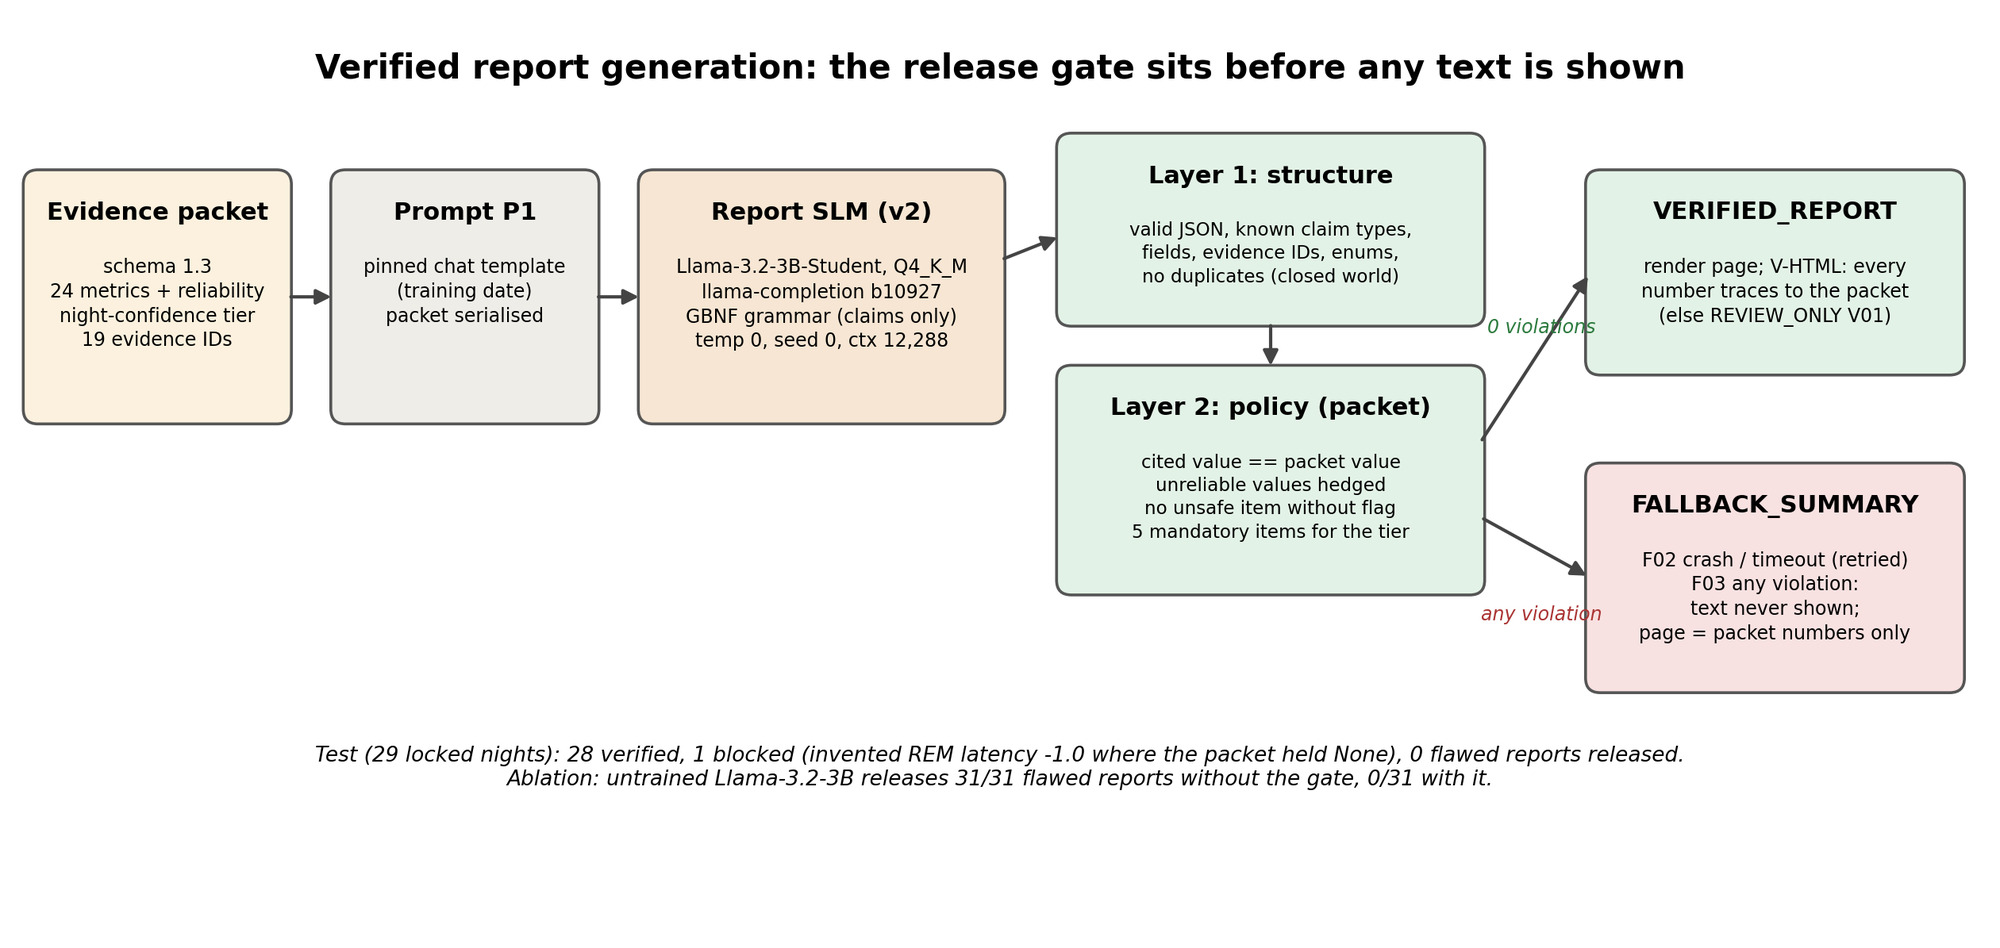
\includegraphics[width=\textwidth]{A3_report_and_verifier.jpg}
\caption{Verified report generation: the release gate sits before any text is shown.}
\label{fig:verifier}
\end{figure}

\textbf{Agent (Figure~\ref{fig:agent}).} A state machine whose steps each write to their own directory and return a
decision naming the next step. Run identity is a hash of the input, the policy and the release manifest. Finished
steps are replayed from their markers, an interrupted step is wiped and re-run, every transition is traced, and the
walk is bounded so a run always ends. Path~A starts from a prebuilt packet; Path~B starts from a raw EDF with no
expert hypnogram.

\begin{figure}[htbp]
\centering
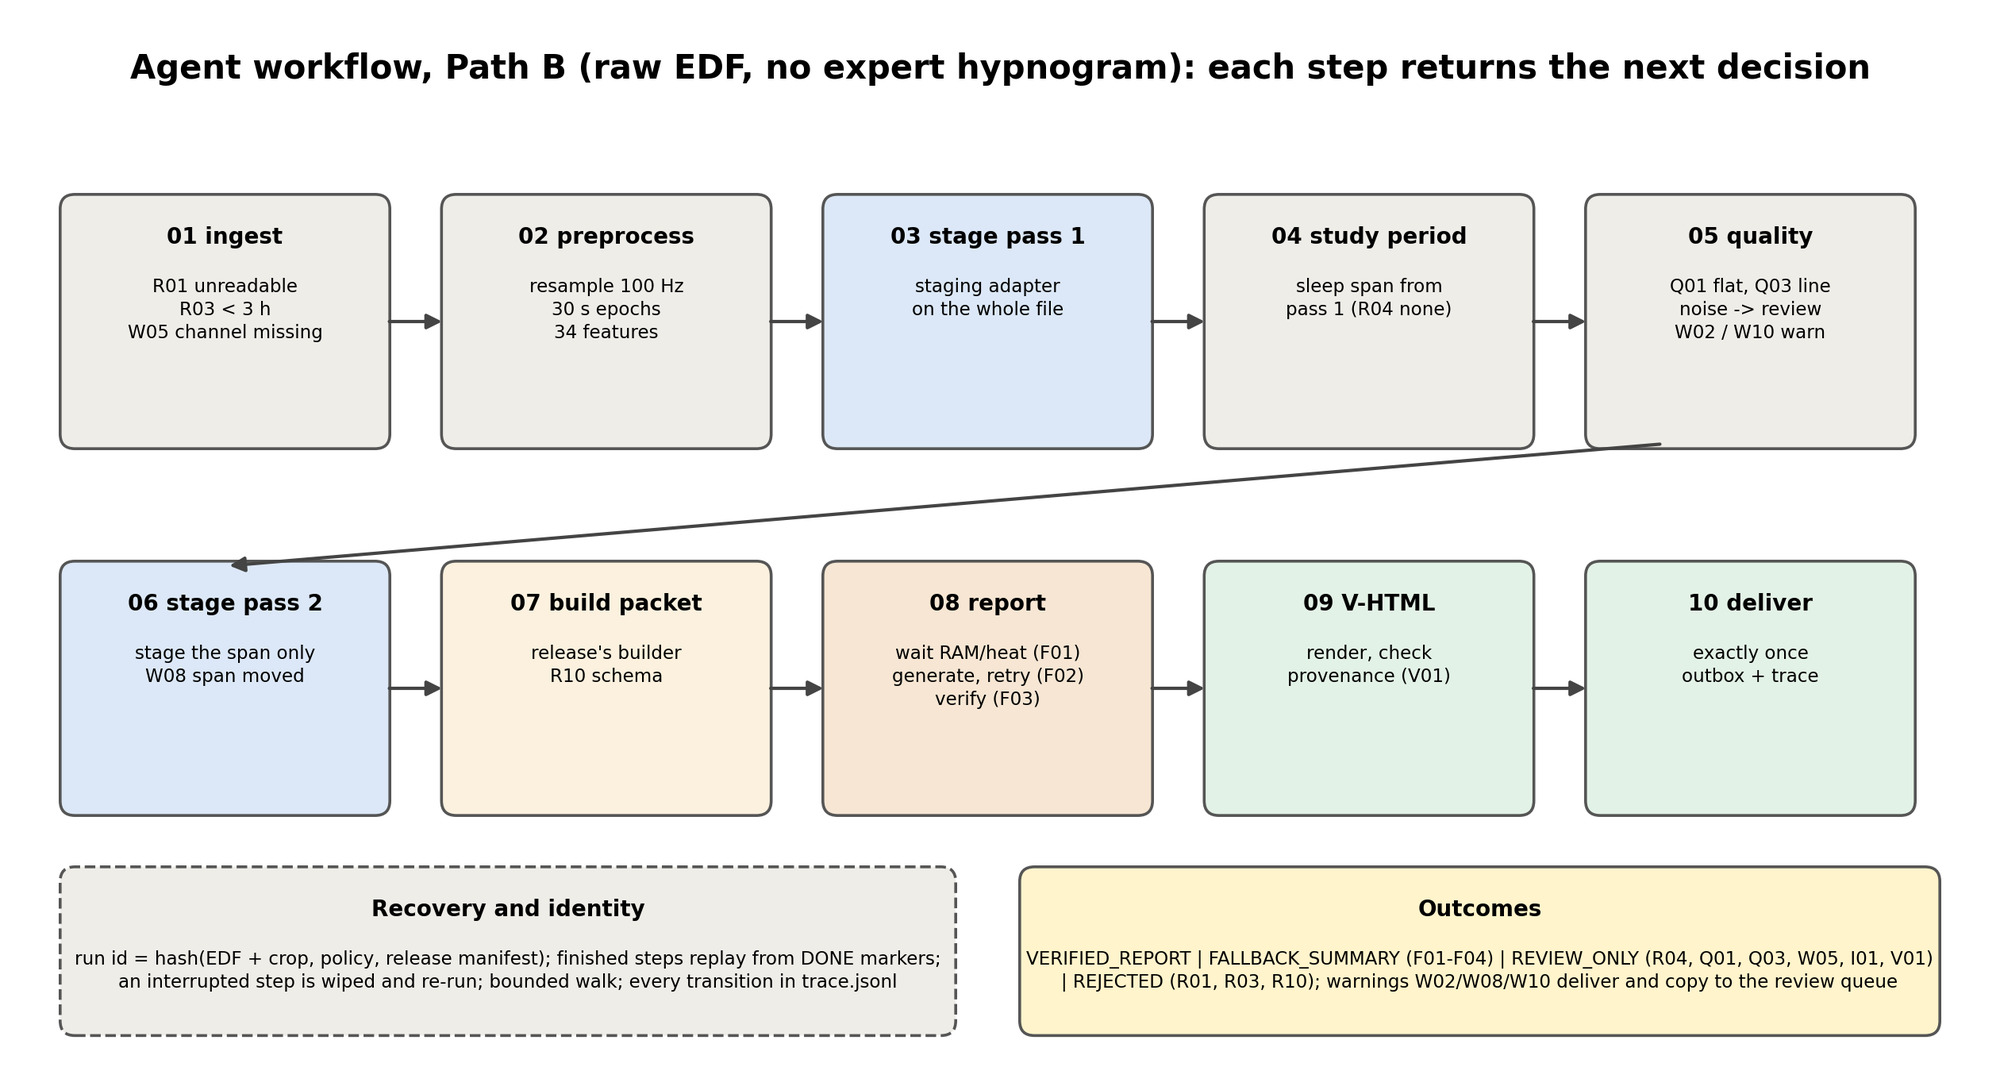
\includegraphics[width=\textwidth]{A4_agent_workflow.jpg}
\caption{Agent workflow, Path B: each step returns the next decision; reason codes name every exit.}
\label{fig:agent}
\end{figure}

\textbf{Plain-language layer.} A deterministic, template-based summary for non-experts grades the packet's values
against age-specific reference ranges. It shows only robust and fragile metrics in the main text (fragile ones
with "could be off by about X"), moves unreliable ones to "details for your doctor", always states what the test
cannot detect, and is checked by a self-test that every number traces to the packet or the reference table. It is
not written by the language model.

\subsection{Tools and Technologies:}

\begin{table}[htbp]
\centering\small
\caption{Tools and technologies.}
\label{tab:tools}
\begin{tabularx}{\textwidth}{lY}
\toprule
Area & Tools \\
\midrule
Language & Python 3 \\
Signal processing & MNE (EDF reading, resampling), PyWavelets (DWT), SciPy (STFT, Welch for EOG), NumPy, pandas \\
Staging models & PyTorch; trained on Kaggle (NVIDIA T4) \\
Report model & Hugging Face Transformers + PEFT (LoRA) on Kaggle T4; llama.cpp b10927 for GGUF Q4\_K\_M inference on CPU \\
Reference model & Gemini 3.1 Flash, used once offline to establish the contract and generate training targets \\
Constrained decoding & GBNF grammar \\
Agent & Plain-Python state machine, YAML release manifests and policy, sha256 pinning, atomic file writes \\
Interface & FastAPI + Uvicorn local console (\texttt{python -m ui}), static HTML/JS, no external assets \\
Testing & pytest (agent, KD loss, splits, provenance), fault injection \\
Edge & Docker (CPU and memory limits, \texttt{--network none}), QEMU/buildx for ARM64; Raspberry Pi 5 (designed) \\
\bottomrule
\end{tabularx}
\end{table}

\subsection{Algorithm or Model Description}

\textbf{Knowledge-distillation loss.} For student logits $z_s$, teacher logits $z_t$, labels $y$, mixing weight
$\alpha$ and temperature $T$:
\begin{equation}
\mathcal{L} = \alpha\,\mathrm{CE}(z_s, y) + (1-\alpha)\,T^2\,\mathrm{KL}\!\left(\mathrm{softmax}(z_t/T)\,\Vert\,\mathrm{softmax}(z_s/T)\right),
\end{equation}
with $\alpha = 0.5$ and $T = 3$. The $T^2$ factor keeps the soft-target gradient on the same scale as the hard-label
gradient; without it training still runs but silently learns worse, so a unit test covers it. Teacher outputs are
cached once rather than recomputed every epoch.

\begin{algorithm}[htbp]
\caption{Ensemble-teacher distillation of the staging student}\label{alg:kd}
\begin{algorithmic}[1]
\State \textbf{Input} subject-disjoint training recordings $R$; trained students $S_1 \ldots S_K$; architecture $A$; $\alpha$, $T$
\State \textbf{Output} distilled student $S^*$
\For{each recording $r \in R$}
  \State $z_t[r] \gets \log\!\big(\tfrac{1}{K}\sum_k \mathrm{softmax}(S_k(r))\big)$ \Comment{ensemble teacher, cached}
\EndFor
\State initialise $S^*$ from $A$ (warm start from the v1 backbone; new gates closed)
\For{epoch $= 1 \ldots 75$}
  \For{each batch of 256-epoch sequences $(x, y, r)$}
    \State $\mathcal{L} \gets \alpha\,\mathrm{CE}(S^*(x), y) + (1-\alpha)\,T^2\,\mathrm{KL}(\mathrm{softmax}(z_t[r]/T) \Vert \mathrm{softmax}(S^*(x)/T))$
    \State $\mathcal{L} \gets \mathcal{L} + 0.1 \cdot$ transition loss \Comment{auxiliary head}
    \State update $S^*$ with AdamW; update EMA weights
  \EndFor
  \State keep $S^*$ if validation macro-F1 improves \Comment{validation only, never test}
\EndFor
\end{algorithmic}
\end{algorithm}

Training details (v2): warm start from v1 with the backbone frozen for 10 epochs, then trained at 0.1$\times$
learning rate; AdamW (lr $3\times10^{-4}$, weight decay $10^{-2}$); boundary-aware label smoothing ($\varepsilon$
0.2); a quality mask that leaves flat or stuck epochs out of the loss; amplitude augmentation (0.75--1.33$\times$)
with the spectral features moved consistently; EMA (0.999); modality dropout 0.25, so EOG and TF are each switched
off for a quarter of training sequences and the model learns to cope without them; three seeds.

\textbf{Calibration and confidence.} Temperature scaling fits one scalar $T_c$ on validation by minimising negative
log-likelihood and applies it unchanged to test. Night confidence is the mean prediction entropy over the night;
tier boundaries are validation-entropy tertiles.

\textbf{Derived-metric reliability.} For each of the 24 metrics, the error between the value computed from
predicted stages and from expert stages is measured on validation, and the metric is classed robust, fragile or
unreliable. The report may assert only robust values plainly; the others must be hedged.

\begin{algorithm}[htbp]
\caption{Verified report generation for one night (Path A)}\label{alg:report}
\begin{algorithmic}[1]
\State \textbf{Input} evidence packet $P$, release manifest $M$, policy $\Pi$
\State \textbf{Output} exactly one delivered page
\If{sha256 of model, grammar, template, verifier or renderer $\neq M$.pinned} \Return REVIEW\_ONLY (I01) \EndIf
\State prompt $\gets$ build\_prompt(P1, $P$)
\State wait until free RAM and temperature satisfy $\Pi$; on timeout \Return FALLBACK (F01)
\For{attempt $= 1 \ldots 1 + \Pi$.retries}
  \State text $\gets$ llama-completion(model, prompt, grammar, temp $=0$, seed $=0$)
  \If{process succeeded and end marker seen} \textbf{break} \EndIf
\EndFor
\If{generation failed} \Return FALLBACK (F02) \EndIf
\State $V \gets$ verify\_structure(text) $\cup$ verify\_policy(text, $P$)
\If{$V \neq \emptyset$} \Return FALLBACK (F03) \Comment{text is never rendered} \EndIf
\State page $\gets$ render(text, $P$); \textbf{if} refused \textbf{return} FALLBACK (F04)
\If{page contains a number without packet provenance} \Return REVIEW\_ONLY (V01) \EndIf
\State deliver page to the outbox exactly once; log the run
\end{algorithmic}
\end{algorithm}

\begin{algorithm}[htbp]
\caption{Agentic Path B: raw EDF, no expert hypnogram}\label{alg:pathb}
\begin{algorithmic}[1]
\State \textbf{ingest:} reject if unreadable (R01) or shorter than 3\,h (R03); review if a required channel is missing (W05)
\State \textbf{preprocess:} resample to 100\,Hz; 30-s epochs; 34 spectral features
\State \textbf{stage pass 1:} staging adapter on the whole file
\State \textbf{study period:} estimate the sleep span from pass-1 stages; review if none (R04)
\State \textbf{quality:} flat / stuck / line-noise fraction; review above threshold (Q01, Q03), warn otherwise (W02, W10)
\State \textbf{stage pass 2:} stage only the span; warn if the span moved (W08)
\State \textbf{build packet:} the release's own packet builder; reject on schema mismatch (R10)
\State \textbf{report:} Algorithm~\ref{alg:report}; annotate the page with a quality note; V-HTML check; deliver
\end{algorithmic}
\end{algorithm}

\begin{table}[htbp]
\centering\small
\caption{Agent outcomes and reason codes.}
\label{tab:outcomes}
\begin{tabularx}{\textwidth}{lYY}
\toprule
Outcome & When & Examples \\
\midrule
VERIFIED\_REPORT & Every claim passed the verifier and the page passed V-HTML & -- \\
FALLBACK\_SUMMARY & A report could not be produced safely; the page shows packet numbers only & F01 heat / low RAM, F02 crash / timeout, F03 verifier violations, F04 render refused \\
REVIEW\_ONLY & The night cannot be summarised safely; nothing is shown & R04 no sleep span, Q01/Q03 bad signal, W05 missing channel, I01 changed hashes, V01 untraced number \\
REJECTED & Input fails minimum requirements & R01 unreadable, R03 too short, R10 schema mismatch \\
\bottomrule
\multicolumn{3}{l}{\footnotesize Warnings (W02, W08, W10) still deliver a report but copy the run to the review queue.}
\end{tabularx}
\end{table}

\textbf{Edge budget model.} Token generation for a quantised model on a CPU is limited by memory bandwidth: each
generated token reads all weights once, so
\begin{equation}
\text{tokens/s} \approx \frac{\text{effective memory bandwidth}}{\text{bytes read per token}}.
\end{equation}
For Llama-3.2-3B Q4\_K\_M this gives a ceiling of 7.43 tokens/s at the Pi 5's theoretical 17\,GB/s, and 3.06--4.37
tokens/s at an assumed effective 7--10\,GB/s. Figure~\ref{fig:edge} shows the target device and the simulation
ladder used to validate it step by step.

\begin{figure}[htbp]
\centering
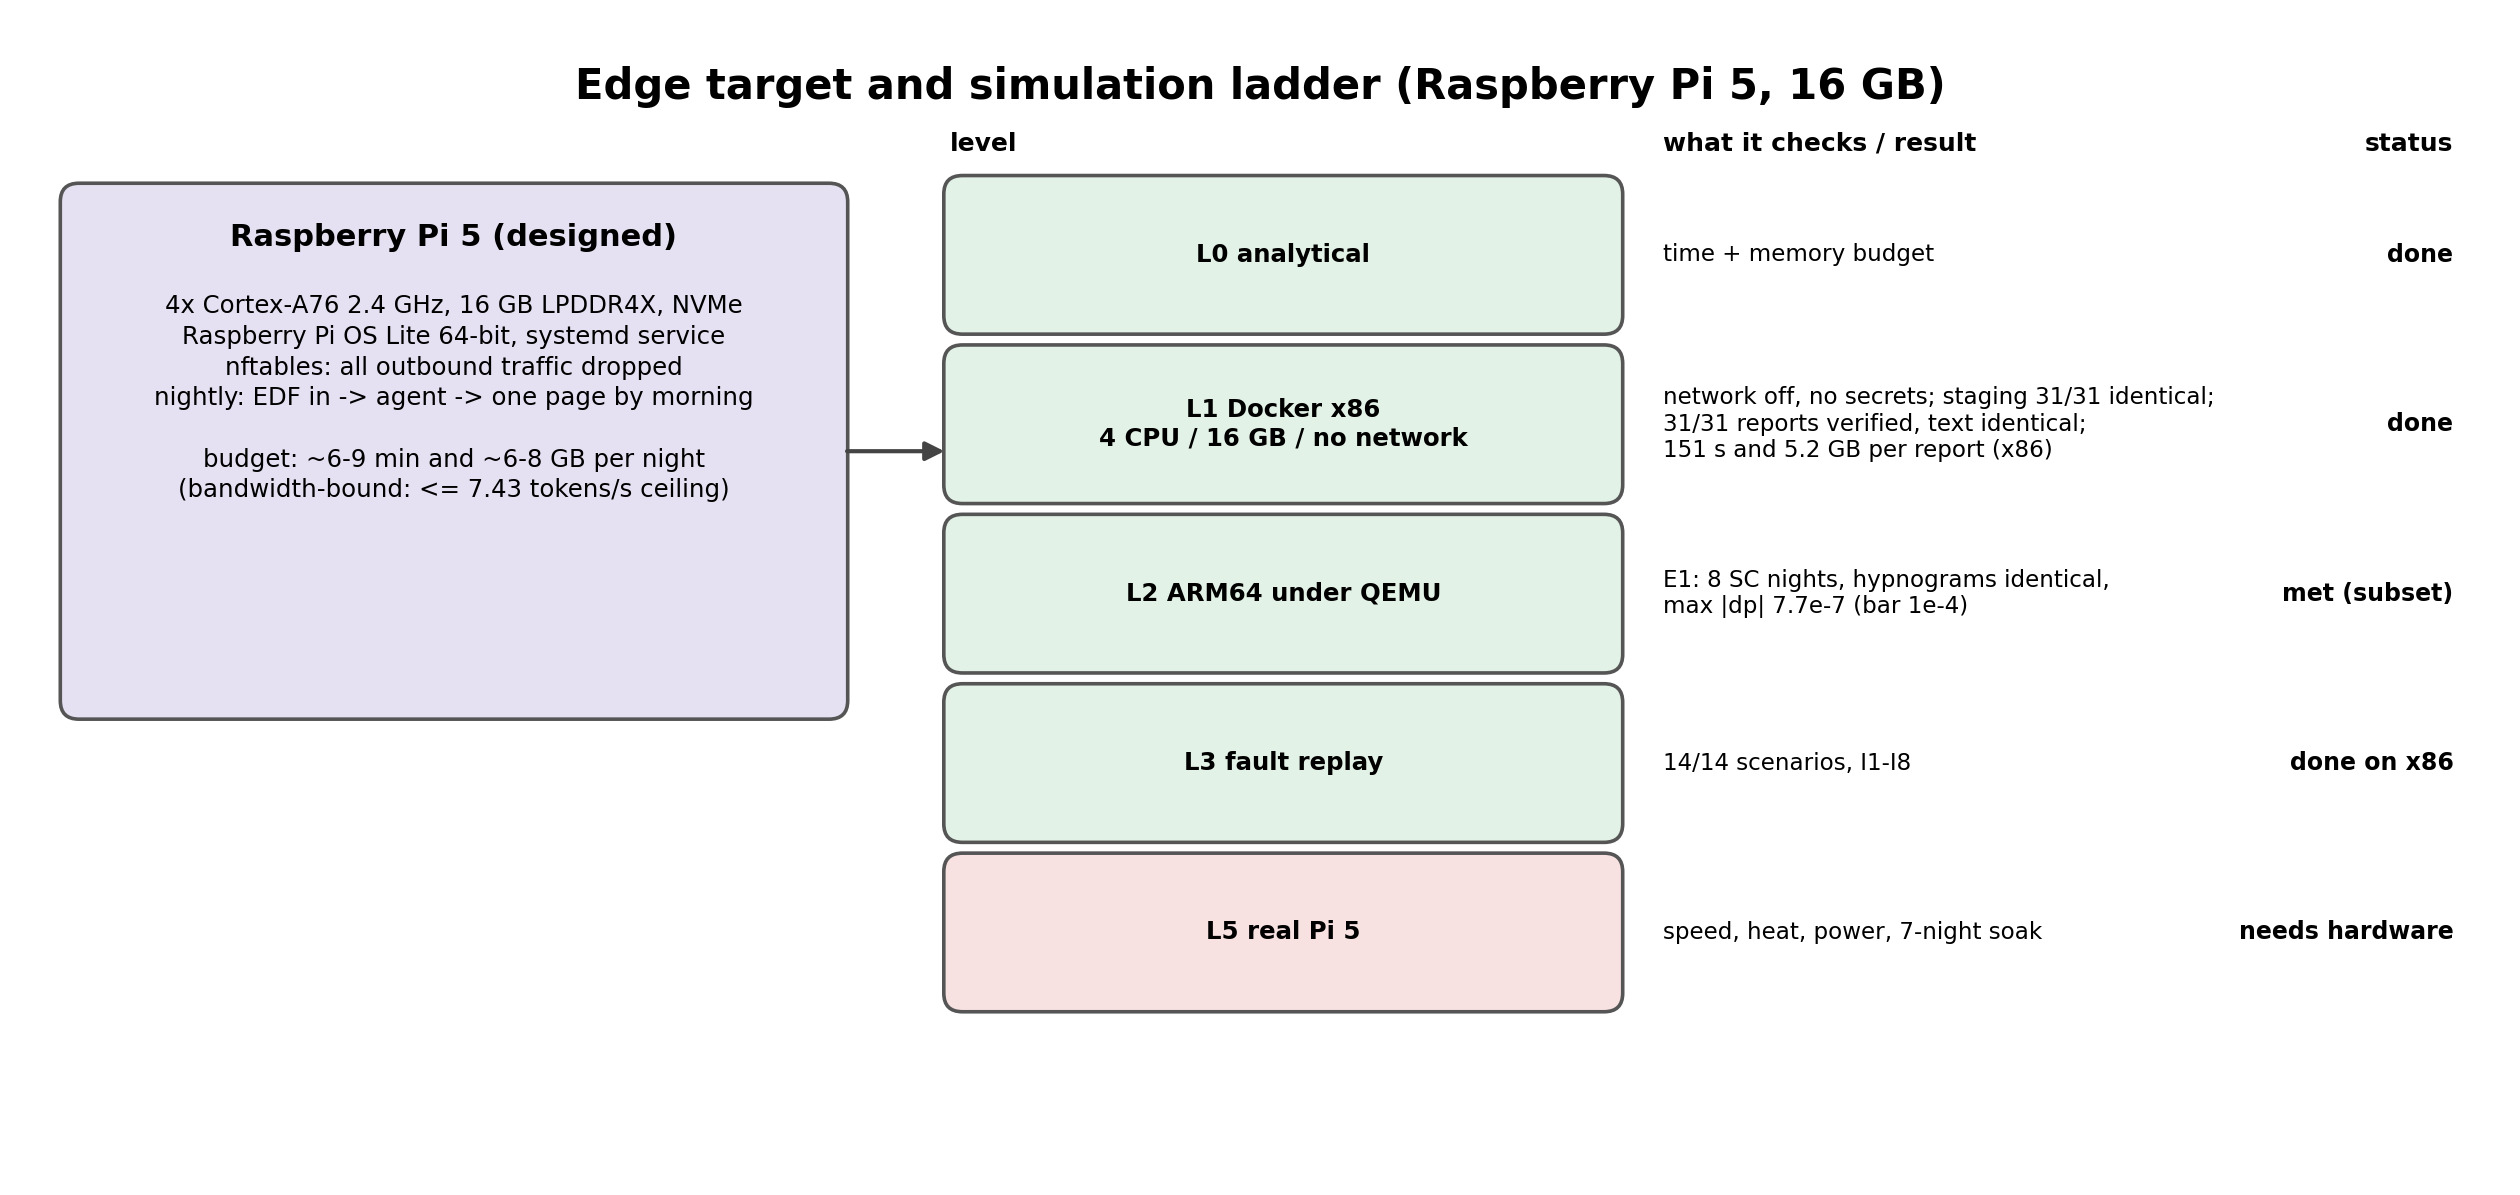
\includegraphics[width=\textwidth]{A6_edge_and_simulation.jpg}
\caption{Edge target (Raspberry Pi 5) and the simulation ladder with its current status.}
\label{fig:edge}
\end{figure}

\subsection{ Expected Outcomes}

\begin{itemize}
  \item A staging student under 200\,K parameters at or above its teacher's $\kappa$ on unseen subjects, and
  competitive on the standard benchmark.
  \item An evidence packet whose confidence signals separate good nights from bad without ground truth.
  \item A report model that, behind the verifier, releases no flawed report on held-out nights.
  \item An agent that reaches the expected outcome in every fault scenario and reproduces its outputs exactly.
  \item An edge plan that holds up in emulation: offline, secret-free, and numerically identical across platforms.
\end{itemize}

\subsection{Advantages of the Proposed Work}

\begin{itemize}
  \item \textbf{Small.} The staging model is 0.70\,MB (fp32), smaller than every published model at its accuracy
  level except LightSleepX.
  \item \textbf{Safe by construction.} The verifier compares values exactly, so a released report cannot contain a
  number that differs from the packet; a failure produces a fallback, not a wrong report.
  \item \textbf{Honest about uncertainty.} Each derived value carries its measured reliability; only 3 of 24 metrics
  are safe to state without qualification, and the report says so.
  \item \textbf{Private.} Everything runs offline; the container test confirmed no network is reachable.
  \item \textbf{Reproducible and auditable.} Every component is hash-pinned, runs are deterministic, and every run
  is traced.
  \item \textbf{Robust.} Missing EOG costs only 0.012 $\kappa$; bad signals, crashes, overheating and power loss each
  end in a defined, truthful outcome.
  \item \textbf{Swappable.} A new staging or report model is a new release file, not new agent code.
\end{itemize}

\subsection{Limitations and Assumptions}

\begin{itemize}
  \item \textbf{One dataset.} Everything rests on Sleep-EDFx. Within it, crossing from the SC to the ST cohort cost
  0.187 $\kappa$ for a v1-era model, which shows how little a single-dataset figure should be trusted to transfer.
  \item \textbf{Small evaluation sets.} 29 test nights give a 95\% lower bound of 82.2\% on 28/29. The test set has
  been read 7 times across the model line (logged, never for selection) and cannot evaluate any later model.
  \item \textbf{"Verified" means consistent with the packet}, not clinically correct. No clinician has rated a
  report, and the plain-language wording has not been tested with readers.
  \item \textbf{Label differences.} Corrected labels may differ from other papers' pipelines.
  \item \textbf{Night window.} Path~B uses the dataset's lights-off times for the device-like crop; the study-period
  end-point p90 error is 41 epochs on v2 against a 30-epoch bar (an accepted deviation). On some SC nights the
  research packets start before an evening nap, which inflates WASO; such nights are left ungraded in the
  plain-language view.
  \item \textbf{Edge numbers.} The Pi budget is analytical. Measured so far: an x86 container (timing on a desktop CPU,
  not the Pi's) and ARM64 staging parity under emulation on 8 Sleep Cassette nights. Not measured: the report model on
  ARM, Sleep Telemetry nights on ARM, and any timing, heat or power on a real Raspberry Pi 5.
  \item \textbf{The full system is not small.} The report model is 99.9\% of the footprint (2.02\,GB on disk, about
  4.7\,GB peak RAM).
\end{itemize}

\chapter{Experimentation and Result Analysis}
\label{chap.4}
This chapter reports the experiments in the order the work was done. Every number comes from a results file in the
repository (Appendix~A); release v2 numbers use the corrected labels.

\section{Experimental Setup}

\begin{itemize}
  \item \textbf{Training:} Kaggle notebooks, NVIDIA T4 GPU (16\,GiB). Each staging run took about 20 minutes; the v2
  report model's LoRA training took 169 minutes.
  \item \textbf{Inference and evaluation:} a Windows x86 PC (CPU only, about 7\,GB free RAM); llama.cpp b10927;
  Python 3 with PyTorch, MNE and SciPy.
  \item \textbf{Edge simulation (L1):} a second Windows PC with Docker Desktop; a Linux x86-64 container (Python
  3.12, CPU-only PyTorch, llama.cpp b10927 built from source) limited to 4 CPUs and 16\,GiB, started with
  \texttt{--network none} and the project mounted read-only.
  \item \textbf{Determinism:} report generation at temperature 0, seed 0, fixed grammar and pinned chat template.
  \item \textbf{Edge target (not yet measured):} Raspberry Pi 5, 4$\times$ Cortex-A76 at 2.4\,GHz, 16\,GB LPDDR4X, NVMe.
\end{itemize}

\section{Datasets:}

Sleep-EDFx as described in Section~\ref{sec:dataset}, with these evaluation configurations:
\begin{itemize}
  \item \textbf{Held-out test:} 15 subjects, 29 nights, 33,365 epochs; locked, one logged read per model.
  \item \textbf{Standard benchmark (B1):} Sleep-EDF-78 (SC only, 78 subjects, 153 nights), 10-fold subject-wise
  cross-validation, trained from scratch (no warm start, no distillation); 78/78 subjects and 153/153 recordings
  each appear in exactly one fold.
  \item \textbf{Cohort transfer:} train on 62 SC subjects, test on all 22 ST subjects.
  \item \textbf{Path B (raw EDF):} the 31 dev nights cropped at lights-off to a 12-hour device-like window, with no
  expert hypnogram; the study period is estimated by the model.
  \item \textbf{Report model:} 123 training and 14 validation nights with reference targets; 31 dev nights for
  selection; the 29 test nights once (pre-registered).
\end{itemize}

\section{Evaluation Metrics:}

\begin{itemize}
  \item \textbf{Staging:} accuracy; \textbf{Cohen's $\kappa$} (primary, robust to class imbalance); macro-F1 and
  per-class F1; bootstrap 95\% CIs resampled \emph{by subject}; paired Wilcoxon signed-rank tests per subject.
  \item \textbf{Calibration:} expected calibration error (ECE, 15 bins); night-level Pearson / Spearman correlation
  between mean entropy and $\kappa$.
  \item \textbf{Reports:} verified (no violation); \textbf{5/5} (verified and all mandatory items covered);
  violations; \textbf{numeric fidelity} (cited values equal to packet values); flawed reports released; two-sided
  95\% Clopper--Pearson lower bound (for $n/n$ successes, $0.025^{1/n}$).
  \item \textbf{Agent:} outcome and reason codes per scenario; invariants I1--I8; byte-identical reruns; wall time.
  \item \textbf{Edge:} network reachability, secret scan, cross-platform staging parity (max $|\Delta p|$, identical
  hypnograms), wall time and peak memory per night; tokens/s (analytical for the Pi).
\end{itemize}

\section{Experimental Design}

\textbf{Baseline methods:} the inherited 649,229-parameter model (re-evaluated honestly); retrained teachers E0,
E1a, E1b; a non-distilled student of the same size (the control for every KD experiment); the v1 student N4kd;
YASA 0.8.1; the published models of Table~\ref{tab:published}; and, for reports, five untrained small models and
the untrained Llama-3.2-3B.

\subsection{Experimental Scenarios:}

\begin{enumerate}
  \item \textbf{Exposure gradient:} the inherited model on epochs it trained on, on the same subject's other night,
  and on an unseen subject.
  \item \textbf{KD vs control:} students distilled from teachers of different quality against an identical student
  trained on hard labels only.
  \item \textbf{Encoder and channel ablations:} receptive field, raw EEG zeroed, EOG added.
  \item \textbf{Architecture ablation (5-fold CV, same labels):} \texttt{base} $\rightarrow$ \texttt{full\_eeg} (TF +
  local context + recipe) $\rightarrow$ \texttt{full} (+ EOG).
  \item \textbf{Missing channel:} v2 evaluated with the EOG input removed.
  \item \textbf{Report-model selection:} reference run, grammar ablation, LoRA students on dev, one test run.
  \item \textbf{Verifier ablation:} gate on / gate off / gate and grammar off, on 31 dev nights, for v1, v2 and the
  untrained model.
  \item \textbf{Agent fault scenarios:} 15 scenarios on real EDF files and injected report-model faults.
  \item \textbf{Sampling rates and line noise:} 128 and 256\,Hz recordings; 49/50\,Hz noise injected at 0.25--2$\times$
  EEG RMS.
  \item \textbf{Reproducibility:} Path B twice per dev night in fresh runtime directories with the real model.
  \item \textbf{Edge containers:} environment checks; staging on all 31 dev recordings; the report model on all 31
  dev packets; three raw nights end to end; and staging on 8 nights under ARM64 emulation --- all inside offline,
  resource-limited containers and compared with the reference PC.
\end{enumerate}

\subsection{Parameter Tuning:}

\begin{itemize}
  \item Distillation: $\alpha = 0.5$, $T = 3$, fixed for every reported run.
  \item Staging: AdamW, lr $3\times10^{-4}$, 75 epochs, model selection on \textbf{validation} macro-F1; 3 seeds for v2.
  \item Calibration temperature, decoder, night-confidence tiers and the N1 flag threshold: fitted on validation
  only, applied unchanged to test.
  \item Report model: hyperparameters pre-registered and locked before training (Table~\ref{tab:sft}).
  \item Agent thresholds (quality, study period, resources): set in the policy file and calibrated on train/dev.
\end{itemize}

\begin{table}[htbp]
\centering\small
\caption{Report-model training configuration (identical for v1 and v2).}
\label{tab:sft}
\begin{tabularx}{\textwidth}{lY}
\toprule
Parameter & Value \\
\midrule
Base models & Llama-3.2-3B-Instruct; Qwen2.5-1.5B-Instruct \\
Method & LoRA (PEFT), rank 16, $\alpha$ 32, dropout 0.05, on q/k/v/o and MLP projections \\
Optimiser & lr $2\times10^{-4}$, cosine; effective batch 8; 3 epochs; seed 0 \\
Data & 123 training nights, 14 validation nights; targets = reference claim sets that pass the verifier, serialised in the grammar's field order \\
Max sequence & 3,072 tokens \\
Export & F16 $\rightarrow$ Q4\_K\_M with llama.cpp b10927 \\
\bottomrule
\end{tabularx}
\end{table}

\section{Results}

\subsection{Stage 1 --- Knowledge distillation (v1, stored labels, historical)}\label{sec:res-kd}

\textbf{The inherited model had memorised people} (Table~\ref{tab:exposure}, Figure~\ref{fig:exposure}). Its
reported $\kappa$ of 0.6663 is reproduced to within 0.0008 as a blend of the leaked and clean measurements,
confirming leakage as the explanation.

\begin{table}[htbp]
\centering\small
\caption{Exposure gradient of the inherited model.}
\label{tab:exposure}
\begin{tabular}{lrrrr}
\toprule
Exposure level & $\kappa$ & Macro-F1 & N3 F1 & REM F1 \\
\midrule
Same recording (trained on) & 0.8058 & 0.8036 & 0.889 & 0.876 \\
Same subject, other night (leaked) & 0.6797 & 0.7173 & 0.837 & 0.718 \\
\textbf{Unseen subject} & \textbf{0.5066} & \textbf{0.4107} & \textbf{0.000} & \textbf{0.184} \\
\bottomrule
\end{tabular}
\end{table}

\begin{figure}[htbp]
\centering
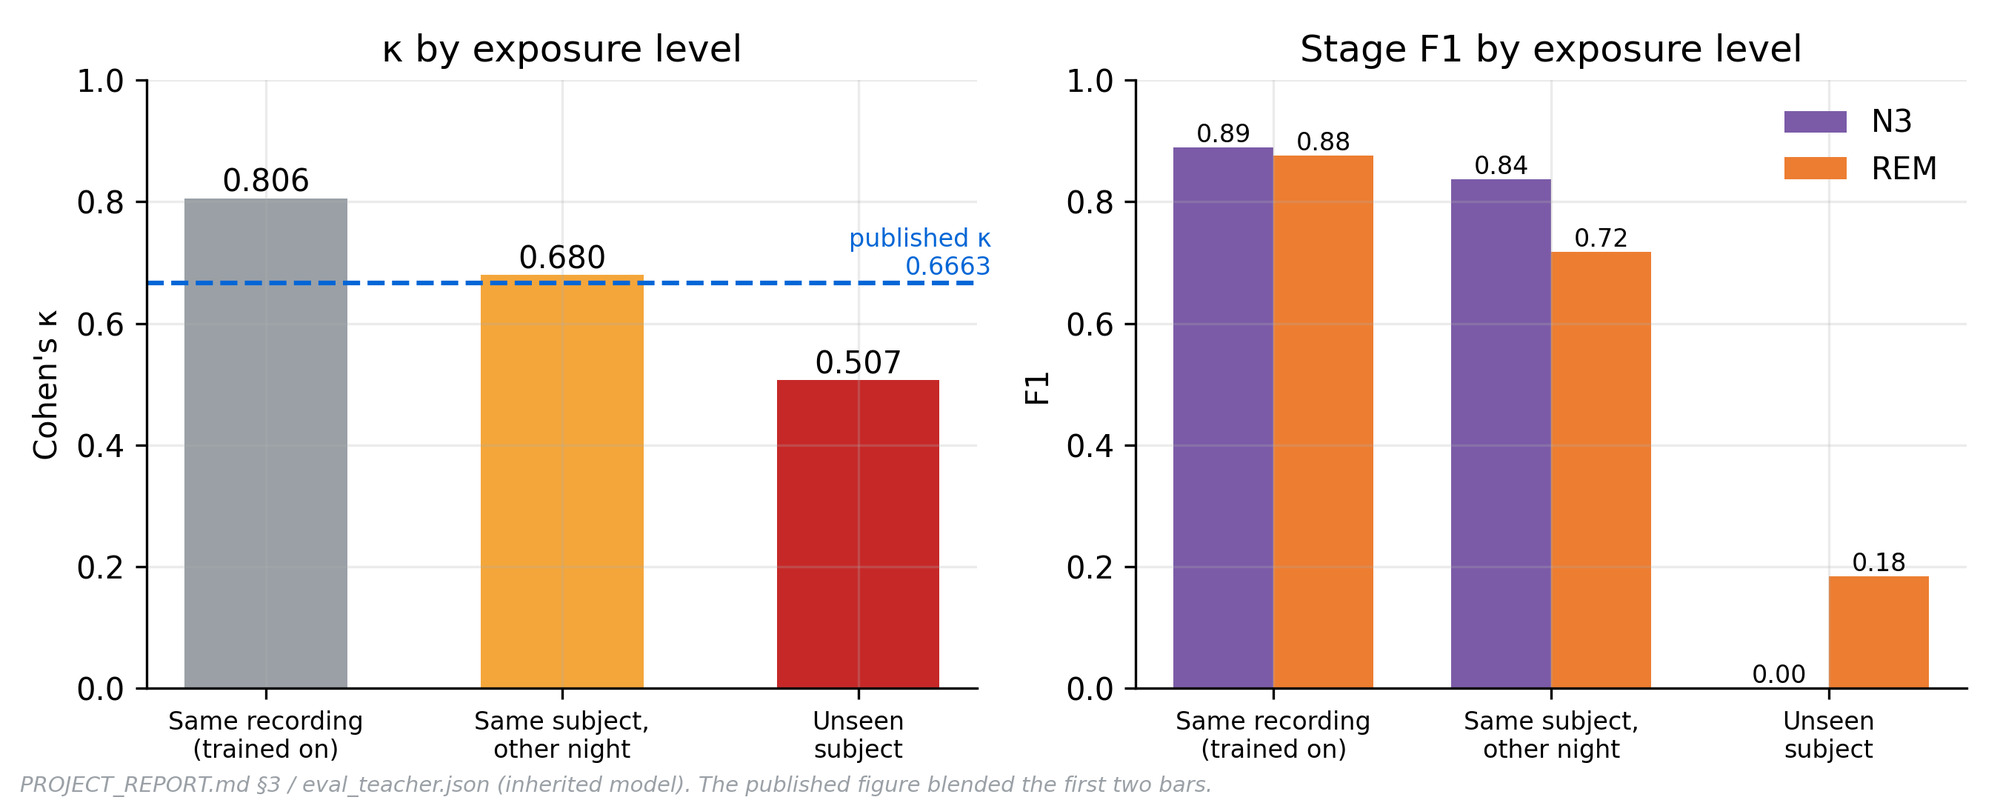
\includegraphics[width=0.8\textwidth]{F3_exposure_gradient.jpg}
\caption{Exposure gradient: what the inherited model had memorised.}
\label{fig:exposure}
\end{figure}

\begin{table}[htbp]
\centering\small
\caption{Distillation experiments, held-out test (15 subjects), stored labels (v1 era).}
\label{tab:kd}
\begin{tabular}{lrrr}
\toprule
Model & Params & $\kappa$ & Macro-F1 \\
\midrule
E0 teacher (faithful retrain) & 649,229 & 0.5122 & 0.6063 \\
E1b teacher (double class-weighting fixed) & 649,229 & 0.6055 & 0.6548 \\
Student distilled from E0 & 121,099 & 0.5925 & 0.6611 \\
Student distilled from E1b & 121,099 & 0.6134 & 0.6708 \\
\textbf{Student, no distillation (control)} & 121,099 & \textbf{0.6449} & \textbf{0.6915} \\
Student, multi-scale encoder & 139,606 & 0.6992 & 0.7407 \\
Ensemble teacher (3 students) & 412,311 & 0.7140 & 0.7542 \\
Student distilled from the ensemble (v1, N4kd) & 139,606 & 0.7001 & 0.7376 \\
\bottomrule
\end{tabular}
\end{table}

\textbf{Findings} (Table~\ref{tab:kd}):
\begin{enumerate}
  \item \textbf{Fixing the teacher's loss mattered more than capacity.} E1a's focal loss applied class weights twice,
  suppressing N2; fixing it (E1b) raised test $\kappa$ from 0.559 to 0.606 with no added parameters
  (Figure~\ref{fig:ladder}).
  \item \textbf{Naive KD hurt.} Both distilled students scored below the control, significantly. The student had
  outgrown its teacher during training, so half of every gradient pulled a good model towards a worse one
  (Figures~\ref{fig:kdmech} and~\ref{fig:penalty}). \emph{A teacher must exceed the student's own undistilled
  performance before its soft targets carry usable information}; no choice of $\alpha$ or $T$ can fix this.
  \item \textbf{The encoder could not see sleep.} Its receptive field was 0.25\,s, too short for any sleep
  microstructure. Widening it to 8.75\,s moved the raw EEG from contributing nothing to driving 71\% of predictions
  and raised N1 F1 by 0.092.
  \item \textbf{An ensemble of comparable, diverse students is a teacher that works.} It exceeds each member, and
  distilling it removed the penalty. On accuracy the distilled student tied its hard-label twin; what improved was
  \textbf{calibration}: ECE fell by about a third and REM-latency error nearly halved (Figure~\ref{fig:calib}).
  \item \textbf{The evaluation became the limit.} 5-fold subject-level CV showed the original validation split was
  an unrepresentative draw ($\kappa$ 0.7143 across folds vs 0.6763 on that split; fold SD 0.0193), larger than the
  whole distillation effect on $\kappa$ (0.0008).
\end{enumerate}

\begin{figure}[htbp]
\centering
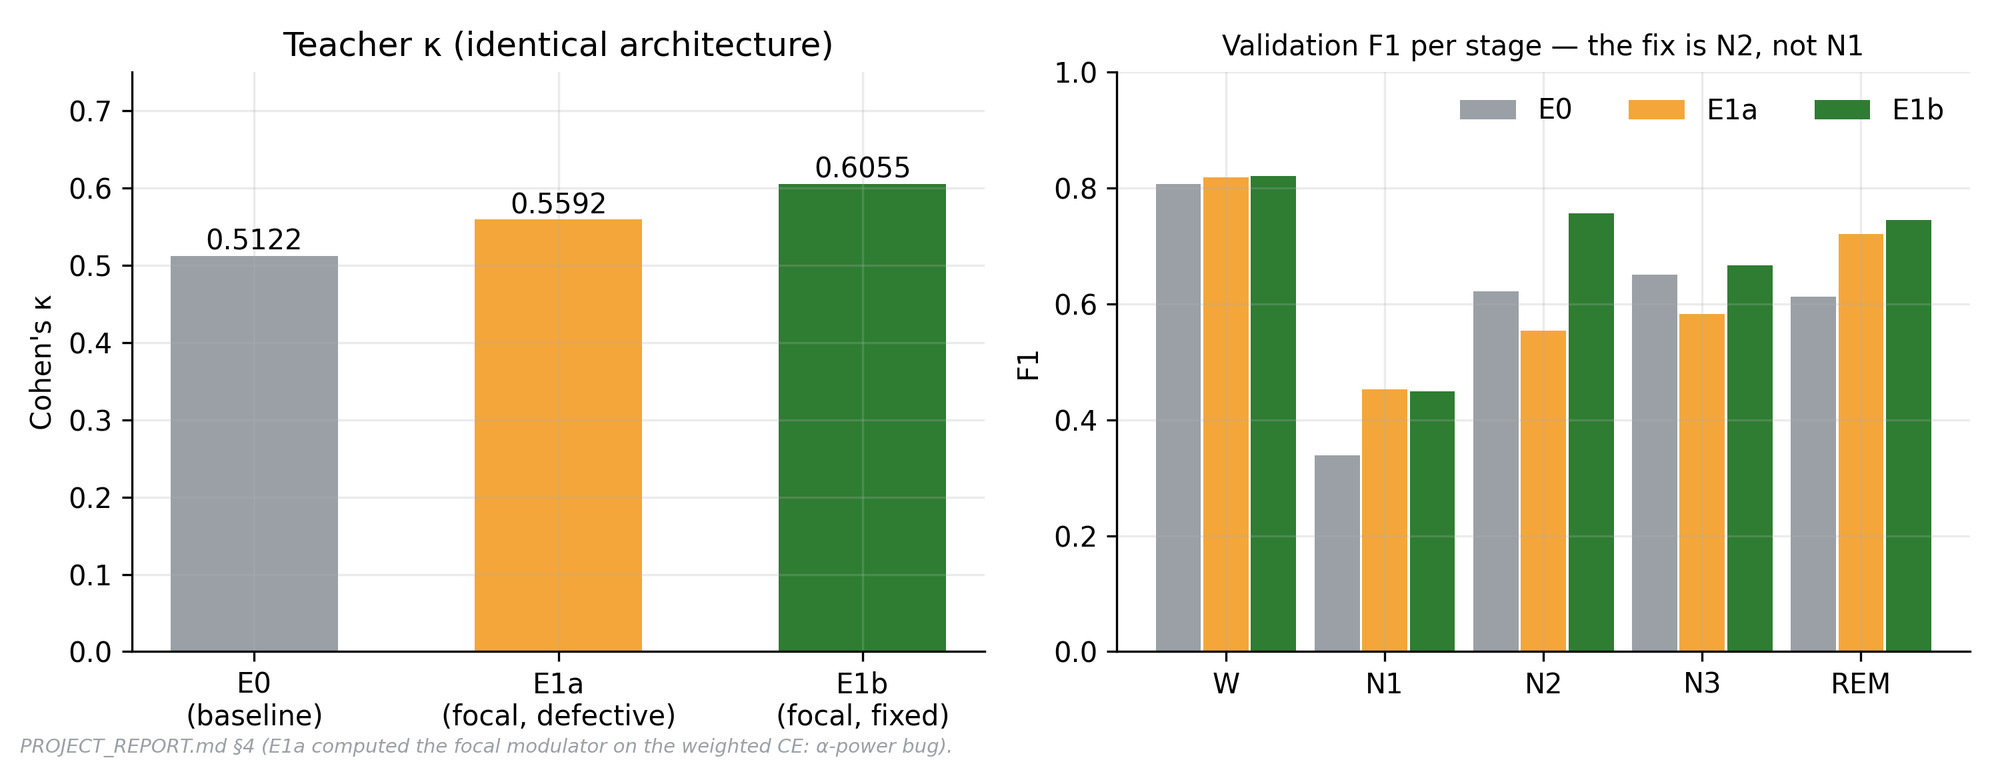
\includegraphics[width=0.75\textwidth]{v1_F6_teacher_ladder.jpg}
\caption{Teacher ladder E0 $\rightarrow$ E1a $\rightarrow$ E1b (v1 era, stored labels).}
\label{fig:ladder}
\end{figure}

\begin{figure}[htbp]
\centering
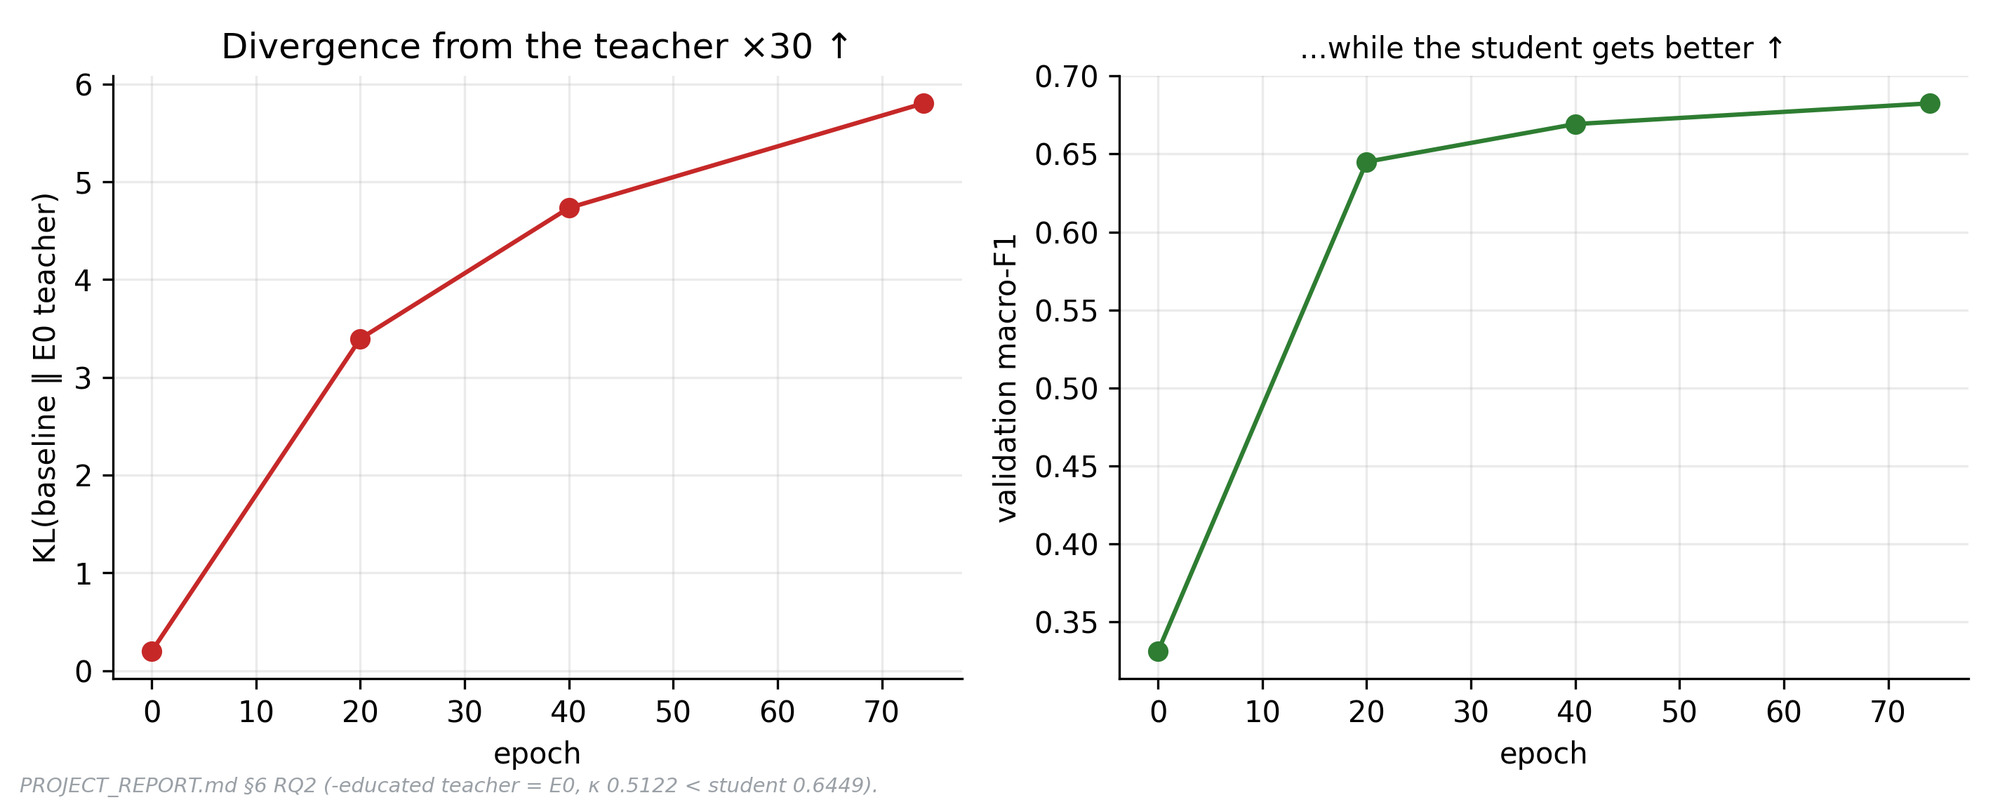
\includegraphics[width=0.85\textwidth]{v1_F11_kd_mechanism.jpg}
\caption{Why single-teacher distillation failed: the distillation mechanism.}
\label{fig:kdmech}
\end{figure}

\begin{figure}[htbp]
\centering
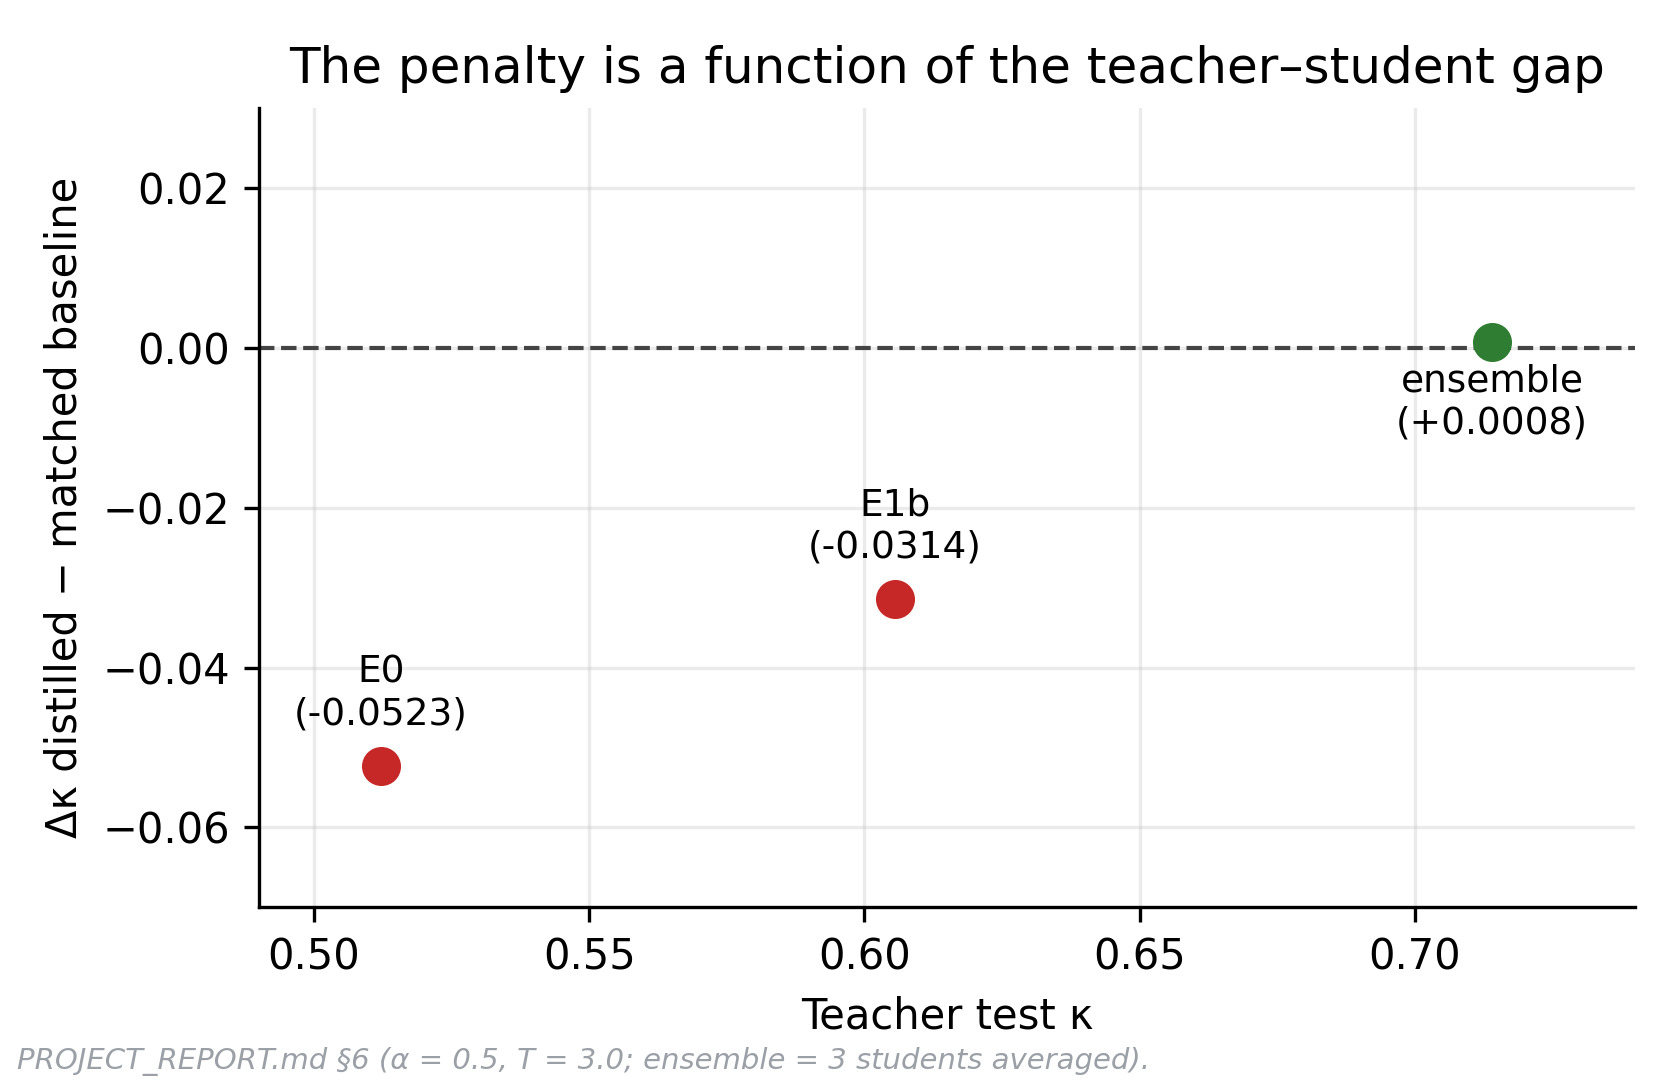
\includegraphics[width=0.7\textwidth]{v1_F12_penalty_vs_teacher.jpg}
\caption{Distillation penalty against teacher quality.}
\label{fig:penalty}
\end{figure}

\begin{figure}[htbp]
\centering
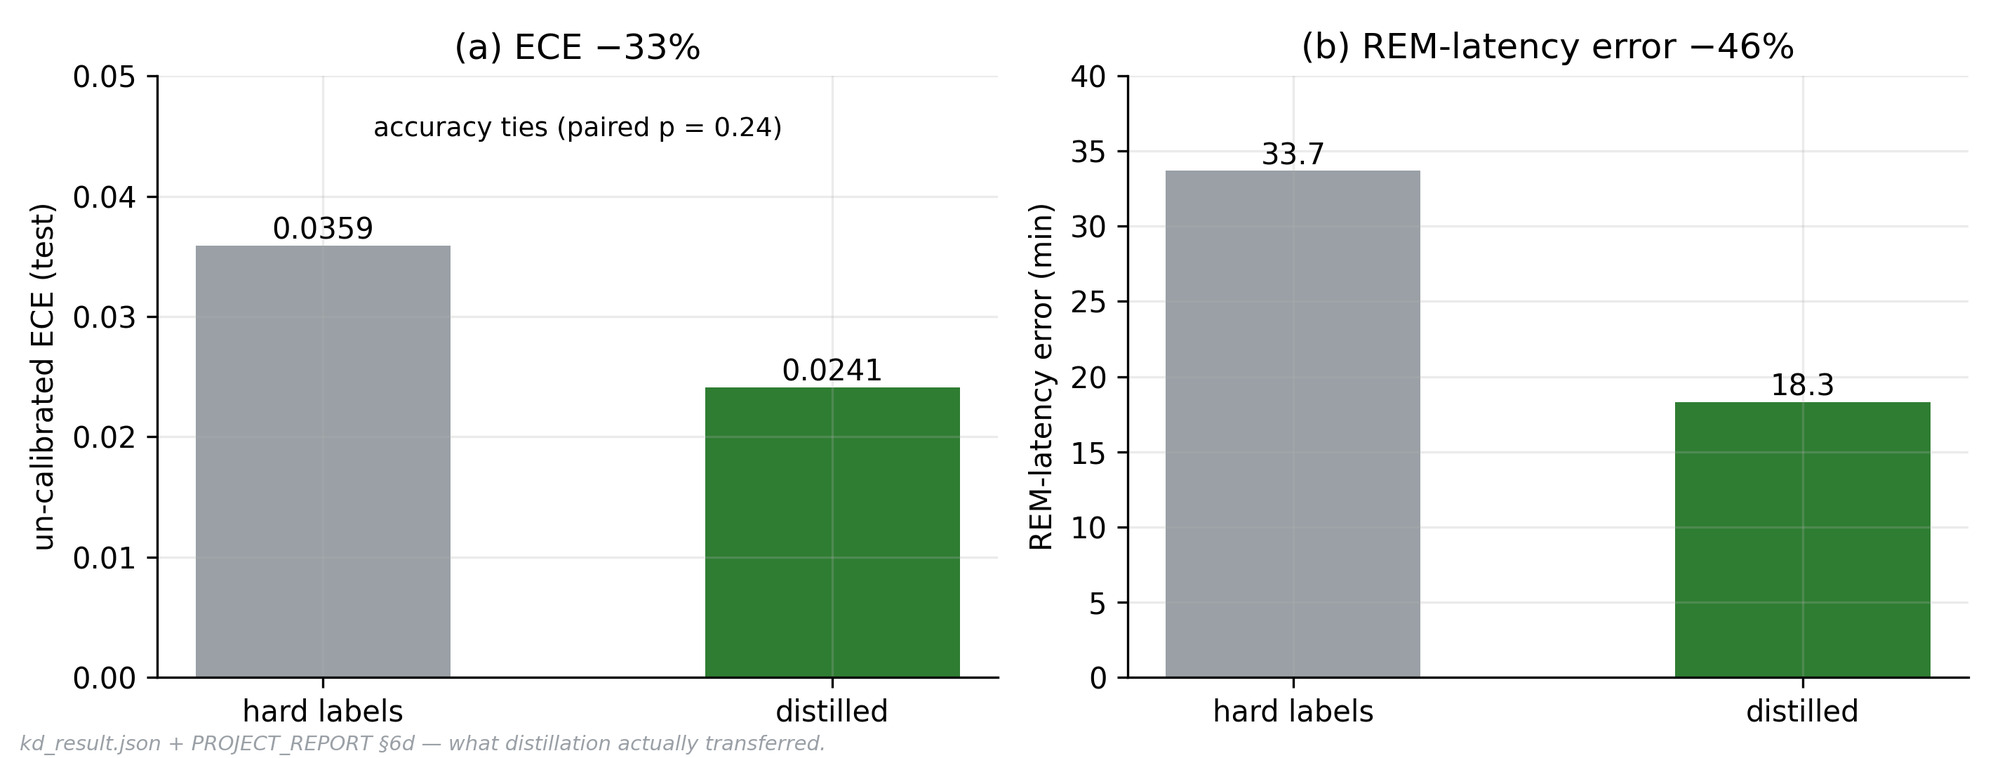
\includegraphics[width=0.85\textwidth]{v1_F13_calibration_transfer.jpg}
\caption{Calibration transfer through distillation.}
\label{fig:calib}
\end{figure}

\subsection{Stage 2 --- Student model (release v2, corrected labels)}

\begin{table}[htbp]
\centering\small
\caption{Held-out test, 15 subjects, 29 nights, 33,365 epochs, corrected labels.}
\label{tab:v2test}
\begin{tabular}{lrlrrrrr}
\toprule
Model & Params & Input & Acc. & $\kappa$ & MF1 & N1 F1 & REM F1 \\
\midrule
ENSmc teacher & 412,311 & EEG & 80.02\% & 0.732 & 76.91 & 48.7 & 81.8 \\
v1 student (N4kd) & 139,606 & EEG & 79.00\% & 0.718 & 75.23 & 45.5 & 78.2 \\
\textbf{v2 student (N6adv)} & \textbf{175,599} & \textbf{EEG + EOG} & \textbf{81.96\%} & \textbf{0.756} & \textbf{78.20} & \textbf{50.7} & \textbf{83.7} \\
v2, EOG removed & 175,599 & EEG & 81.10\% & 0.744 & 77.20 & 48.7 & -- \\
\bottomrule
\end{tabular}
\end{table}

\begin{itemize}
  \item v2 vs v1 (Table~\ref{tab:v2test}): $\Delta\kappa$ +0.038, 95\% CI [+0.019, +0.057]; better on 13/15
  subjects (Wilcoxon $p = 0.0009$); every stage improves (W +0.7, N1 +5.3, N2 +2.4, N3 +1.0, REM +5.3 F1 points).
  Accuracy passes 80\% on both cohorts (SC 82.1\%, ST 81.4\%).
  \item v2 beats its teacher on every metric with 43\% of its parameters. This test comparison combines label
  correction, EOG and the training recipe; the like-for-like attribution is the ablation in Table~\ref{tab:ablation}.
\end{itemize}

\begin{table}[htbp]
\centering\small
\caption{Architecture ablation, 5-fold CV, corrected labels for every arm.}
\label{tab:ablation}
\begin{tabular}{lrrl}
\toprule
Arm & Params & $\kappa$ & $\Delta\kappa$ vs base, 95\% CI \\
\midrule
\texttt{base} (v1 architecture) & 139,606 & 0.7584 & -- \\
\texttt{full\_eeg} (+ TF branch, local context, recipe) & 160,511 & 0.7653 & +0.0069 [+0.003, +0.011] \\
\textbf{\texttt{full} (+ EOG) = v2} & \textbf{175,599} & \textbf{0.7763} & \textbf{+0.0179 [+0.0095, +0.026]}, 5/5 folds \\
\bottomrule
\end{tabular}
\end{table}

\begin{figure}[htbp]
\centering
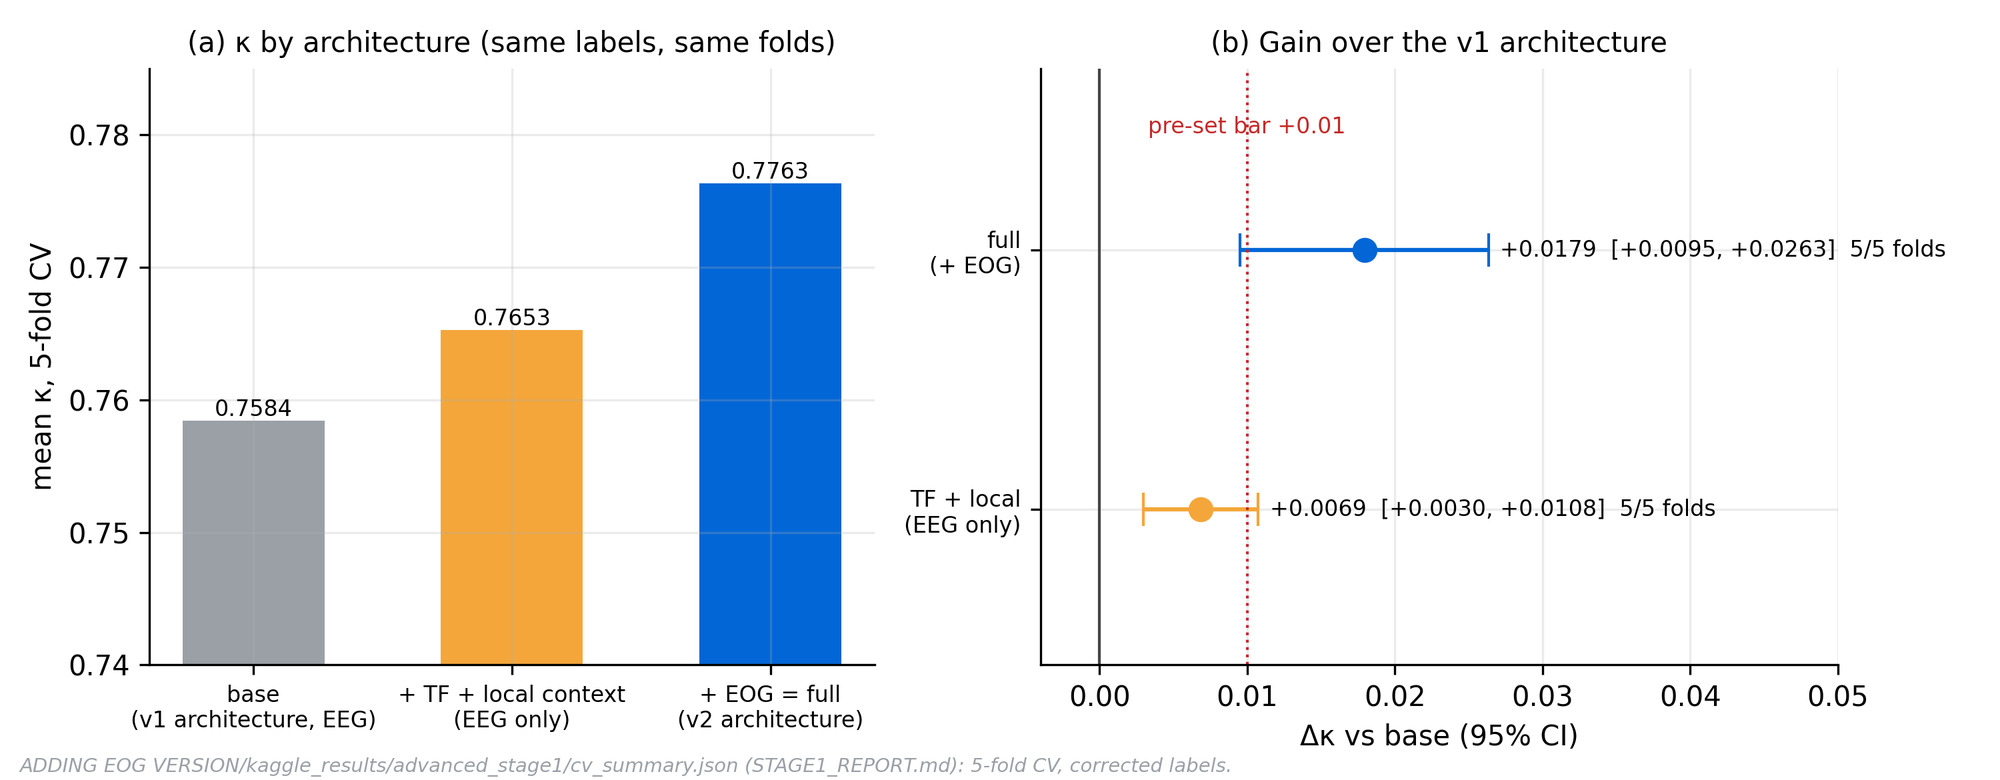
\includegraphics[width=0.85\textwidth]{F26_architecture_ablation.jpg}
\caption{Architecture ablation: what the time-frequency branch, local context and EOG add, like for like.}
\label{fig:ablation}
\end{figure}

\begin{figure}[htbp]
\centering
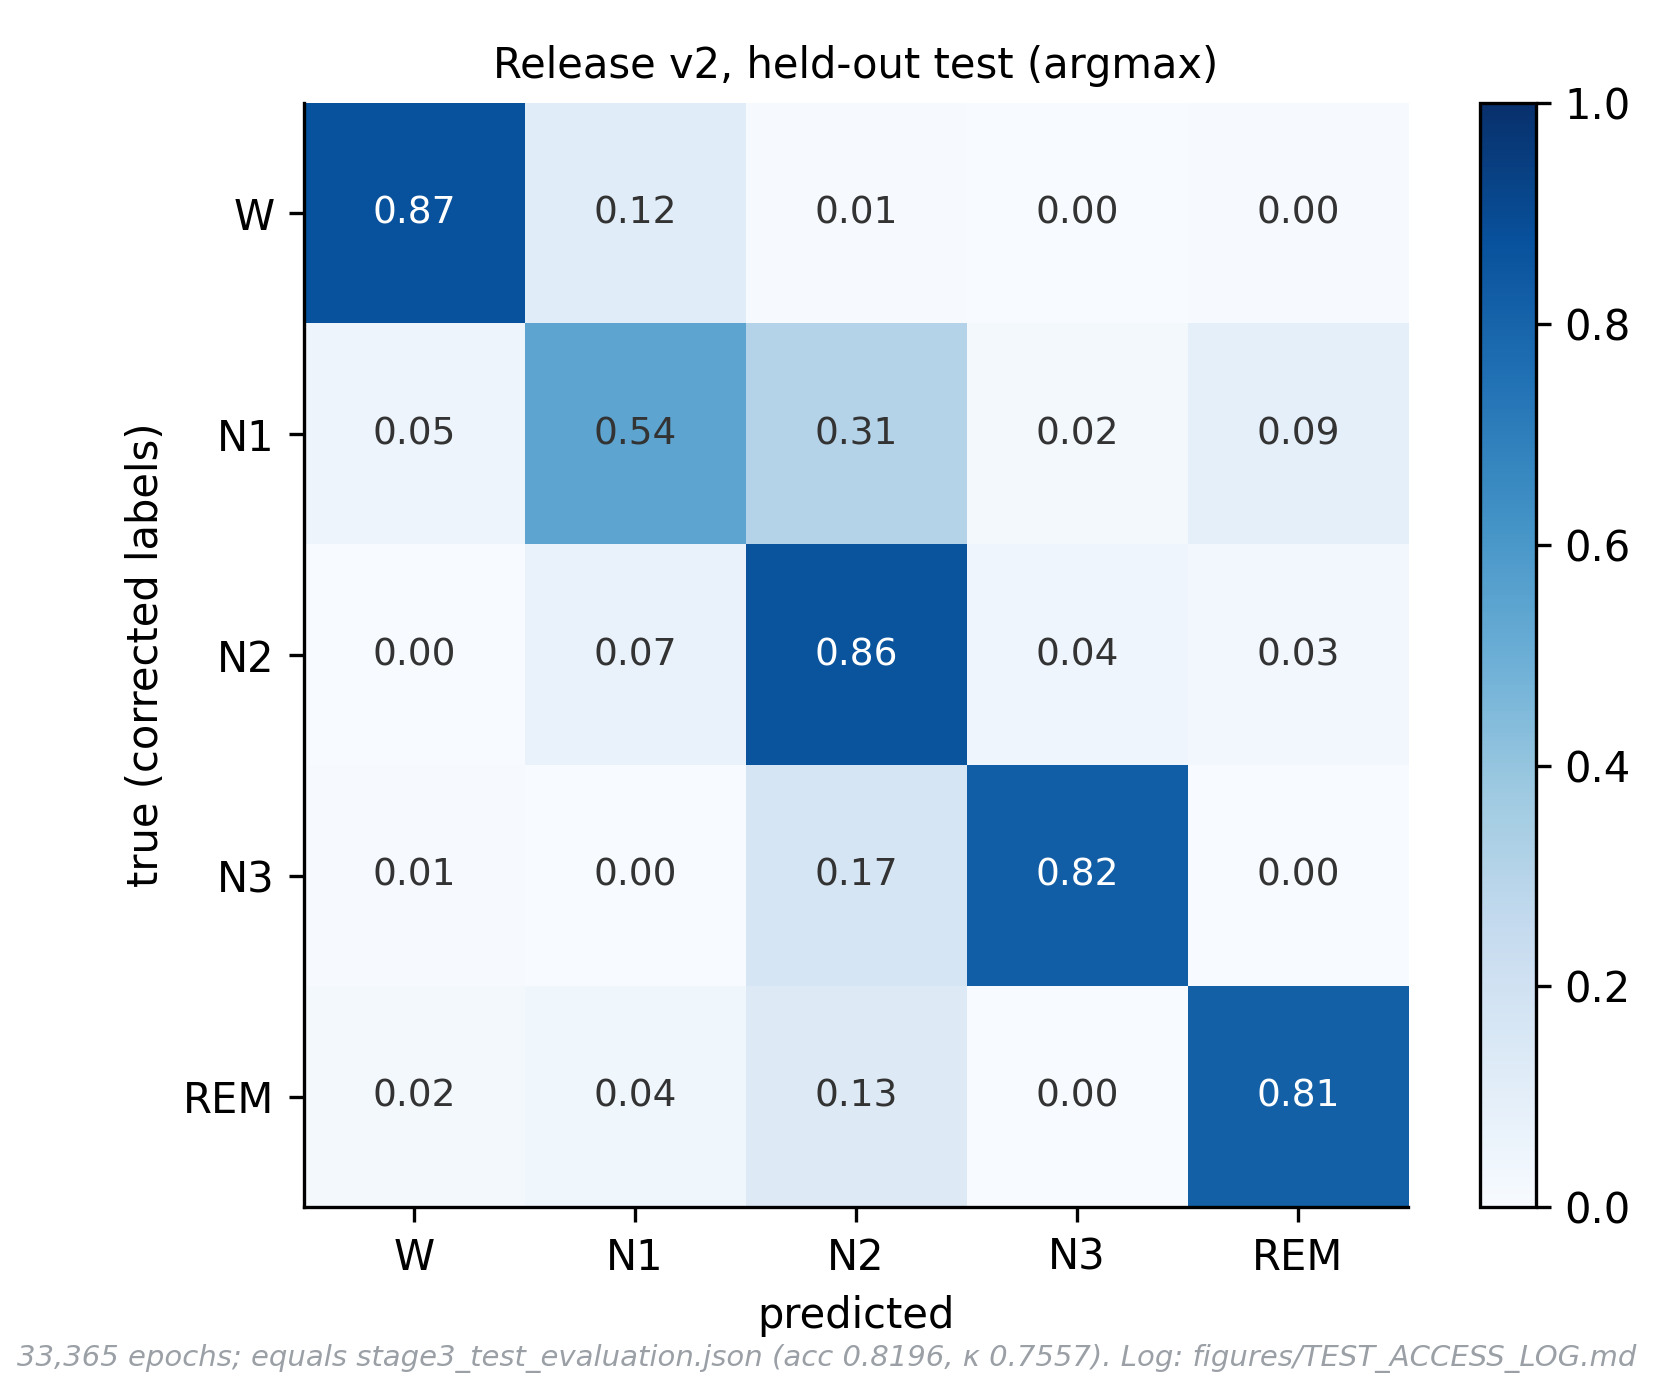
\includegraphics[width=0.75\textwidth]{F15_confusion_matrix.jpg}
\caption{Confusion matrix of release v2 on the held-out test set (corrected labels).}
\label{fig:cm}
\end{figure}

\begin{figure}[htbp]
\centering
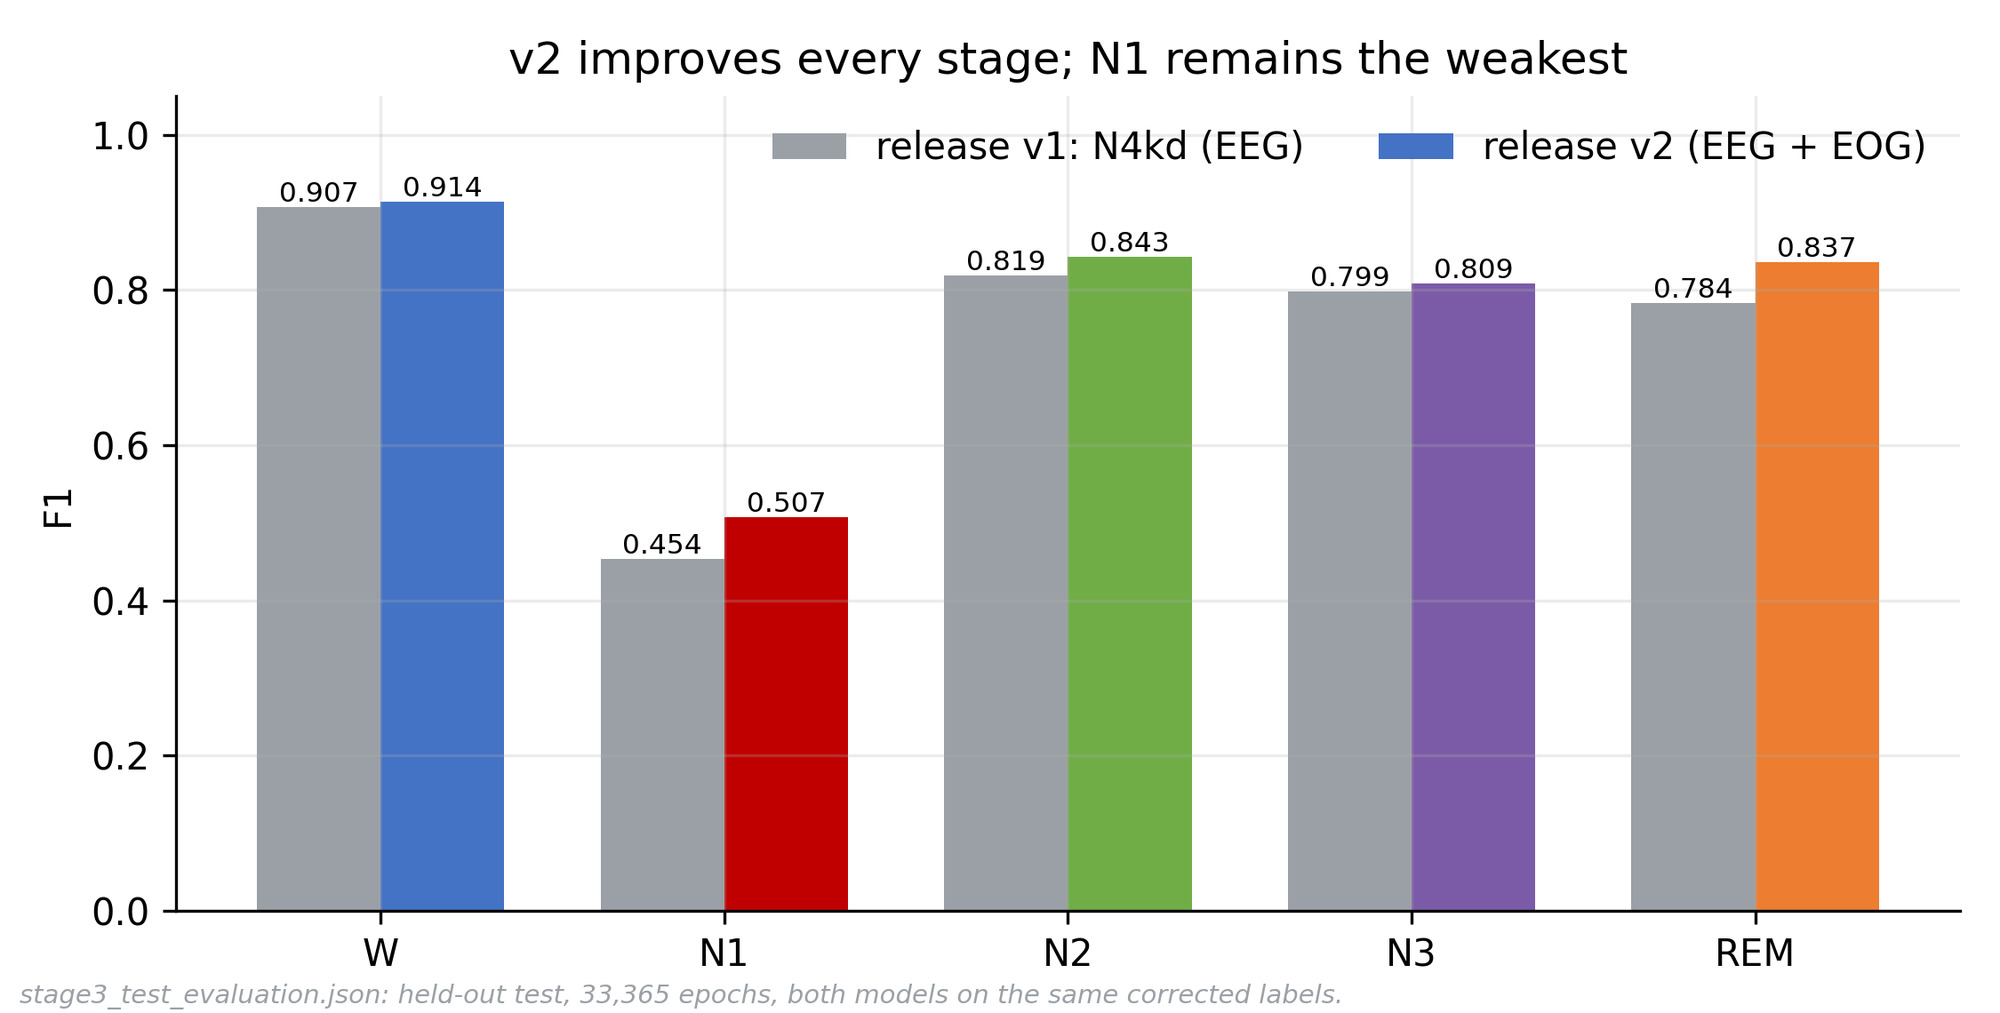
\includegraphics[width=0.85\textwidth]{F16_per_class_f1.jpg}
\caption{Per-class F1, v2 against v1 on the same labels: v2 is better on all five stages.}
\label{fig:perclass}
\end{figure}

\begin{figure}[htbp]
\centering
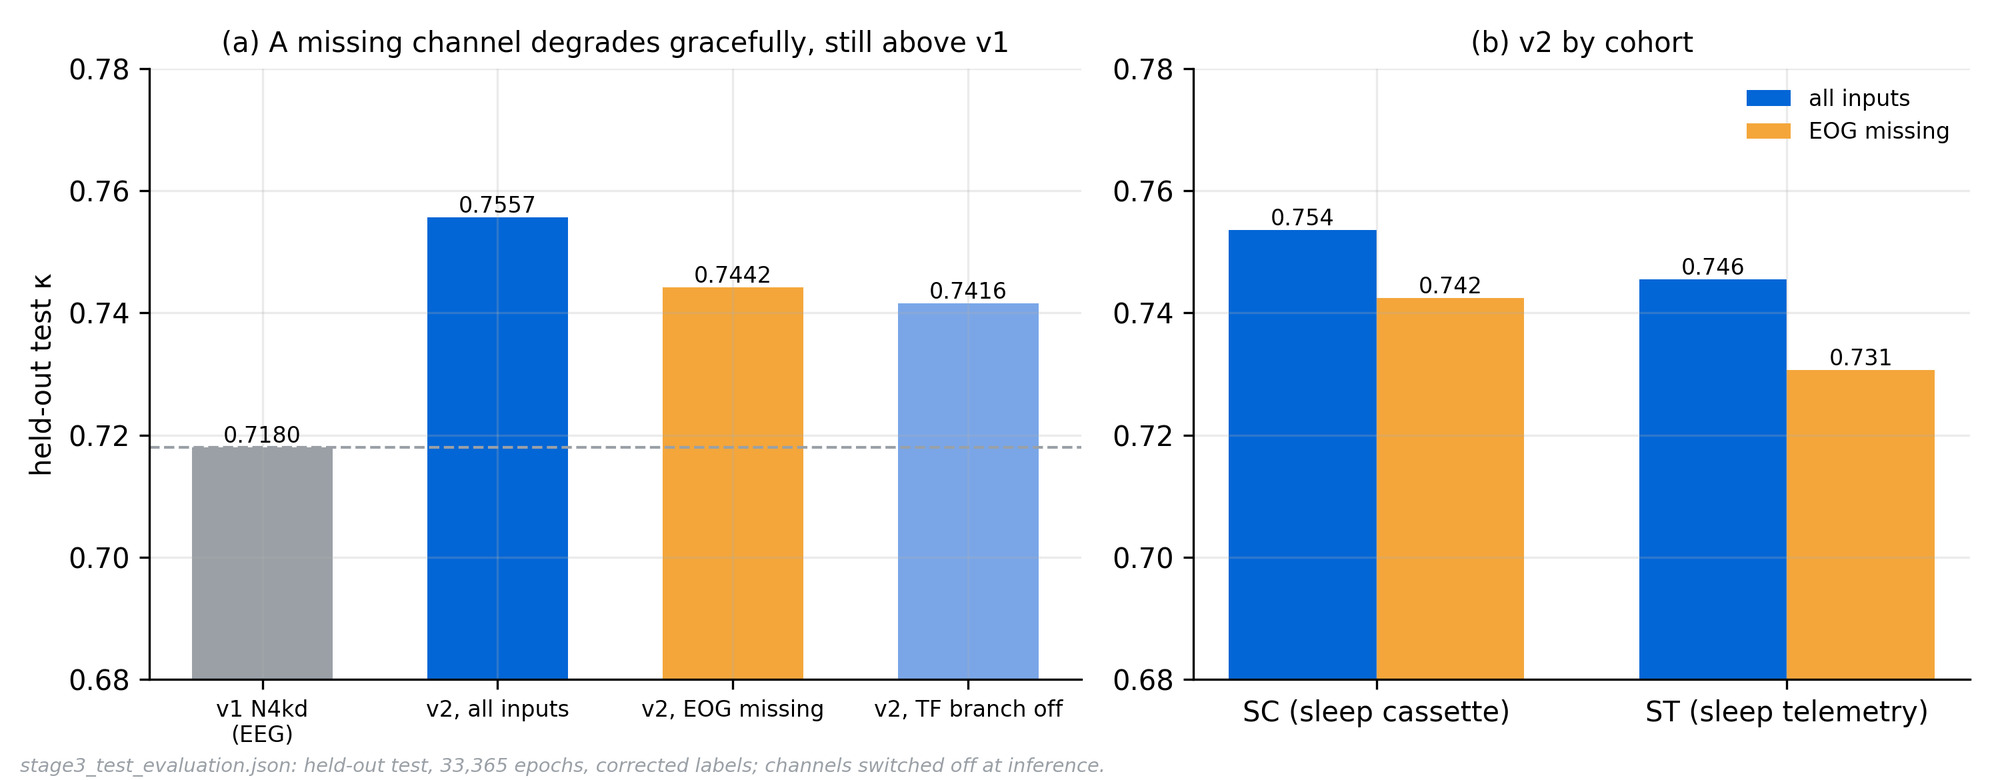
\includegraphics[width=0.85\textwidth]{F27_missing_channel_robustness.jpg}
\caption{Robustness to a missing EOG channel: 0.756 $\rightarrow$ 0.744, still above v1 (0.718).}
\label{fig:missing}
\end{figure}

\begin{table}[htbp]
\centering\small
\caption{Standard benchmark B1 (Sleep-EDF-78, 10-fold subject-wise, trained from scratch).}
\label{tab:b1}
\begin{tabular}{lrrrrrrrr}
\toprule
Aggregation & Acc. & $\kappa$ & MF1 & W & N1 & N2 & N3 & REM \\
\midrule
Final epoch, pooled (conservative) & 83.0\% & \textbf{0.769} & 78.4 & 92.7 & 51.6 & 84.3 & 77.8 & 85.7 \\
Selected epoch (optimistic) & 83.5\% & 0.775 & 79.0 & 92.9 & 53.1 & 84.7 & 78.3 & 85.9 \\
Per-recording mean & 83.2\% & 0.761 & 73.7 & -- & 52.5 & -- & -- & -- \\
\bottomrule
\end{tabular}
\end{table}

The project's own 5-fold CV ($\kappa$ 0.776) and B1 (0.775 at the selected epoch) used different folds, subjects
and training starts and agree within 0.001 $\kappa$ (Table~\ref{tab:b1}, Figure~\ref{fig:b1folds}).

\begin{figure}[htbp]
\centering
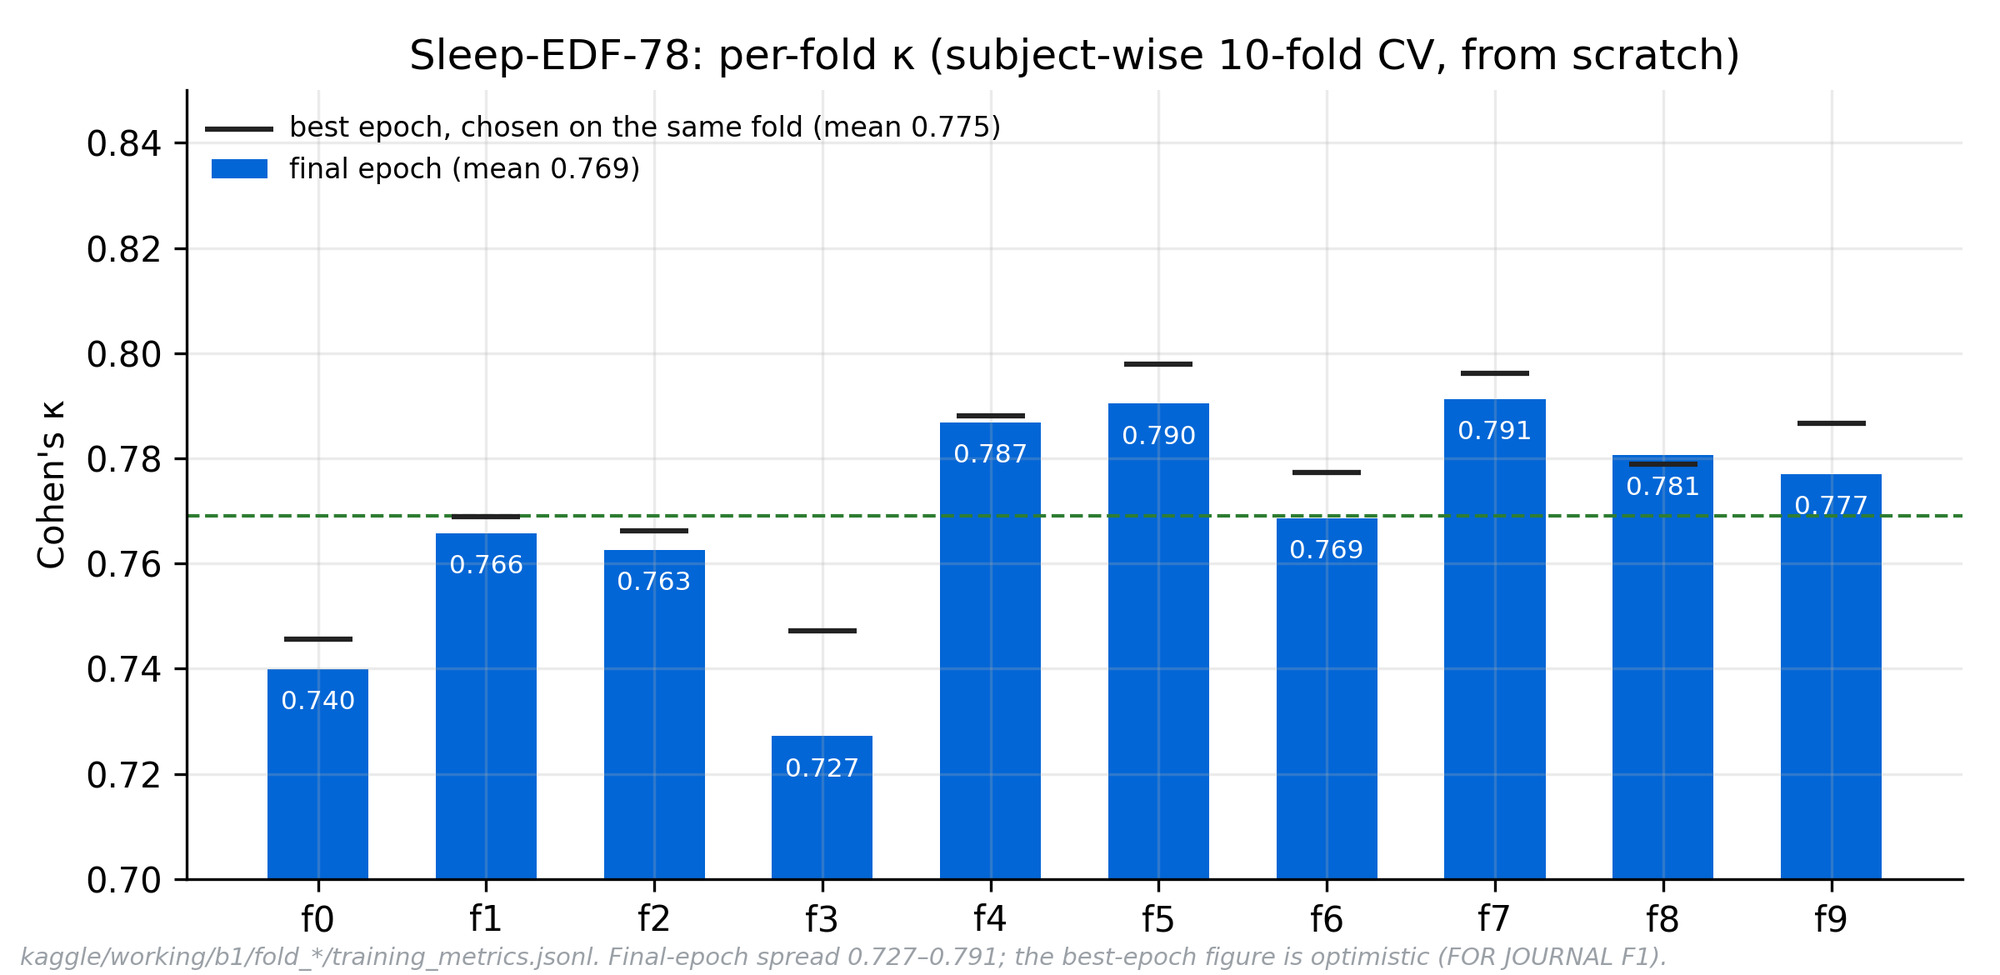
\includegraphics[width=0.85\textwidth]{F17_b1_folds.jpg}
\caption{B1 per-fold $\kappa$ (bars: final epoch, mean 0.769; markers: selected epoch).}
\label{fig:b1folds}
\end{figure}

\begin{figure}[htbp]
\centering
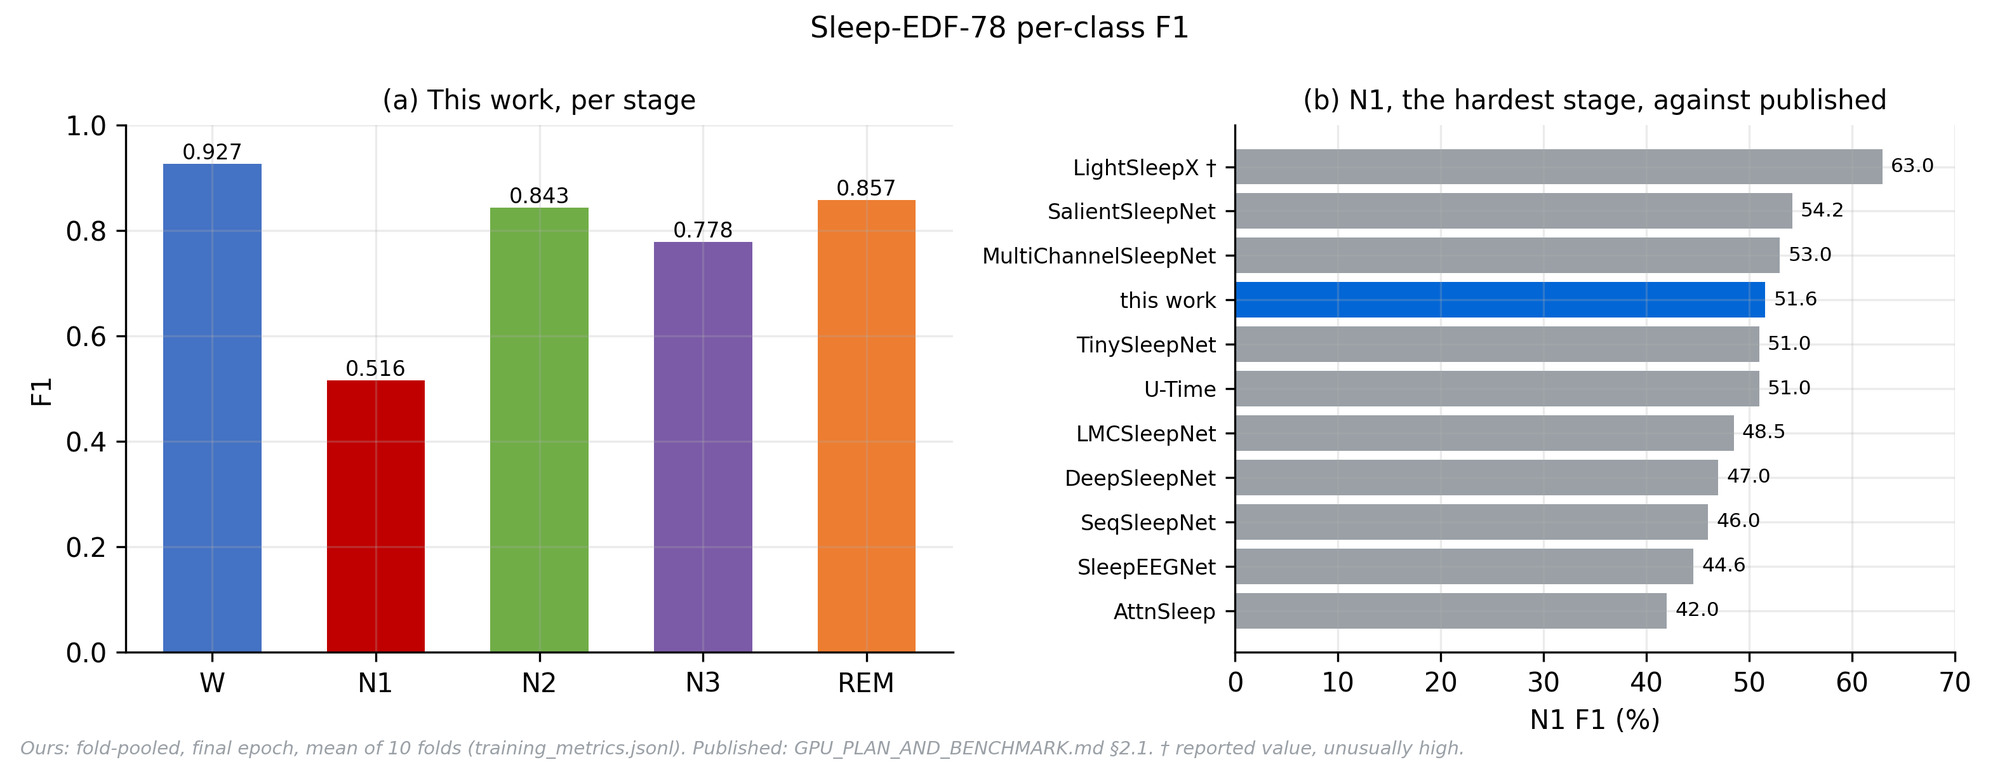
\includegraphics[width=0.85\textwidth]{F19_b1_per_class.jpg}
\caption{B1 per-class F1.}
\label{fig:b1class}
\end{figure}

\subsection{Stage 3 --- Evidence packet (release v2)}

\begin{table}[htbp]
\centering\small
\caption{Calibration and confidence signals of the v2 packet.}
\label{tab:packetres}
\begin{tabularx}{\textwidth}{lY}
\toprule
Signal & Result \\
\midrule
Calibration temperature & 1.0021 (fitted on validation): v2 is already calibrated (EMA, label smoothing) \\
ECE, test & 0.0133 before, 0.0134 after; validation 0.0119 $\rightarrow$ 0.0120 \\
Per-stage reliability (test F1) & W 0.914 high; N2 0.844 high; REM 0.837 high; N3 0.809 high; \textbf{N1 0.507 low} \\
Night confidence vs expert agreement & Test Pearson $r = -0.637$ ($p = 2.0\times10^{-4}$), Spearman $\rho = -0.614$; validation $r = -0.543$ \\
Independent of stage composition & Partial $r = -0.623$ controlling for N1 and REM fraction \\
Tiers (validation-fitted), test mean $\kappa$ & High 0.788 (15 nights) $>$ medium 0.731 (4) $>$ low 0.689 (10): monotone without being fitted on test \\
Triage & Flagging the 10 lowest-confidence nights catches 5 of the 10 worst \\
Derived-metric reliability & 3 robust, 13 fragile, 8 unreliable of 24 (Figure~\ref{fig:reliab}) \\
N1 confidence flag & Threshold 0.475 fitted on validation; not measured on test for v2 \\
\bottomrule
\end{tabularx}
\end{table}

\begin{figure}[htbp]
\centering
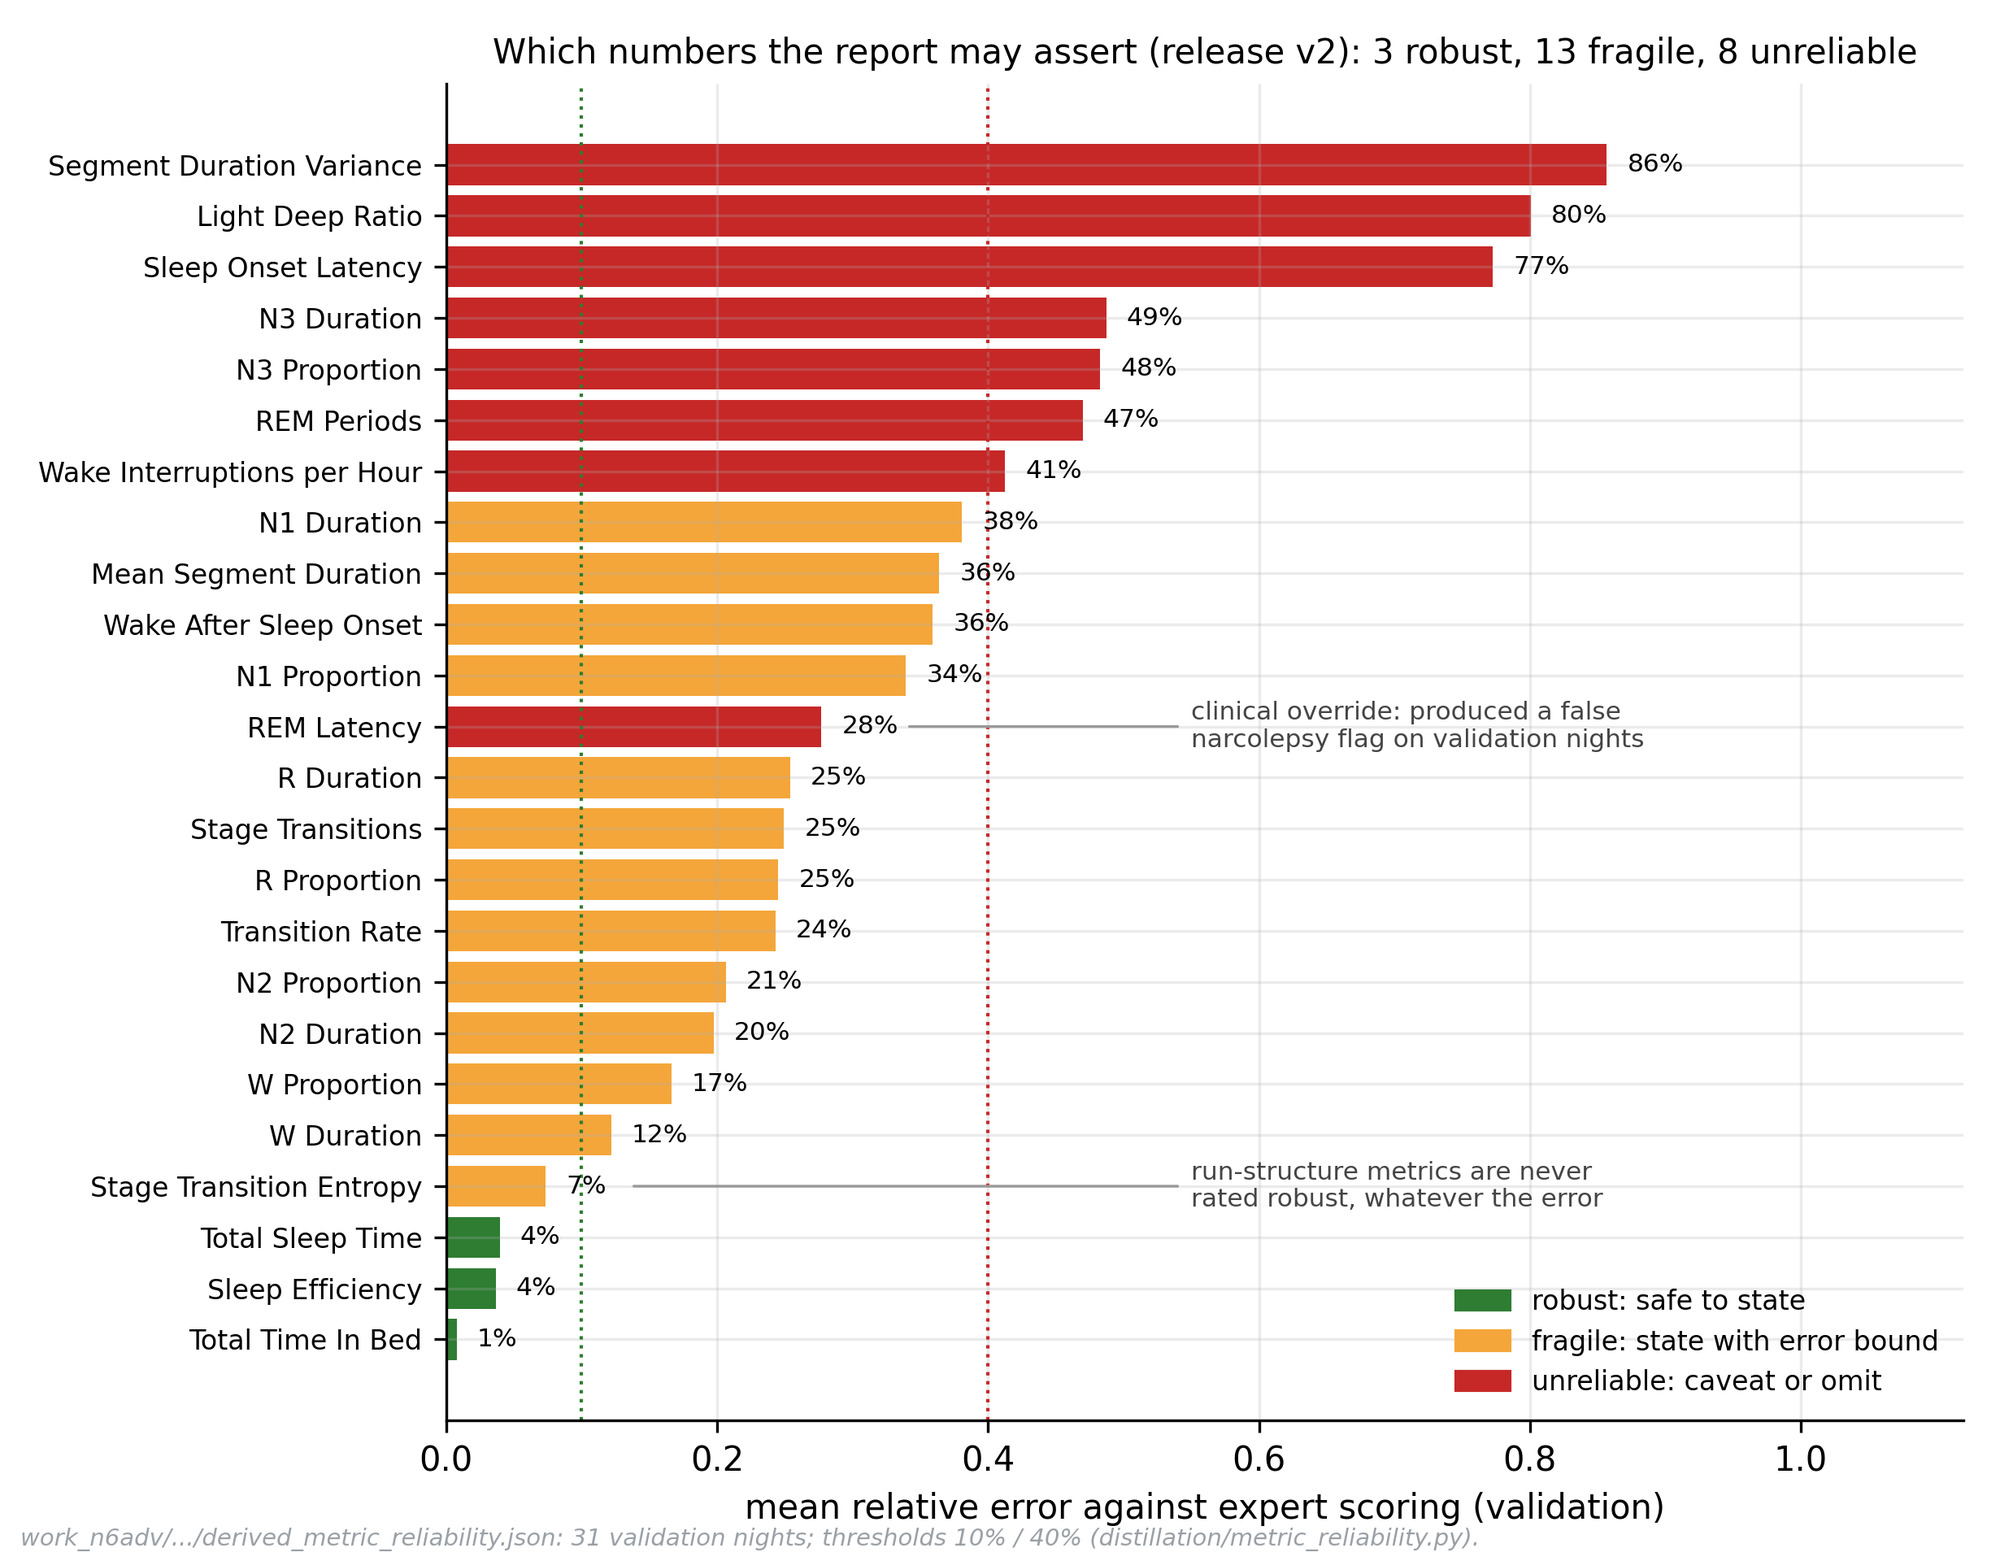
\includegraphics[width=0.85\textwidth]{F30_metric_reliability.jpg}
\caption{Derived-metric reliability: which numbers a report may state.}
\label{fig:reliab}
\end{figure}

\textbf{Plain-language layer.} Clock offsets were reproduced for 168/168 dev and train nights, and the sleep period
used for "awakenings longer than 5 minutes" reproduces each packet's own WASO and sleep-onset latency exactly
(168/168). That awakenings measure turned out to be \emph{unreliable} on v2 (47\% relative error on the 31 dev
nights; within one awakening on 84\% of nights), so it is shown only in the details for a doctor, ungraded. A
second finding: the packet reports stages as a share of the whole recording, while clinical norms use share of
sleep time, so norms are compared only against the latter.

\subsection{Stage 4 --- Small language model}

\textbf{Is the contract achievable?} A large reference model (Gemini 3.1 Flash, temperature 0, structured output +
grammar, prompt P1) produced 30/30 reports at 5/5 with 0 violations and numeric fidelity 1.000 on dev. Its
verifier-passing outputs on the 123 training nights became the training targets.

\textbf{Do untrained small models need training?} With the grammar, the five candidates (Qwen2.5-1.5B,
SmolLM2-1.7B, Gemma-2-2B, Llama-3.2-3B, Phi-3.5-mini) reached 0, 0, 0, 2 and 0 of 31 at 5/5; without it, 0/31 each.
The grammar secures syntax, not meaning; no base model knows the contract.

\begin{table}[htbp]
\centering\small
\caption{Report-model selection (pre-registered bar: $\ge$25/31 at 5/5 on dev).}
\label{tab:slm}
\begin{tabularx}{\textwidth}{lrrrrY}
\toprule
Model & Dev 5/5 & Dev viol. & Test 5/5 & Test viol. & Notes \\
\midrule
Llama-3.2-3B base & 2/31 & -- & -- & -- & Untrained \\
Qwen-Student 1.5B & 10/31 & 0 & 12/29 & 0 & Misses about 1 of 5 items; capacity limit \\
Llama-Student v1 (v1 packets) & 30/31 & 3 & 29/29 & 0 & Fidelity 1.000; peak RAM 4,719 MiB \\
\textbf{Llama-Student v2 (current)} & \textbf{31/31} & \textbf{0} & \textbf{28/29} & 2 (blocked) & Dev fidelity 527/527; test 492/493; \textbf{0 flawed released} \\
\bottomrule
\end{tabularx}
\end{table}

v1 and v2 were scored on different packets and are reported side by side, never pooled (Fisher's exact $p = 1.0$
for the one-night difference). 95\% lower bounds: v1 test $\ge$88.1\%, v2 dev $\ge$88.8\%, \textbf{v2 test
$\ge$82.2\%} (Table~\ref{tab:slm}, Figure~\ref{fig:reports}).

\textbf{The one blocked night (SC4611E0).} REM is 0.12\% of that night, so the packet's sustained-REM latency is
\texttt{None}. The model wrote $-1.0$ instead of omitting the claim. The verifier flagged \texttt{L2.value\_mismatch}
and \texttt{L2.uncited\_quantity}, the text was never rendered, and the agent delivered the fallback summary --- the
system working as designed.

\begin{table}[htbp]
\centering\small
\caption{Verifier ablation on 31 dev nights: reports released with a flaw (definitions pre-registered).}
\label{tab:verabl}
\begin{tabular}{lrrr}
\toprule
Report model & Gate on & Gate off & Gate and grammar off \\
\midrule
\textbf{Llama-Student v2} (v2 packets) & \textbf{0/31} & \textbf{0/31} & \textbf{0/31} \\
Llama-Student v1 (v1 packets) & 0/31 & 1/31 & 2/31 \\
Llama-3.2-3B base (v1 packets) & \textbf{0/31} (all fall back) & 31/31 & 31/31 \\
\bottomrule
\end{tabular}
\end{table}

With the grammar removed, v2's output was byte-identical to its constrained output on all 31 nights: at temperature
0 the grammar never changed a token (Table~\ref{tab:verabl}, Figure~\ref{fig:verabl}). For the fine-tuned model the
verifier is a safety net (it blocked 1 of 29 on test); for an untrained model it is decisive.

\textbf{Determinism.} Llama's chat template wrote today's date into the prompt, so outputs changed from day to day;
pinning the template to the training date fixed it. \texttt{llama-server} did not reproduce the evaluated outputs
(20--23/31 vs 30/31), so the system uses one-shot \texttt{llama-completion}.

\begin{figure}[htbp]
\centering
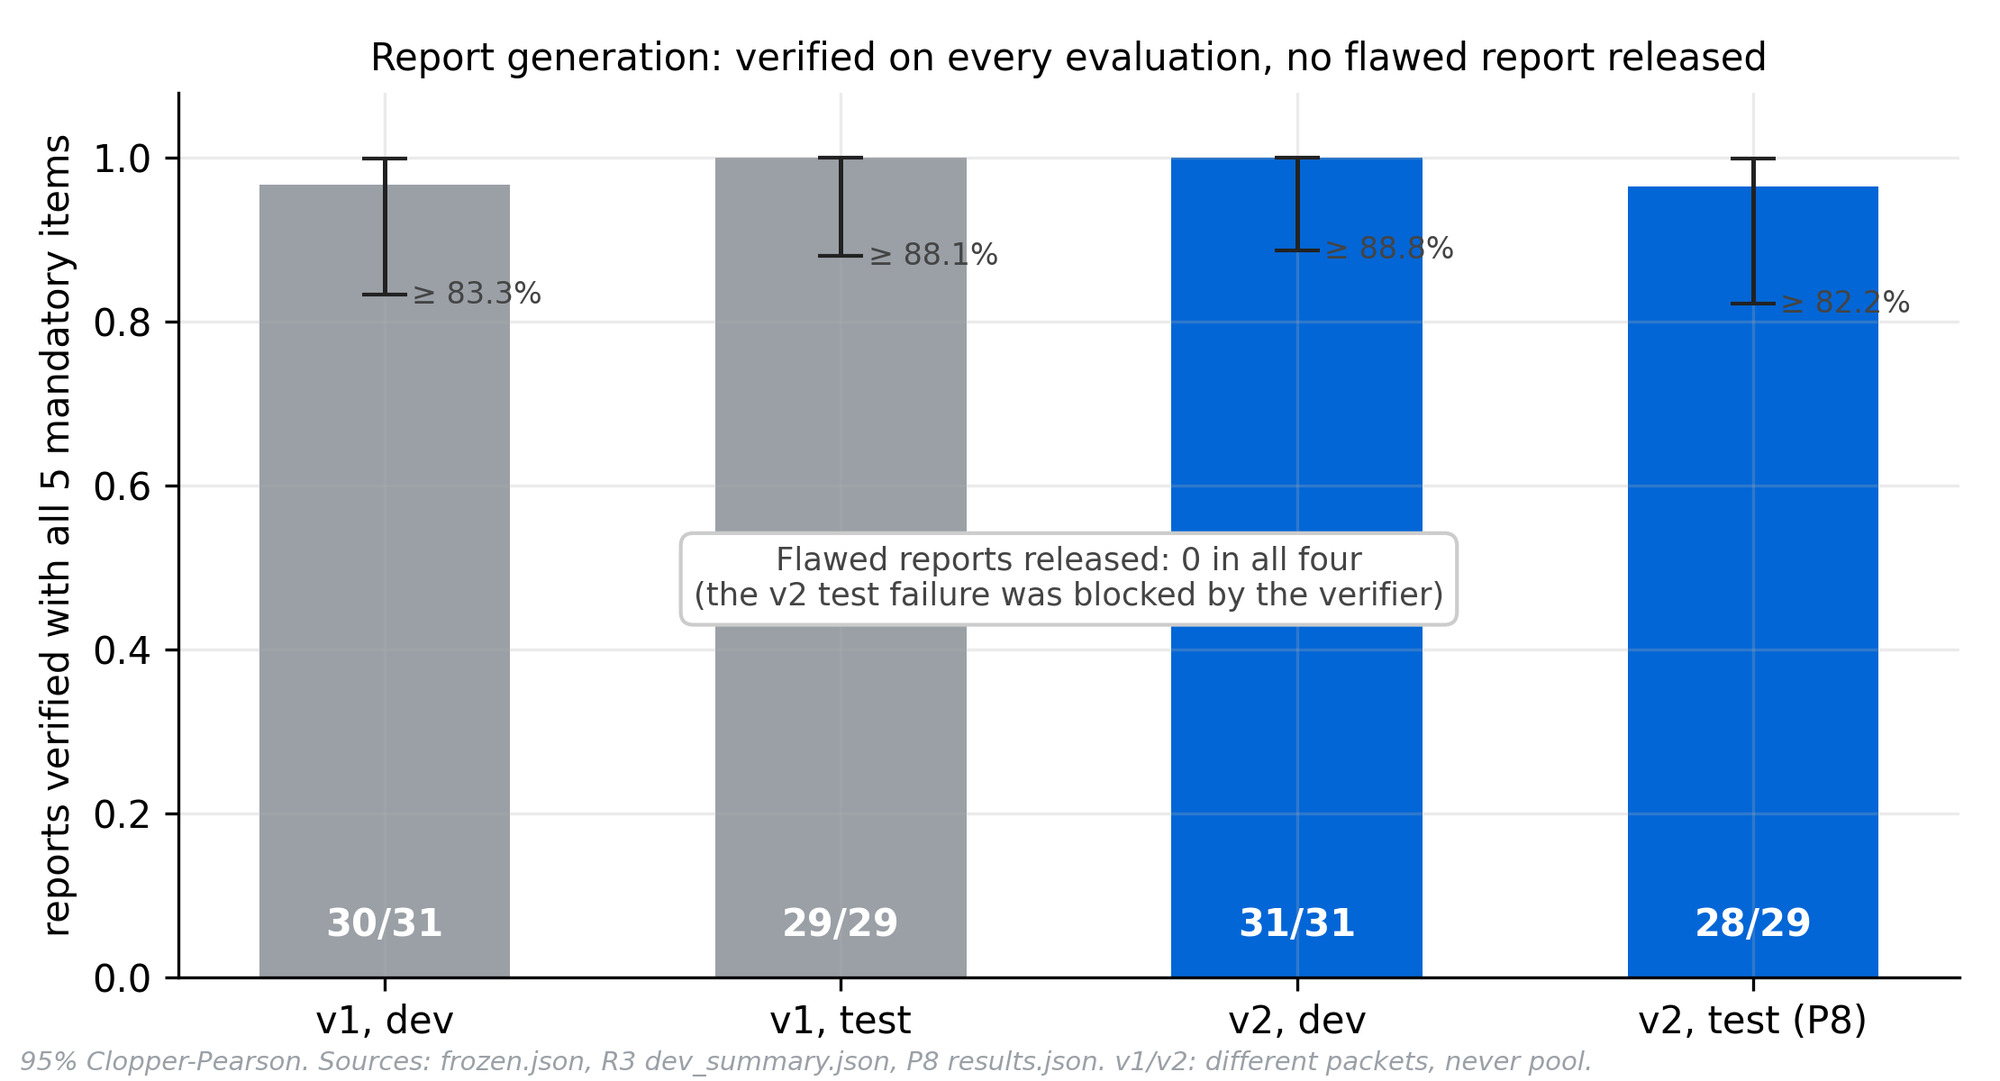
\includegraphics[width=0.85\textwidth]{F25_report_verification.jpg}
\caption{Report verification across releases and splits, with 95\% Clopper--Pearson intervals; 0 flawed reports released in all four.}
\label{fig:reports}
\end{figure}

\begin{figure}[htbp]
\centering
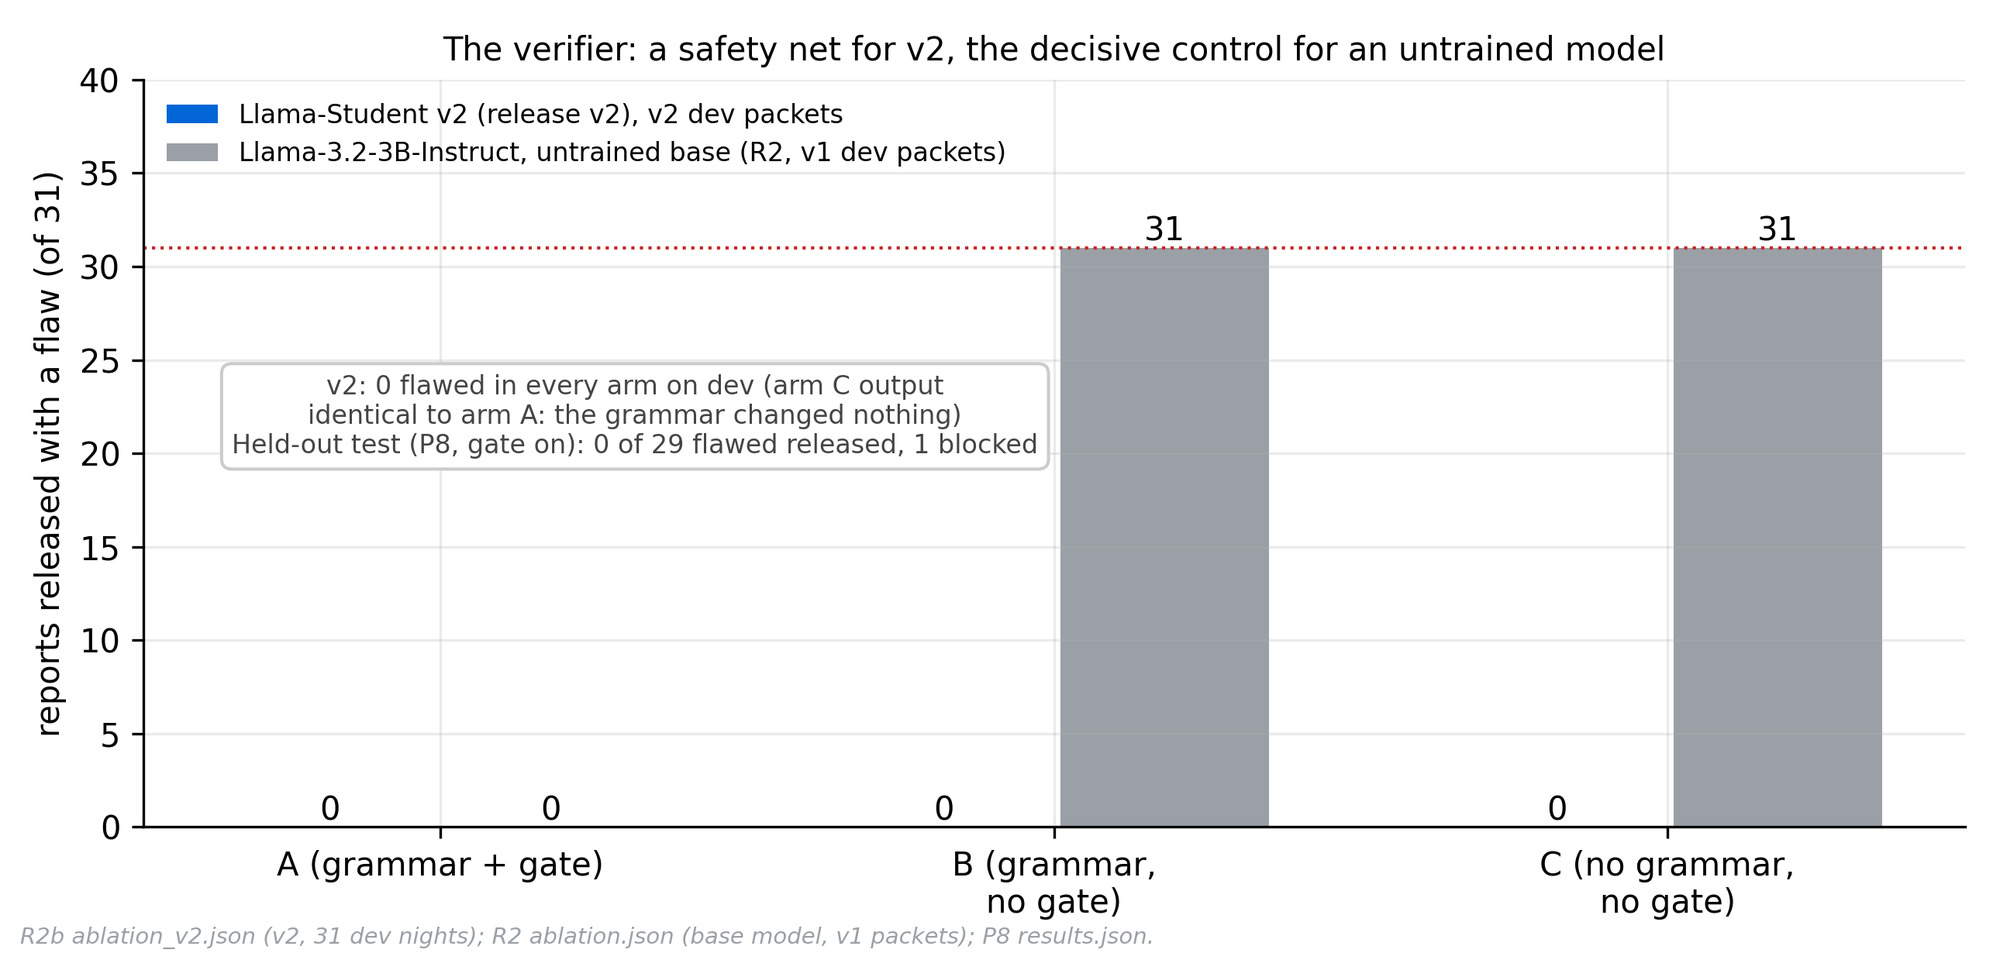
\includegraphics[width=0.85\textwidth]{F20_verifier_ablation.jpg}
\caption{Verifier ablation: flawed reports released with and without the gate.}
\label{fig:verabl}
\end{figure}

\subsection{Stage 5 --- Agentic workflow}

\begin{table}[htbp]
\centering\small
\caption{Fault scenarios (real EDF files from a dev night; injected report-model faults).}
\label{tab:faults}
\begin{tabular}{llll}
\toprule
\# & Scenario & Expected outcome & Result \\
\midrule
S01 & Clean night, no hypnogram & VERIFIED\_REPORT & \yes \\
S02 & Prebuilt packet (Path A) & VERIFIED\_REPORT & \yes \\
S03 & EEG flat for 2\,h & REVIEW\_ONLY Q01 & \yes \\
S04 & EOG missing & VERIFIED\_REPORT & \yes \\
S05 & Fpz-Cz missing, Pz-Oz present & REVIEW\_ONLY W05 & \yes \\
S06 & Recorded at 128\,Hz & VERIFIED\_REPORT (resampled) & \yes \\
S07 & Only 2\,h recorded & REJECTED R03 & \yes \\
S08 & Corrupt header & REJECTED R01 & \yes \\
S09 & Report model crashes once & VERIFIED\_REPORT after retry & \yes \\
S10 & Report model hangs & FALLBACK F02 & \yes \\
S11 & Report model writes invalid claims & FALLBACK F03 & \yes \\
S12 & Device at 82\,$^\circ$C & FALLBACK F01 after 12 waits & \yes \\
S13 & Power cut during generation & VERIFIED\_REPORT, one delivery & \yes \\
S14 & Strong 49\,Hz line noise & VERIFIED\_REPORT at the time & \yes; led to the Q03 check \\
S15 & Two nights of one subject (trend) & -- & deferred (needs history store) \\
\bottomrule
\end{tabular}
\end{table}

\textbf{14/14 pass, 1 deferred} (Table~\ref{tab:faults}). The invariants hold on every run: I1 no unverified text;
I2 every number has provenance; I3 frozen components; I4 no network; I5 expert hypnograms never read by the
workflow; I6 every run ends; I7 every step traced; I8 every failure visible in the review queue. Crash recovery at
eight boundaries produced exactly one delivery each time.

\begin{table}[htbp]
\centering\small
\caption{Further robustness results.}
\label{tab:robust}
\begin{tabularx}{\textwidth}{lY}
\toprule
Check & Result \\
\midrule
Real recordings end to end (Path B, v2, 31 dev nights) & Mean per-night $\kappa$ 0.701 (v1 0.673; v2 higher on 27/31); pooled accuracy 79.5\%, $\kappa$ 0.719; \textbf{30 verified + 1 sent to review (line noise)}; median 78\,s per report on x86 \\
Night boundaries without an expert & Start: median 0, p90 2 epochs; end: median 2, p90 41 epochs (bar 30; accepted deviation) \\
Sampling rates (3 nights $\times$ 2 releases $\times$ 128/256\,Hz) & 18/18 outcomes match 100\,Hz; hypnogram agreement 0.992--1.000 \\
Line noise & A 49\,Hz tone at 1$\times$ EEG RMS drops $\kappa$ 0.775 $\rightarrow$ 0.340, and the verifier cannot see it, so an input check (Q03/W10) was added \\
Quality flags predict worse staging & Dev nights flagged W02: $\Delta\kappa$ $-0.138$, 95\% CI [$-0.202$, $-0.072$] \\
Reproducibility (real model, 2 runs $\times$ 31 nights) & 31/31 byte-identical report pages \\
Preprocessing parity with training & 31/31 exact (EEG, 34 features, probabilities) \\
\bottomrule
\end{tabularx}
\end{table}

\begin{figure}[htbp]
\centering
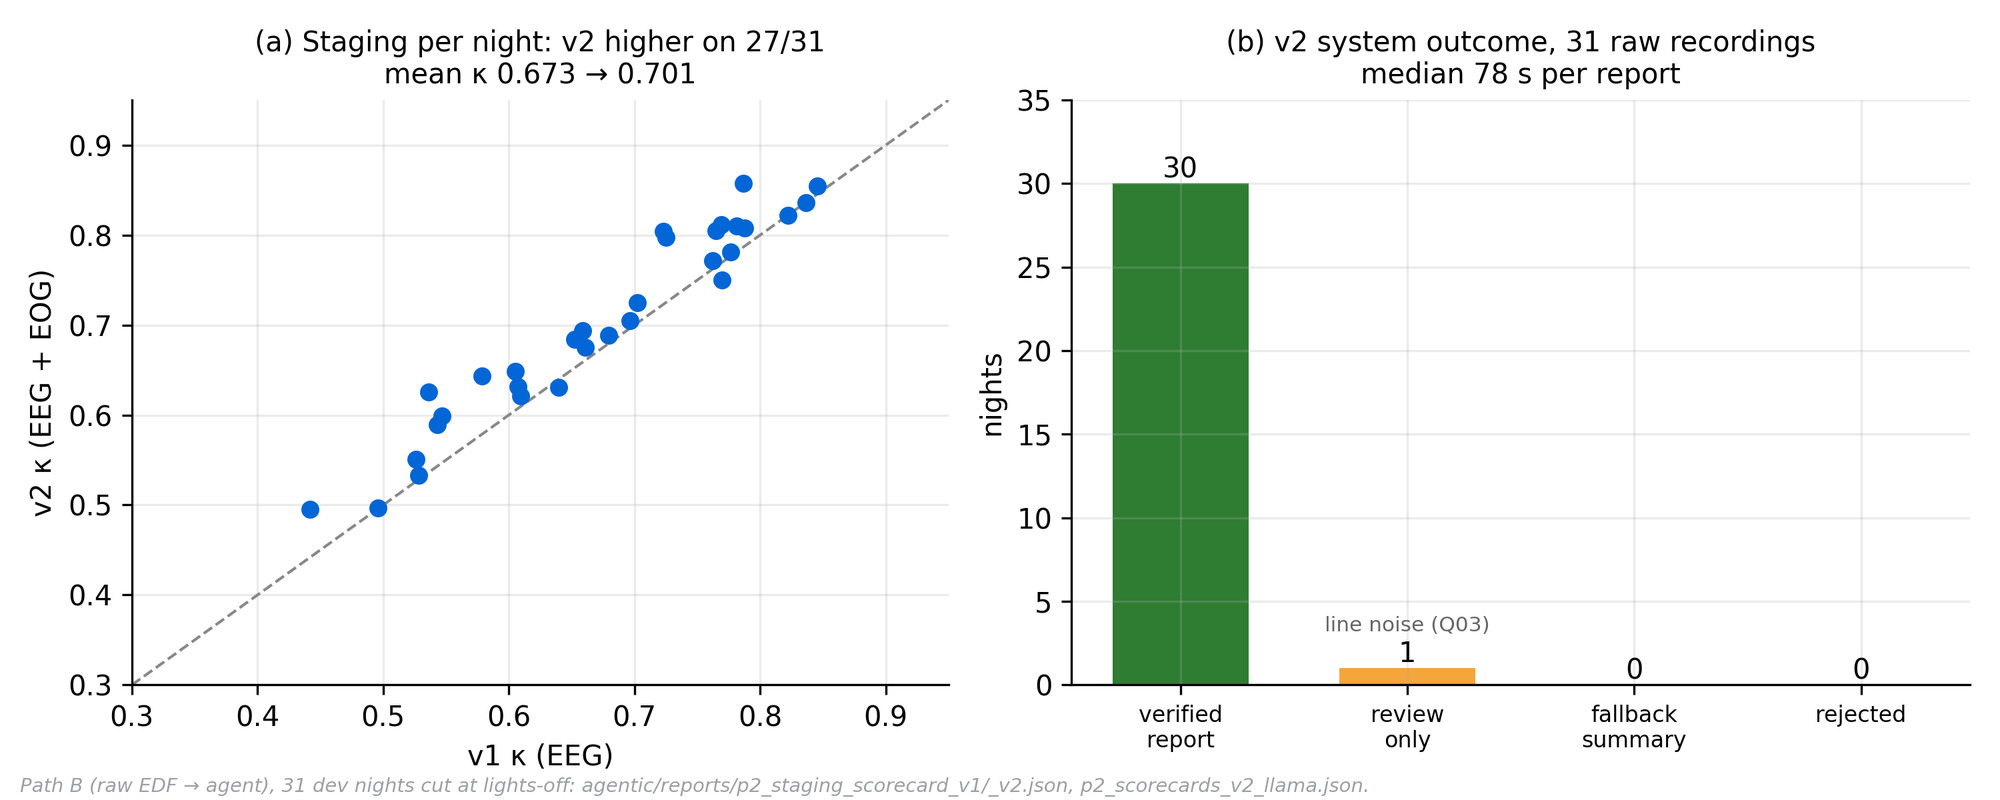
\includegraphics[width=0.85\textwidth]{F29_real_recordings.jpg}
\caption{Real recordings end to end (Path B): v2 against v1 per night.}
\label{fig:pathb}
\end{figure}

\begin{figure}[htbp]
\centering
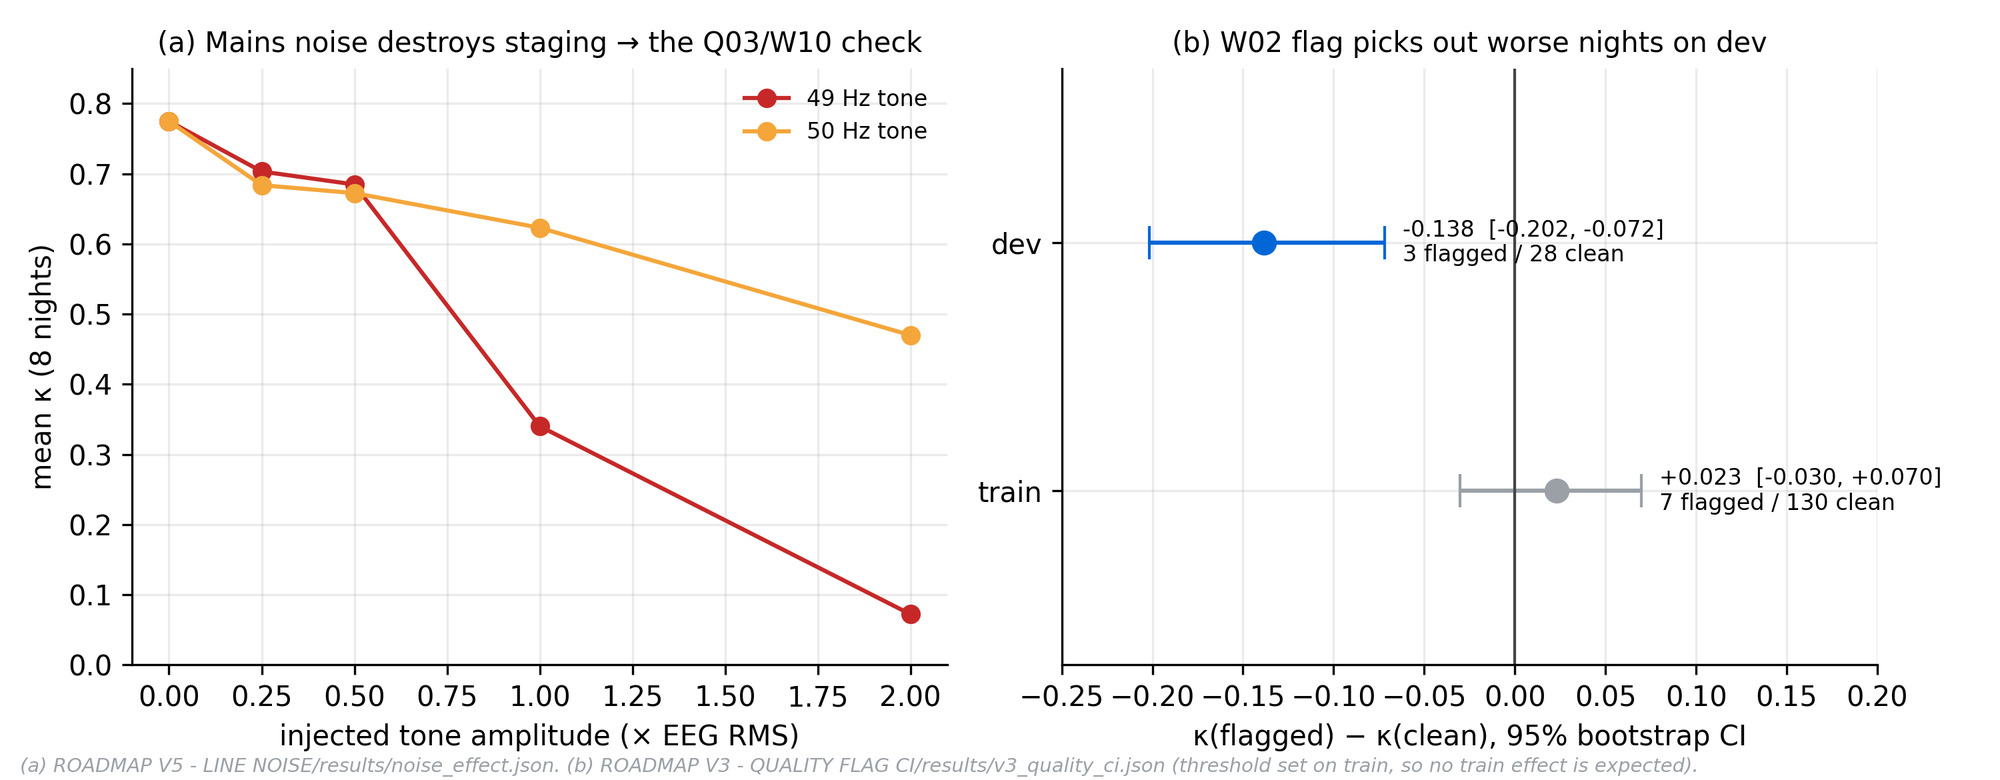
\includegraphics[width=0.85\textwidth]{F31_quality_checks.jpg}
\caption{Signal-quality checks and the effect of line noise.}
\label{fig:quality}
\end{figure}

\begin{figure}[htbp]
\centering
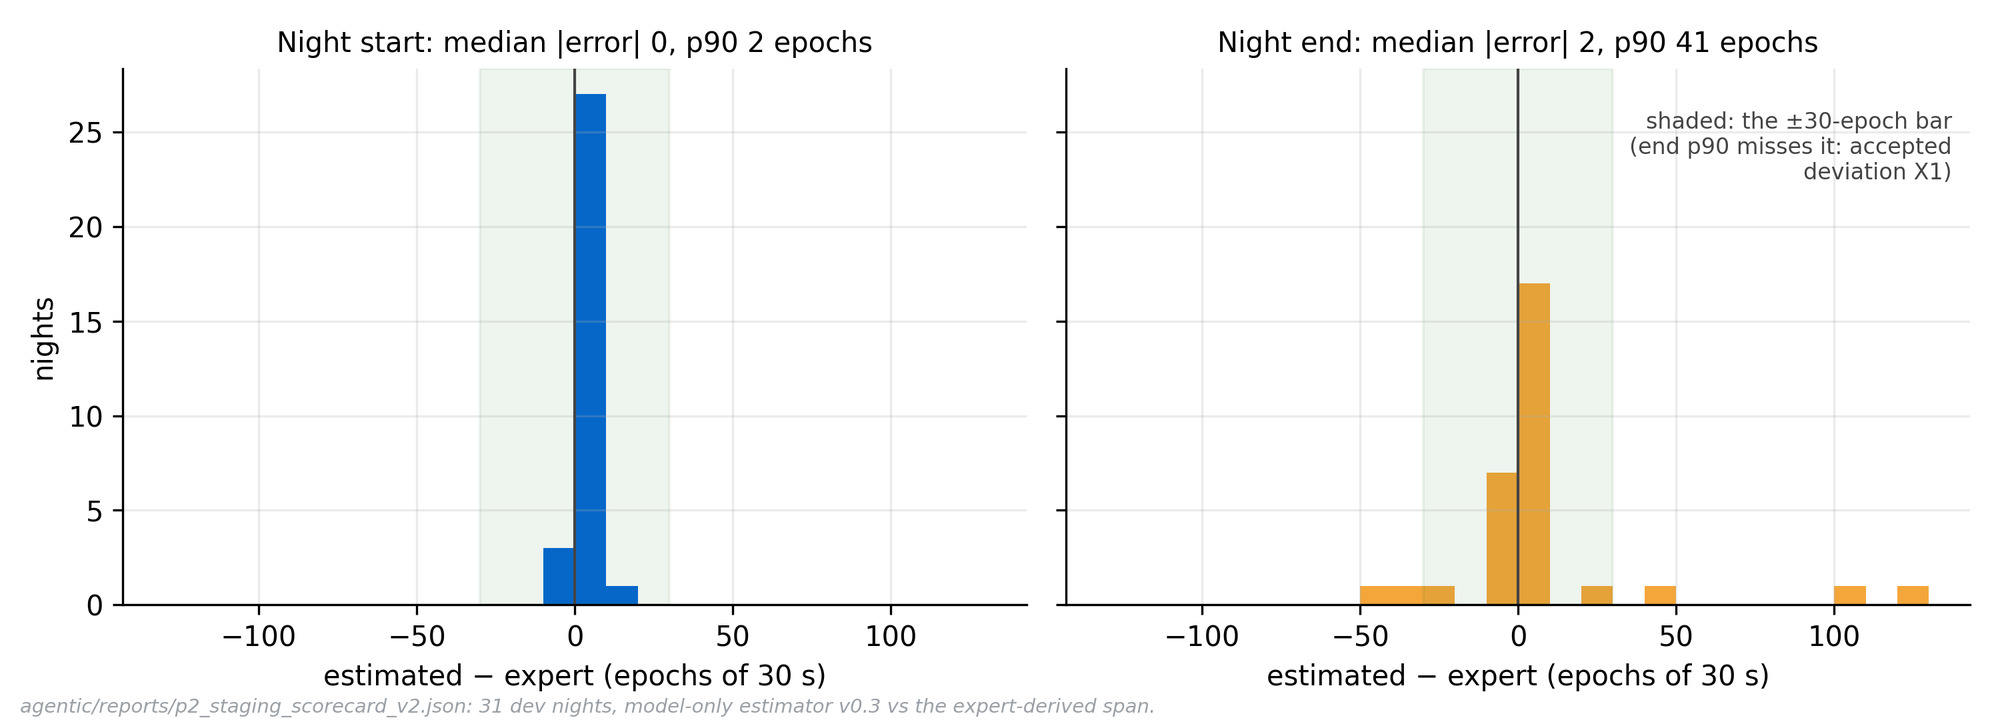
\includegraphics[width=0.85\textwidth]{F32_night_boundaries.jpg}
\caption{Night boundaries found without an expert.}
\label{fig:bounds}
\end{figure}

\subsection{Stage 6 --- Edge-device simulation (Raspberry Pi 5, 16\,GB)}

\textbf{L1 and L2: offline containers limited like the Pi.} The agent ran unchanged in a Linux x86-64 Docker container
(4 CPUs, 16\,GiB, \texttt{--network none}, project and data read-only, llama.cpp b10927 compiled inside the image) on a
second Windows PC (Table~\ref{tab:l1}). The cgroup limits were confirmed from inside the container. The first run of
this experiment exposed three faults in the container bundle (missing llama.cpp shared libraries, a missing module and a
zip step); they were fixed and the experiment repeated, and only the repeated run is reported. In it:
\begin{itemize}
  \item Staging on all 31 raw dev recordings matched the Windows reference run exactly at the hypnogram level, with
  probability differences more than five times below the acceptance bar.
  \item The report model, run on all 31 evidence packets, produced 31/31 verified reports whose text was
  \textbf{byte-identical} to the reference PC's, at a median of 151\,s per report and a peak of 5.16\,GB for the whole
  process tree. The three-night end-to-end run (raw EDF to delivered page) reproduced the reference outcome on all three;
  the night the reference run sent to review (SC4111E0, line noise, Q03) was sent to review again.
  \item Under ARM64 emulation (QEMU), the staging stage on 8 nights gave identical hypnograms with a maximum probability
  difference of $7.7\times10^{-7}$. The emulated run was seven times slower (133\,s against 18\,s per night), which
  is a property of the emulation and not a timing of the Pi.
\end{itemize}
These are x86 timings on a desktop CPU; they bound nothing about the Pi's speed. They do show that the whole release
runs, offline and verified, inside the memory the Pi has, and that its output does not depend on the operating system or
compiler.

\begin{table}[htbp]
\centering\small
\caption{Edge simulation in Docker (4 CPUs / 16\,GiB / no network): x86-64 and ARM64 under emulation.}
\label{tab:l1}
\begin{tabularx}{\textwidth}{lYl}
\toprule
Check & Result & Verdict \\
\midrule
P1 no network & TCP to 1.1.1.1:53 and DNS lookup both blocked & \textbf{met} \\
P4 no secrets in the image & No \texttt{.env}, no API-key pattern in the mounted project or the image & \textbf{met} \\
Release pins & All pinned hashes match inside the container; \texttt{llama-completion} starts & \textbf{met} \\
Staging parity, Linux x86 vs reference PC & 31/31 nights, 61/61 arrays (pass 1 + pass 2) with identical hypnograms; max $|\Delta p| = 1.8\times10^{-5}$ (bar $10^{-4}$) & \textbf{met} \\
Report model, 31 dev packets (Path A) & 31/31 VERIFIED\_REPORT; text identical to the reference on 31/31; median 151\,s, p95 160\,s; peak 5.16\,GB & \textbf{met} \\
End to end, 3 raw nights (Path B) & Outcome equals the reference on 3/3 (2 verified, SC4111E0 review Q03); staging max $|\Delta p| = 8.3\times10^{-7}$; median 158\,s; peak 5.64\,GB & \textbf{met} \\
E1 staging parity on ARM64 (QEMU), 8 SC nights & 15/15 arrays with identical hypnograms; max $|\Delta p| = 7.7\times10^{-7}$ & \textbf{met in emulation} \\
Not yet run & ARM report model; ST nights on ARM; Raspberry Pi 5 timing, heat and power; 7-night soak & open \\
\bottomrule
\end{tabularx}
\end{table}

\begin{table}[htbp]
\centering\small
\caption{Per-night budget on the Raspberry Pi 5 (analytical estimates, not measurements).}
\label{tab:budget}
\begin{tabular}{lr}
\toprule
Step & Estimate \\
\midrule
Ingest + quality checks & 5--20\,s \\
Study period (two-pass staging) & 5--15\,s \\
Preprocess (resample, epochs, 34 features) & 10--40\,s \\
Staging (175\,K params, CPU) & 2--10\,s \\
Packet & $<$5\,s \\
Report prefill ($\sim$1,100 tokens at an assumed 15--30 tokens/s) & 40--80\,s \\
Report generation ($\sim$1,200 tokens at 3.06--4.37 tokens/s; ceiling 7.43) & 266--380\,s \\
Verifier + render & $<$2\,s \\
\midrule
\textbf{Total per night} & \textbf{$\approx$6--9 min} (x86 measured: median 78\,s per report native, 151\,s in the 4-CPU container) \\
\textbf{Peak memory} & \textbf{$\approx$6--8\,GB} of 16\,GB (measured in the x86 container: 5.2\,GB report, 5.6\,GB end to end) \\
\bottomrule
\end{tabular}
\end{table}

Memory bandwidth, not memory size, sets the speed (Table~\ref{tab:budget}): the 16\,GB board is not faster than the
8\,GB one, but it keeps every model resident with the full context. \textbf{Pre-registered acceptance bars for the
Pi:} staging parity max $|\Delta p| \le 10^{-4}$ with identical hypnograms (E1); dev 5/5 not below the x86 result,
with every failure caught by the verifier; P95 $\le$15 min per night; peak $\le$10\,GB; no thermal throttling with
the Active Cooler at 25\,$^\circ$C; all fault scenarios and a 7-night unattended soak with 0 crashes. In the container the
parity, report-parity and peak-memory bars are met; the time, heat and soak bars need the device.

\section{ Analysis of Results}

\begin{itemize}
  \item \textbf{Measurement before modelling.} The largest single change in the project came from evaluation, not
  architecture: subject leakage inflated $\kappa$ by about 0.16, and misaligned labels cost about 3 accuracy points.
  Every later result depends on fixing both.
  \item \textbf{Distillation works only with a better teacher.} The negative KD result has a mechanism, and the fix
  (an ensemble of comparable, diverse students) followed from it. Distillation's lasting benefit was calibration,
  which the packet then turns into usable confidence.
  \item \textbf{EOG helps where expected.} Like for like, EOG adds +0.018 $\kappa$, with the gains on N1 and REM,
  the stages defined partly by eye movements; without EOG the model still beats v1.
  \item \textbf{Trust signals are real.} Night confidence ranks nights by agreement with the expert on test without
  being fitted there, and it is not a proxy for stage composition.
  \item \textbf{Training, not the grammar, made the report model correct.} The grammar fixes syntax; fine-tuning
  supplied the semantics; the verifier is the safety net that caught the one remaining error on test.
  \item \textbf{The agent turns failure into a truthful outcome.} Every fault produced a defined page; no scenario
  produced a wrong report.
  \item \textbf{The system is portable.} Moved to Linux, in a container with no network and Pi-like limits, the
  staging stage produced the same hypnograms on every night, and the report model reproduced the reference text
  byte for byte on all 31 packets. The same staging code gave identical hypnograms when run for ARM64 under emulation.
\end{itemize}

\section{Observations:}

\begin{itemize}
  \item \textbf{N1 remains the weak stage} (F1 0.51 on test). Expert agreement on N1 is itself only 25--45\%, so the
  packet marks N1 low-reliability rather than claiming more.
  \item \textbf{Rare-stage nights stress the report model.} The one test failure was a night with almost no REM,
  where the correct behaviour was to omit a claim.
  \item \textbf{The verifier checks claims against the packet, not the packet against the signal.} Line noise
  produced a confident, wrong packet that the verifier could not see; only input quality control protects against it.
  \item \textbf{Small sets limit resolution.} With 15 test subjects the CI on $\kappa$ is about $\pm$0.05; several
  later changes returned statistical ties because the evaluation could not resolve them.
  \item \textbf{Statistical significance.} v2 vs v1 staging: Wilcoxon $p = 0.0009$, $\Delta\kappa$ CI excludes 0;
  the EOG ablation CI excludes 0, better on 5/5 folds; the quality-flag effect CI excludes 0 on dev; the
  night-confidence correlation has $p = 2.0\times10^{-4}$ on test.
\end{itemize}

\section{ Comparative Analysis}\label{sec:comparative}

The comparison is made at three levels: staging accuracy against published models and an offline tool, report
generation against untrained models and LLM reporting systems, and the system as a whole against the best existing
work on every aspect (Tables~\ref{tab:compare} and~\ref{tab:scorecard}).

\begin{figure}[htbp]
\centering
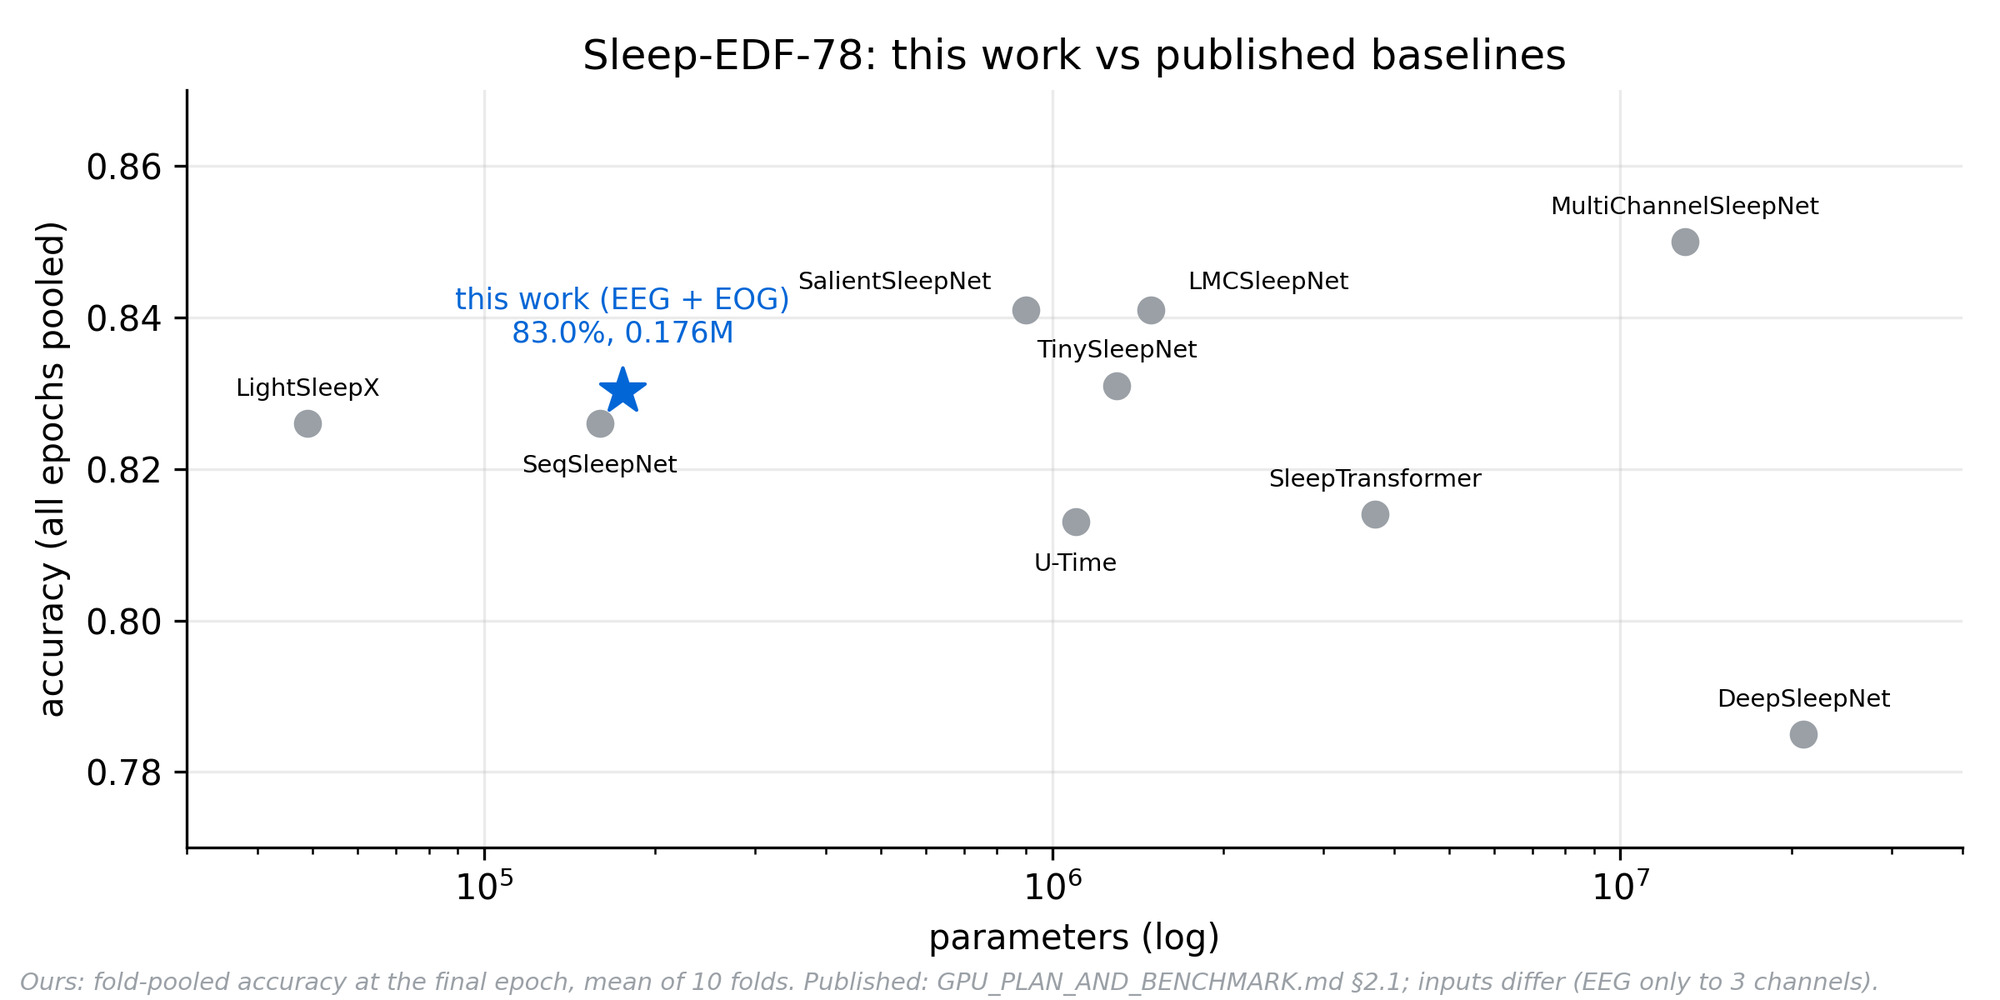
\includegraphics[width=0.85\textwidth]{F18_b1_vs_published.jpg}
\caption{B1 against published models on Sleep-EDF-78 (ours pooled like the papers, final epoch).}
\label{fig:b1pub}
\end{figure}

\begin{figure}[htbp]
\centering
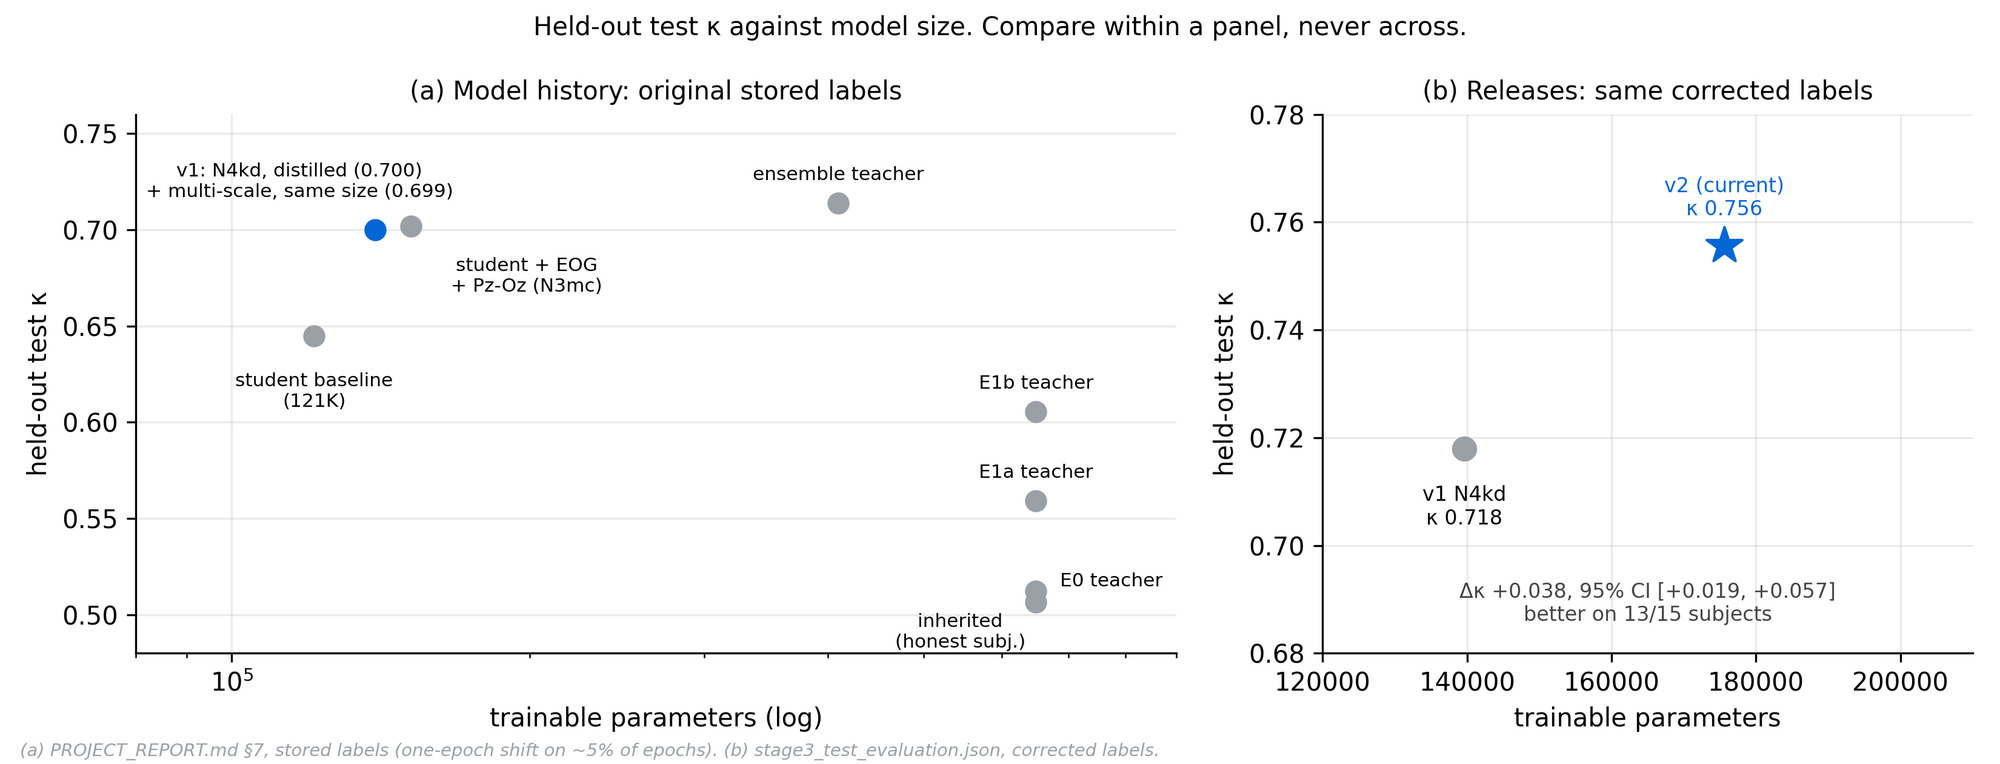
\includegraphics[width=0.85\textwidth]{F14_params_vs_kappa.jpg}
\caption{Model size against $\kappa$; v1 against v2 on the same corrected labels.}
\label{fig:size}
\end{figure}

\begin{figure}[htbp]
\centering
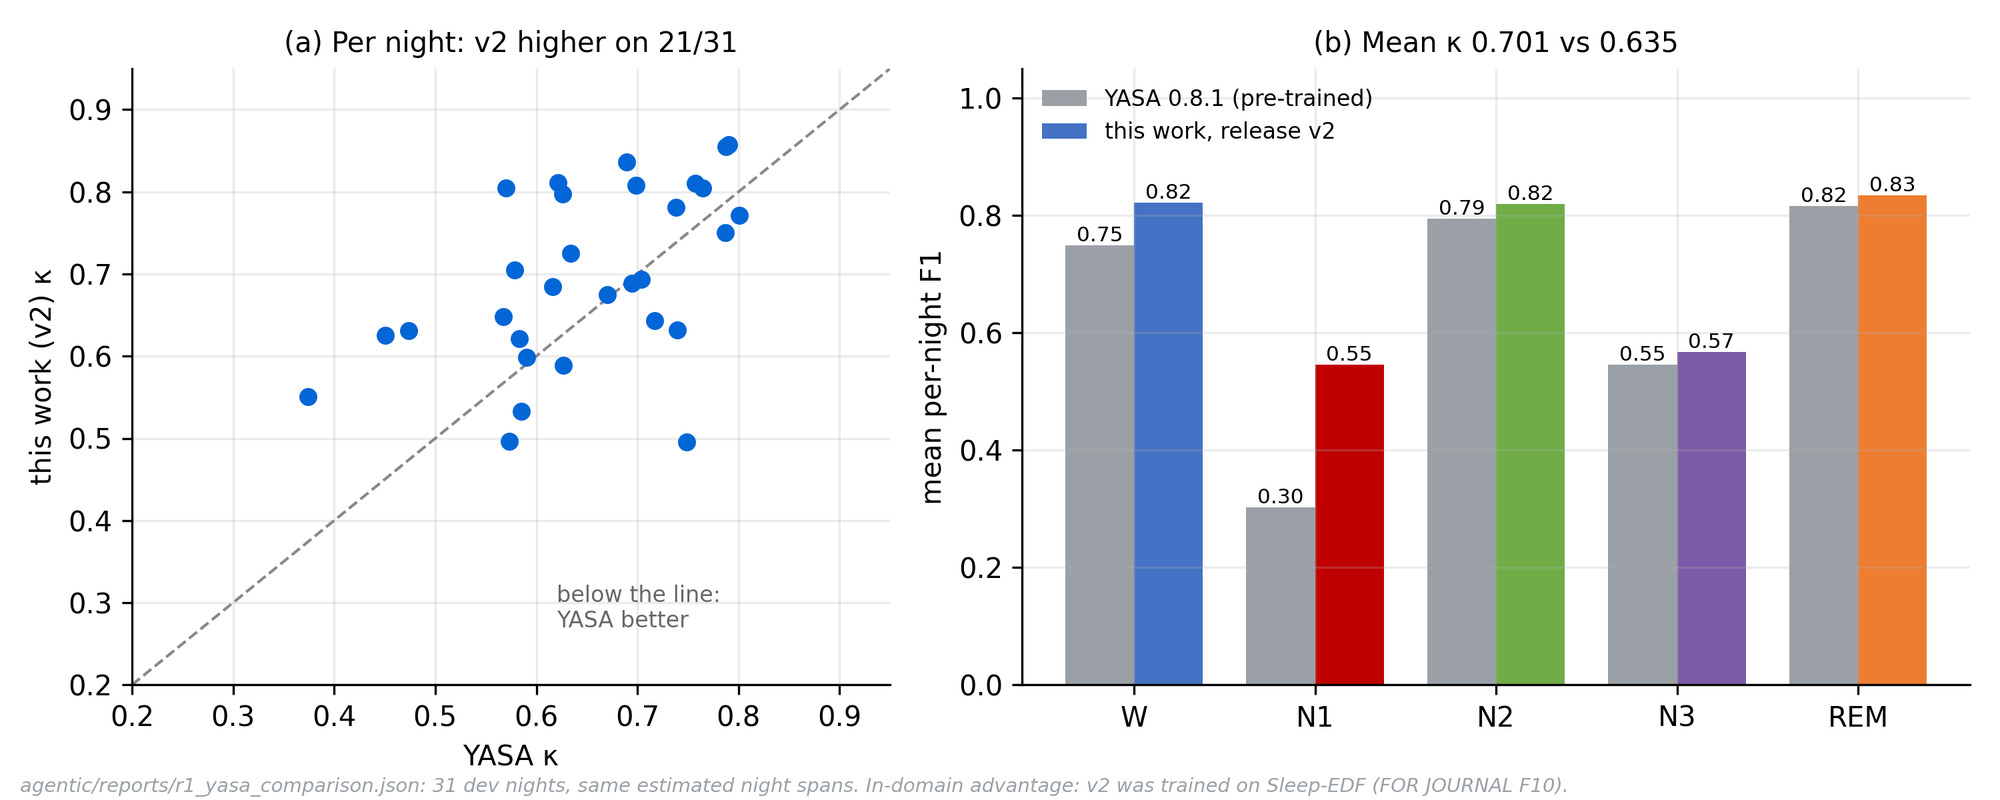
\includegraphics[width=0.85\textwidth]{F28_vs_yasa.jpg}
\caption{Same-night comparison with YASA on the 31 dev nights.}
\label{fig:yasa}
\end{figure}

\begin{table}[htbp]
\centering\small
\caption{Comparative analysis.}
\label{tab:compare}
\begin{tabularx}{\textwidth}{p{0.24\textwidth}Y}
\toprule
Comparison & Result \\
\midrule
Staging vs published (B1, Table~\ref{tab:published}) & $\kappa$ 0.769--0.775, level with TinySleepNet, LightSleepX and LMCSleepNet (0.77), below SleepSatelightFTC (0.787) and MultiChannelSleepNet (0.79); macro-F1 78.4--79.0 above TinySleepNet and LMCSleepNet; \textbf{175,599 parameters, 5--74$\times$ smaller} than the models at our level except LightSleepX (Figures~\ref{fig:b1pub}, \ref{fig:size}) \\
Per class (B1) & Strongest on N1 (51.6--53.1) and REM (85.7--85.9); weaker on N2 ($\sim$2 points below the best) and N3 ($\sim$3.5 points below) \\
Fair EEG-only comparison & \texttt{full\_eeg} CV $\kappa$ 0.765; test with EOG removed 0.744 \\
Same nights vs YASA 0.8.1 (31 dev nights) & Accuracy 0.790 vs 0.744; $\kappa$ 0.701 vs 0.635; macro-F1 0.717 vs 0.642; N1 F1 0.545 vs 0.302; better on 21/31 nights. Our model is in-domain; YASA is not (Figure~\ref{fig:yasa}) \\
vs our teacher & v2 beats ENSmc on every metric with 43\% of its parameters (combined effect of labels, EOG and recipe) \\
vs untrained SLM & Base Llama-3.2-3B: 2/31 at 5/5, and 31/31 flawed without the gate; v2 student: 31/31 dev, 28/29 test, 0 flawed released \\
vs LLM reporting systems (Table~\ref{tab:llm}) & Others check output after generation by humans or LLMs; ours blocks a report \textbf{before release} with a deterministic check, runs offline at temperature 0, and reruns byte-identically \\
Size & Staging model 0.70\,MB; the report model (2.02\,GB) is 99.9\% of the system footprint \\
\bottomrule
\end{tabularx}
\end{table}

\begin{table}[htbp]
\centering\scriptsize
\caption{Head-to-head scorecard against the best existing work. "Ours" figures are measured in this project (release v2 unless stated); verdicts are qualified where protocols differ.}
\label{tab:scorecard}
\begin{tabularx}{\textwidth}{p{0.17\textwidth}YYp{0.14\textwidth}}
\toprule
Aspect & Best existing (who, figure) & Ours & Verdict \\
\midrule
Automatic check of generated text & Human review or LLM-as-judge, after generation & Deterministic verifier before release; 0 flawed reports released on test (28/29 verified, 1 blocked) & \textbf{Ahead} \\
Complete report from a local model & Local LLMs on OSA: "needs significant improvement" (different task) & 31/31 dev and 28/29 test at 5/5; base model 2/31 & \textbf{Ahead} \\
Effect of the gate & No published ablation & Untrained model: 31/31 flawed without the gate, 0/31 with it & \textbf{Ahead} \\
Uncertainty in the report & Reported (SleepTransformer, YASA), not enforced in text & Hedging enforced by the verifier from measured error & \textbf{Ahead} \\
Offline and private & Local-LLM study (Seifen et al.) & Fully offline on CPU; network verified off in a container; 31/31 reports verified and identical there & \textbf{Ahead} \\
Reproducibility & Not reported & 31/31 byte-identical reruns; cross-platform staging parity 31/31 & \textbf{Ahead} \\
Student vs teacher & KD students usually approach the teacher & $\kappa$ 0.756 vs 0.732 on held-out test (confound disclosed) & \textbf{Ahead} (qualified) \\
Size for the accuracy & LightSleepX: 49\,K, $\kappa$ 0.77 & 176\,K, $\kappa$ 0.769--0.775 (B1) & Level \\
N1 F1 & SalientSleepNet 54.2 & 51.6--53.1 (B1) & Level \\
REM F1 & SalientSleepNet 85.8 & 85.7--85.9 (B1) & Level \\
Overall staging & MultiChannelSleepNet: 85.0\%, $\kappa$ 0.79, 13\,M & 83.0--83.5\%, $\kappa$ 0.769--0.775, 0.176\,M & Behind by $\sim$1.5 points, 74$\times$ smaller \\
N3 F1 & MultiChannelSleepNet 81.8 & 77.8--78.3 (B1) & Behind \\
External validation & SleepVLM (external cohort); SleepFM (SHHS) & None yet & Behind \\
Training data & SleepFM: $\sim$65,000 people & 85 subjects & Behind (by design) \\
Clinician evaluation & Seifen et al.; guidance-SLM human evaluation & None yet & Behind \\
Clinical scope & Products: apnea, arousals, leg movements & Staging and architecture only & Behind (out of scope) \\
Regulatory clearance & FDA 510(k), AASM certification & None & Behind (out of scope) \\
Edge hardware & Dreem 3S headband; Micro SleepNet on a phone & x86 container (4 CPUs / 16\,GB, offline) measured end to end; ARM64 staging parity in emulation; no Pi timing yet & Behind (planned) \\
\bottomrule
\end{tabularx}
\end{table}

\textbf{Summary: ahead on 7, level on 3, behind on 8.} The work leads on everything that makes a \emph{generated
report trustworthy}, matches the field on model size and the hard stages, and is behind on the evidence a clinic
would expect --- external validation, clinician rating, clinical scope and measured hardware --- which is exactly
the Phase~II plan in Chapter~5. The comparison with published staging models is indicative rather than exact:
their numbers are as published, on their own preprocessing and labels, whereas ours use corrected labels.

\chapter{Conclusion and Scope for further Research}
This project built and evaluated, end to end, an offline system that turns one night of EEG + EOG into a written
sleep report whose every claim is checked before release. In the order the work was done:

\begin{enumerate}
  \item \textbf{Knowledge distillation} worked only after the evaluation was made honest and the teacher was made
  genuinely better than the student; an ensemble of diverse compact students provided that teacher, and
  distillation's clearest gain was calibration.
  \item \textbf{The staging student} (release v2, 175,599 parameters, EEG + EOG) reaches $\kappa$ 0.756 on held-out
  subjects and $\kappa$ 0.769--0.775 on the standard Sleep-EDF-78 protocol, competitive with models 5--74$\times$
  larger, and degrades gracefully without the eye channel.
  \item \textbf{The evidence packet} turns predictions into a contract that carries measured trust: per-stage
  reliability, a night-confidence tier that predicts expert agreement without ground truth, and the measured
  reliability of each of 24 derived metrics.
  \item \textbf{The fine-tuned SLM}, behind a frozen deterministic verifier, released 28/29 verified reports and
  \textbf{no flawed report} on the locked test set; the one flawed generation was blocked.
  \item \textbf{The agentic workflow} delivered the correct, truthful outcome in every fault scenario tested, with
  eight safety invariants holding and byte-identical reruns.
  \item \textbf{The edge design} fits a Raspberry Pi 5 on paper (about 6--9 minutes and 6--8\,GB per night), and the
  first simulation levels hold: in an offline container with Pi-like limits (4 CPUs, 16\,GB), the network was off, no
  secrets were visible, staging matched the reference on 31/31 nights, and the report model produced 31/31 verified
  reports with text identical to the reference, at 151\,s and 5.2\,GB peak per report; staging gave identical hypnograms
  under ARM64 emulation on 8 nights.
\end{enumerate}

The safe summary claim is: \emph{a 0.18\,M-parameter staging model competitive with far larger models, joined to a
local 3\,B report model whose output is released only after a deterministic check, with no flawed report released
on held-out data.} "Verified" here means consistent with the packet; clinical usefulness is not yet shown.

\section*{Scope for further research (Phase II), in priority order}

\begin{enumerate}
  \item \textbf{Edge measurements:} extend the ARM64 check to Sleep Telemetry nights and to the report model, build the
  overnight replay scheduler and the history store needed for multi-night trends (scenario S15), then measure latency,
  temperature and power on a Raspberry Pi 5 with a 7-night soak, and freeze an edge release with one logged
  evaluation.
  \item \textbf{External validation} on MESA and CFS, which buys both statistical power and clinical credibility.
  \item \textbf{A blinded clinician rating} of reports (even 2--3 raters on 20 reports), and a reader study of the
  plain-language summary with non-experts.
  \item \textbf{Benchmark hygiene:} re-run B1 with an inner early-stopping split and a pooled confusion matrix;
  retrain the teacher on corrected labels or drop the "beats its teacher" claim; check every published row against
  its original paper.
  \item \textbf{Multi-scorer soft labels} (e.g.\ DOD-H/DOD-O, five scorers per epoch), so distillation targets
  reflect real inter-scorer uncertainty rather than model disagreement.
  \item \textbf{A smaller report model} (1--1.5\,B) trained to the 5/5 bar, roughly halving edge latency;
  speculative decoding and prompt-prefix caching as lower-risk speed-ups.
  \item \textbf{A new locked evaluation set}, since the current test set has been used for v2 and cannot evaluate
  a later model.
\end{enumerate}

\appendix
\chapter{Code, Configuration and Reproduction}
\section{Repository layout}

\begin{table}[htbp]
\centering\small
\caption{Key paths in the project repository.}
\begin{tabularx}{\textwidth}{p{0.36\textwidth}Y}
\toprule
Path & Contents \\
\midrule
\texttt{distillation/} & Splits, teacher and student trainers, KD loss, ensemble, calibration, decoder, night confidence, metric reliability, N1 flag, packet builder (v1) \\
\texttt{ADDING EOG VERSION - *} & EOG and advanced-student experiments, label audit, v2 integration (v2 packet builder and tables) \\
\texttt{ROADMAP B1 - BENCHMARK/} & Standard Sleep-EDF-78 benchmark \\
\texttt{report/} & Claim schema, grammar \texttt{claims.gbnf}, two-layer verifier, renderer, serializer \\
\texttt{reference/}, \texttt{student/} & Reference run, training-set builder, LoRA SFT, GGUF models \\
\texttt{agentic/} & Agent: core runner, workflows (Path A, Path B), staging adapters, report backends, release files, tests \\
\texttt{AGENTIC AND SIMULATION/} & Edge design, simulation ladder, Docker bundle and results \\
\texttt{ROADMAP P8 - V2 TEST EVALUATION/} & The single pre-registered test evaluation of release v2 \\
\texttt{PLAIN LANGUAGE REPORT/} & Reference ranges, lay metrics and the plain-language summary \\
\texttt{ui/} & Local web console \\
\texttt{CURRENT\_RELEASE.md} & Source of truth for the current release and the numbers to cite \\
\bottomrule
\end{tabularx}
\end{table}

\section{Reproduction (release v2)}

\begin{lstlisting}[language=bash]
python -m pytest agentic/tests -q                          # agent tests
python -m agentic run-edf <night.edf> --release v2         # raw night -> one page
python -m agentic run-packet <packet.json> --release v2    # evidence packet -> page
python -m ui                                               # local console, http://127.0.0.1:8000
python figures/make_figures_v2.py                          # result figures
python "S7 FINAL REPORT/make_architecture_figures.py"      # architecture figures
\end{lstlisting}

\section{Core code}

\textbf{Knowledge-distillation loss} (\texttt{distillation/kd\_loss.py}, abridged):
\begin{lstlisting}
def distillation_loss(student_logits, teacher_logits, targets,
                      T=3.0, alpha=0.5, class_weights=None):
    C = student_logits.size(-1)
    s, t = student_logits.reshape(-1, C), teacher_logits.reshape(-1, C)
    y = targets.reshape(-1)
    mask = y != IGNORE_INDEX                       # padding epochs
    s, t, y = s[mask], t[mask], y[mask]
    hard = F.cross_entropy(s, y, weight=class_weights)
    # float(): fp16 loses the small off-argmax probabilities the soft targets carry
    s_log_p = F.log_softmax(s.float() / T, dim=-1)
    t_p = F.softmax(t.float() / T, dim=-1)
    soft = F.kl_div(s_log_p, t_p, reduction='batchmean') * (T ** 2)
    return alpha * hard + (1.0 - alpha) * soft
\end{lstlisting}

\textbf{Gated fusion of the v2 student} (\texttt{AdvancedStudent.forward}, abridged):
\begin{lstlisting}
h = self.temporal_encoder(xe)                       # v1 multi-scale encoder
if self.use_eog and xo is not None:
    e = self.eog_encoder(xo, xf)
    g = torch.sigmoid(self.eog_gate(torch.cat([h, e], -1)))
    h = h + g * self.eog_proj(e)                    # eog_proj = 0 at init
if self.use_tf:
    e = self.tf_encoder(xe)
    g = torch.sigmoid(self.tf_gate(torch.cat([h, e], -1)))
    h = h + g * self.tf_proj(e)
h = self.fusion(torch.cat([h, self.spectral_encoder(xs)], -1))
if self.use_local:                                  # +/-3 epochs, zero-initialised
    h = h + self.loc_pw(F.gelu(self.loc_dw(h.transpose(1, 2)).transpose(1, 2)))
logits = self.cls(self.encoder(self.positional_encoding(h), src_key_padding_mask=mask))
\end{lstlisting}

\textbf{Release gate} (\texttt{report/\_\_init\_\_.py}, abridged):
\begin{lstlisting}
def verify_report(raw, packet):
    claims, parse_v = parse(raw)                    # Layer 0: JSON
    if claims is None:
        return VerifyReport(parse_v, parse_v, None, None, [])
    struct_v = verify_structure(claims)             # Layer 1: closed world
    policy = verify_policy(claims, packet)          # Layer 2: values, hedging, coverage
    failed = {v.claim_id for v in struct_v if v.claim_id is not None}
    kept = [c for c in claims if isinstance(c, dict) and c.get('claim_id') not in failed]
    if len(kept) != len(claims):                    # a structurally bad claim never counts
        policy = verify_policy(kept, packet)
    return VerifyReport(parse_v + struct_v + policy.violations, struct_v,
                        policy, claims, policy.enriched)   # ok iff no violations
\end{lstlisting}

\textbf{Agent runner: resume and bounded walk} (\texttt{agentic/core/runner.py}, abridged):
\begin{lstlisting}
step_name, index = self.workflow.first, 1
for _ in range(self.workflow.max_transitions):       # a run always ends
    if step_name is None:
        return self.store.delivered(run_id)           # exactly one delivery
    step_dir = self.store.step_dir(run_id, index, step_name)
    done = self.store.done(step_dir)
    if done is not None:                              # finished earlier: replay its decision
        step_name, index = done['next'], index + 1
        continue
    self.store.reset(step_dir)                        # interrupted: wipe and re-run
    decision = self.workflow.steps[step_name](ctx)
    self.store.mark_done(step_dir, {'step': step_name, 'next': decision.next,
                                    'reasons': decision.reasons})
    trace.log(step_name, 'done', next=decision.next, reasons=decision.reasons)
    step_name, index = decision.next, index + 1
raise RuntimeError('exceeded max transitions')
\end{lstlisting}

\section{Sources of every number}

\texttt{CURRENT\_RELEASE.md}; \texttt{FOR JOURNAL/README.md}; \texttt{ADDING EOG VERSION - FINAL SUMMARY/README.md};
\texttt{ROADMAP P8 - V2 TEST EVALUATION/RESULTS.md}; \texttt{ROADMAP R3 - V2 REPORT MODEL/RESULTS.md};
\texttt{ROADMAP R2b - V2 VERIFIER ABLATION/RESULTS.md}; \texttt{ROADMAP B1 - BENCHMARK/VERIFICATION.md};
\texttt{student/slm\_models/SLM\_FINDINGS\_REPORT.md}; \texttt{agentic/reports/}; \texttt{PLAIN LANGUAGE REPORT/README.md};
\texttt{AGENTIC AND SIMULATION/03\_EDGE\_SIMULATION\_PI5.md}; \texttt{AGENTIC AND SIMULATION/sim/friend\_bundle/RESULTS\_RUN1.md};
\texttt{COMPARISON WITH EXISTING SYSTEMS/SYSTEM\_ACCEPTANCE.md}; \texttt{PROJECT\_REPORT.md} (v1 distillation history,
stored labels).


\newpage
\renewcommand{\bibname}{References}
\bibliographystyle{ieeetr}
\addcontentsline{toc}{chapter}{References}
\bibliography{mybib}

\end{document}
